\documentclass[a4paper,11pt]{book}
%\documentclass[a4paper,twoside,11pt,titlepage]{book}
\usepackage{listings}
\usepackage[utf8]{inputenc}
\usepackage[spanish]{babel}
\usepackage{float}

% \usepackage[style=list, number=none]{glossary} %
%\usepackage{titlesec}
%\usepackage{pailatino}

\decimalpoint
\usepackage{dcolumn}
\newcolumntype{.}{D{.}{\esperiod}{-1}}
\makeatletter
\addto\shorthandsspanish{\let\esperiod\es@period@code}
\makeatother


%\usepackage[chapter]{algorithm}
\RequirePackage{verbatim}
%\RequirePackage[Glenn]{fncychap}
\usepackage{fancyhdr}
\usepackage{graphicx}
\usepackage{afterpage}

\usepackage{longtable}

\usepackage[pdfborder={000}]{hyperref} %referencia

\usepackage[backend=biber, style=numeric, sorting=ynt]{biblatex}
\renewbibmacro{in:}{}

\usepackage{booktabs}
\usepackage{dirtree}
\usepackage{algorithmicx}
\usepackage{algorithm}
\usepackage[justification=centering, margin=0.1cm]{caption}
\usepackage{subcaption}
\usepackage{multirow}
\usepackage{enumitem}
\setlist{nosep} 

\newcommand{\INDSTATE}[1][1]{\STATE\hspace{#1\algorithmicindent}}

% \usepackage[
%     a4paper,
%     left=2.8cm,
%     right=2.7cm,
%     top=4cm,
%     bottom=3cm
% ]{geometry}

% ********************************************************************
% Re-usable information
% ********************************************************************
\newcommand{\myTitle}{Título del proyecto\xspace}
\newcommand{\myDegree}{Grado en ...\xspace}
\newcommand{\myName}{Nombre Apllido1 Apellido2 (alumno)\xspace}
\newcommand{\myProf}{Nombre Apllido1 Apellido2 (tutor1)\xspace}
\newcommand{\myOtherProf}{Nombre Apllido1 Apellido2 (tutor2)\xspace}
%\newcommand{\mySupervisor}{Put name here\xspace}
\newcommand{\myFaculty}{Escuela Técnica Superior de Ingenierías Informática y de
Telecomunicación\xspace}
\newcommand{\myFacultyShort}{E.T.S. de Ingenierías Informática y de
Telecomunicación\xspace}
\newcommand{\myDepartment}{Departamento de ...\xspace}
\newcommand{\myUni}{\protect{Universidad de Granada}\xspace}
\newcommand{\myLocation}{Granada\xspace}
\newcommand{\myTime}{\today\xspace}
\newcommand{\myVersion}{Version 0.1\xspace}


\hypersetup{
pdfauthor = {\myName (email (en) ugr (punto) es)},
pdftitle = {\myTitle},
pdfsubject = {},
pdfkeywords = {palabra_clave1, palabra_clave2, palabra_clave3, ...},
pdfcreator = {LaTeX con el paquete ....},
pdfproducer = {pdflatex}
}

%\hyphenation{}


%\usepackage{doxygen/doxygen}
%\usepackage{pdfpages}
\usepackage{url}
\usepackage{colortbl,longtable}
\usepackage[stable]{footmisc}
%\usepackage{index}

%\makeindex
%\usepackage[style=long, cols=2,border=plain,toc=true,number=none]{glossary}
% \makeglossary

% Definición de comandos que me son tiles:
%\renewcommand{\indexname}{Índice alfabético}
%\renewcommand{\glossaryname}{Glosario}

\pagestyle{fancy}
\fancyhf{}
\fancyhead[LO]{\leftmark}
\fancyhead[RE]{\rightmark}
\fancyhead[RO,LE]{\textbf{\thepage}}
\renewcommand{\chaptermark}[1]{\markboth{\textbf{#1}}{}}
\renewcommand{\sectionmark}[1]{\markright{\textbf{\thesection. #1}}}

\setlength{\headheight}{1.5\headheight}

\newcommand{\HRule}{\rule{\linewidth}{0.5mm}}
%Definimos los tipos teorema, ejemplo y definición podremos usar estos tipos
%simplemente poniendo \begin{teorema} \end{teorema} ...
\newtheorem{teorema}{Teorema}[chapter]
\newtheorem{ejemplo}{Ejemplo}[chapter]
\newtheorem{definicion}{Definición}[chapter]

\definecolor{gray97}{gray}{.97}
\definecolor{gray75}{gray}{.75}
\definecolor{gray45}{gray}{.45}
\definecolor{gray30}{gray}{.94}

\lstset{ frame=Ltb,
     framerule=0.5pt,
     aboveskip=0.5cm,
     framextopmargin=3pt,
     framexbottommargin=3pt,
     framexleftmargin=0.1cm,
     framesep=0pt,
     rulesep=.4pt,
     backgroundcolor=\color{gray97},
     rulesepcolor=\color{black},
     %
     stringstyle=\ttfamily,
     showstringspaces = false,
     basicstyle=\scriptsize\ttfamily,
     commentstyle=\color{gray45},
     keywordstyle=\bfseries,
     %
     numbers=left,
     numbersep=6pt,
     numberstyle=\tiny,
     numberfirstline = false,
     breaklines=true,
   }
 
% minimizar fragmentado de listados
\lstnewenvironment{listing}[1][]
   {\lstset{#1}\pagebreak[0]}{\pagebreak[0]}

\lstdefinestyle{CodigoC}
   {
	basicstyle=\scriptsize,
	frame=single,
	language=C,
	numbers=left
   }
\lstdefinestyle{CodigoC++}
   {
	basicstyle=\small,
	frame=single,
	backgroundcolor=\color{gray30},
	language=C++,
	numbers=left
   }

 
\lstdefinestyle{Consola}
   {basicstyle=\scriptsize\bf\ttfamily,
    backgroundcolor=\color{gray30},
    frame=single,
    numbers=none
   }


\newcommand{\bigrule}{\titlerule[0.5mm]}


%Para conseguir que en las páginas en blanco no ponga cabecerass
\makeatletter
\def\clearpage{%
  \ifvmode
    \ifnum \@dbltopnum =\m@ne
      \ifdim \pagetotal <\topskip
        \hbox{}
      \fi
    \fi
  \fi
  \newpage
  \thispagestyle{empty}
  \write\m@ne{}
  \vbox{}
  \penalty -\@Mi
}
\makeatother

\usepackage{pdfpages}


\addbibresource{bibliografia/bibliografia.bib}
\addbibresource{bibliografia/webs.bib}

\begin{document}
\begin{titlepage}
 
 
\newlength{\centeroffset}
\setlength{\centeroffset}{-0.5\oddsidemargin}
\addtolength{\centeroffset}{0.5\evensidemargin}
\thispagestyle{empty}

\noindent\hspace*{\centeroffset}\begin{minipage}{\textwidth}

\centering

\includegraphics[width=0.9\textwidth]{imagenes/logo_ugr.jpg}\\[1.4cm]

\textsc{ \Large TRABAJO FIN DE GRADO\\[0.2cm]}
\textsc{ INGENIERÍA EN ...}\\[1cm]
% Upper part of the page
% 
% Title
{\Huge\bfseries Titulo del Proyecto\\
}
\noindent\rule[-1ex]{\textwidth}{3pt}\\[3.5ex]
{\large\bfseries Subtitulo del Proyecto}
\end{minipage}

\vspace{2.5cm}
\noindent\hspace*{\centeroffset}\begin{minipage}{\textwidth}
\centering

\textbf{Autor}\\ {Nombre Apellido1 Apellido2 (alumno)}\\[2.5ex]
\textbf{Directores}\\
{Nombre Apellido1 Apellido2 (tutor1)\\
Nombre Apellido1 Apellido2 (tutor2)}\\[2cm]

\includegraphics[width=0.3\textwidth]{imagenes/etsiit_logo.png}\\[0.1cm]
\textsc{Escuela Técnica Superior de Ingenierías Informática y de Telecomunicación}\\
\textsc{---}\\
Granada, mes de 201
\end{minipage}
%\addtolength{\textwidth}{\centeroffset}
%\vspace{\stretch{2}}
\end{titlepage}



\chapter*{}
%\thispagestyle{empty}
%\cleardoublepage

%\thispagestyle{empty}

\thispagestyle{empty}

\begin{center}
{\large\bfseries Etiquetado de imágenes en química}\\
\end{center}
\begin{center}
Pedro Bedmar López\\
\end{center}

%\vspace{0.7cm}
\noindent{\textbf{Palabras clave}: palabra\_clave1, palabra\_clave2, palabra\_clave3, ......}\\

\vspace{0.7cm}
\noindent{\textbf{Resumen}}\\

Poner aquí el resumen.
\cleardoublepage


\thispagestyle{empty}


\begin{center}
{\large\bfseries Image labelling in chemistry}\\
\end{center}
\begin{center}
Pedro Bedmar López\\
\end{center}

%\vspace{0.7cm}
\noindent{\textbf{Keywords}: Keyword1, Keyword2, Keyword3, ....}\\

\vspace{0.7cm}
\noindent{\textbf{Abstract}}\\

Write here the abstract in English.



\begin{flushright}
Granada a X de mes de 201 .
\end{flushright}


\chapter*{}
\thispagestyle{empty}

\noindent\rule[-1ex]{\textwidth}{2pt}\\[4.5ex]

Dña. \textbf{Rocío Celeste Romero Zaliz}, Profesora Titular del Departamento de Ciencias de la Computación e Inteligencia Artificial de la Universidad de Granada.


\vspace{0.5cm}

\textbf{Informa:}

\vspace{0.5cm}

Que el presente trabajo, titulado \textit{\textbf{Etiquetado de imágenes en química}},
ha sido realizado bajo su supervisión por \textbf{Pedro Bedmar López}, y autoriza la defensa de dicho trabajo ante el tribunal que corresponda.

\vspace{0.5cm}

Y para que conste, expide y firma el presente informe en Granada a X de julio de 2022.

\vspace{1cm}

\textbf{La directora:}

\vspace{5cm}

\noindent \textbf{Rocío Celeste Romero Zaliz}

\chapter*{Agradecimientos}
\thispagestyle{empty}

       \vspace{1cm}


Poner aquí agradecimientos...


\frontmatter
\tableofcontents
\listoffigures
\renewcommand{\listtablename}{Índice de tablas}
\renewcommand{\tablename}{Tabla}
\listoftables

\mainmatter
\setlength{\parskip}{5pt}

\chapter{Introducción}

Debido al desarrollo exponencial de la informática en el último siglo, todas las ramas del conocimiento se han visto afectadas. La informática está permitiendo la automatización de muchas tareas que anteriormente se realizaban de forma manual por un operario. 

Con el paso de los años, esta capacidad de automatización va en aumento pudiéndose aplicar en situaciones anteriormente impensables. Los numerosos avances en hardware y la aplicación de arquitecturas GPU en el campo del Aprendizaje Automático, y concretamente del Deep Learning, han permitido crear modelos mucho más avanzados capaces de interiorizar datos más complejos. 

La química es una de las ciencias que se ha impregnado de este desarrollo tecnológico y de esta combinación ha surgido lo que se conoce como cheminformatics o chemoinformatics. En este capítulo definiremos esta rama científica y describiremos sus principales actuaciones. A continuación, explicaremos distintos conceptos y tecnologías existentes relacionados con el proyecto.

\section{Motivación del proyecto}
Desde hace décadas, en el mundo de la química ha estado presente la necesidad de almacenar, gestionar y procesar la gran cantidad de información que se genera. Con el tiempo se fueron desarrollando técnicas de tratamiento de ésta, pero no fue hasta hace algunos años cuando se acuñó el nombre de cheminformatics o chemoinformatics. 

En la literatura existen diferentes definiciones para este término, discutidas en \cite{doi:10.1021/ci600234z}. \\
``Chem(o)informatics es un término genérico que encompasa el diseño, creación, gestión, recuperación, análisis, diseminación, visualización y el uso de información química'' es una de las definiciones recogidas. Otra más abierta es ``La aplicación de métodos informáticos para resolver problemas de química''. 

% TODO: para qué necesitan los científicos de Negev un clasificador de imágenes?
Desde la Universidad de Granada, mi tutora Rocío trabaja en este ámbito. Colabora con químicos de la Universidad de Negev y es consciente de los problemas que tienen para manejar la gran cantidad de datos que aparecen en publicaciones científicas. Un tipo de datos muy valioso son las imágenes, pero clasificarlas no es trivial: pueden ser sobre cualquier temática, algunas pueden referirse a esquemas explicando cómo funciona un modelo, otras pueden contener resultados de algún experimento, pueden ser representaciones de compuestos químicos, etc. Clasificarlas manualmente por un operario no es una opción viable.

Otra necesidad que tienen estos científicos es la de conseguir más imágenes: etiquetarlas de forma manual es una tarea tediosa.

Es por ello que en este Trabajo de Fin de Grado vamos a crear dos utilidades, un generador de imágenes sintéticas (tanto de imágenes de moléculas como de ejemplos negativos) y un modelo que permita clasificar imágenes. En concreto, aquellas que son representaciones de moléculas organometálicas, del resto.

Aunque existen diferentes opiniones sobre el alcance de las cheminformatics, se puede considerar que este proyecto está dentro de sus fronteras, ya que vamos a crear una herramienta de clasificación de imágenes químicas, es decir, una herramienta que procesa y analiza este tipo de información.

\chapter*{Planificación del proyecto}
En los primeros años del desarrollo de software, este se creaba sin seguir ningun enfoque formal. Muchos de los proyectos que se iniciaban terminaban fracasando por los retrasos en la entrega, el mal funcionamiento del producto o por no cumplir los requisitos del cliente. Además, la complejidad requerida en el software iba aumentando con el tiempo. 

Por ello, era necesario crear un marco que permitiera metodizar el desarrollo. Es así como surge la Ingeniería del Software, que acompaña al software durante todo su ciclo vital.

En nuestro proyecto vamos a aplicar este enfoque a la hora de desarrollar el producto, y en este apartado vamos a describir información general sobre su gestión, la metodología de desarrollo a seguir y otra información relativa a costes, riesgos y otros factores que influyen sobre el proyecto para asegurarnos de que se consiguen los objetivos en el tiempo previsto, detectando posibles amenazas y problemas a tiempo.

\section*{Gestión del proyecto}

\section*{Metodología de desarrollo}

Las metodologías se pueden clasificar en dos grandes bloques \cite{metodologiasDesarrollo}, tradicionales y ágiles. Las tradicionales son las que primero surgieron, se caracterizan por definir rígidamente los requisitos al inicio del proyecto. En ellas, se aplica una serie de etapas de forma lineal, y una vez alcanzada una de ellas no se puede volver atrás. Por todo esto no se adaptan bien a los cambios.

En general, los proyectos de software tienden a ser cada vez más complejos. Las metodologías ágiles surgieron con el objetivo de hacer los proyectos de desarrollo más dinámicos, de forma que se adaptaran mejor al entorno y a los cambios. Se basan en una metodología incremental, donde se van construyendo prototipos del producto poco a poco, añadiendo funcionalidades hasta obtener la aplicación final. Los equipos se reunen cada poco tiempo para intercambiar ideas y repartir las tareas a realizar.

A la hora de elegir la metodología que vamos a usar, debemos tener en cuenta los siguientes factores relativos a la naturaleza del proyecto:

\begin{itemize}
    \item Se trata de un proyecto de investigación, donde vamos a aplicar diferentes técnicas de Aprendizaje Automático a la resolución de un problema. Por tanto, a priori no se conoce la calidad de los resultados que se van a obtener y el número y tipo de experimentos que va a ser necesario realizar.
    \item La intervención del experto en química va a ser fundamental durante el desarrollo del proyecto. Aportará información y feedback esencial durante todas las fases.
\end{itemize}

Por estas razones, creemos que la metodología de desarrollo que mejor se adapta a nuestras necesidades es una metodología ágil, ya que nos provee de gran flexibilidad, permitiendo el desarrollo del proyecto de una forma incremental donde obtenemos feedback del cliente y del experto en cada iteración.

Revisando las distintas metodologías \cite{despa2014comparative}, creemos que una buena candidata es SCRUM \cite{schwaber1997scrum}. Es posiblemente una de las más utilizadas en la actualidad, y los proyectos que la aplican cuentan con las siguientes características:

\begin{itemize}
    \item \textbf{Entregable flexible:} Su contenido viene dado por lo que demanda el entorno. 
    \item \textbf{Calendario flexible:} El entregable puede ser requerido antes o después de lo previsto.
    \item \textbf{Equipos pequeños:} Los equipos están formados por pocas personas, de forma que la comunicación y sincronización entre sus miembros es alta. 
    \item \textbf{Revisiones frecuentes:} El progreso del equipo se evalúa de forma periódica y frecuentemente, de forma que se ponen en común las dificultades encontradas y se intentan resolver con la ayuda de todos los miembros.
    \item \textbf{Colaboración:} La colaboración entre todos los miembros del equipo es muy alta, así como entre el equipo y entidades externas como el cliente.
\end{itemize}

Cuando se trabaja con esta metodología, en cada equipo existe un miembro conocido como SCRUM manager. Es el encargado de guiar al equipo en el desarrollo y en la aplicación de la metodología. En SCRUM el equipo es muy importante y todos sus miembros participan con su opinión. Esta metodología consta de las siguientes fases:

% TODO: Si fuera necesario, añadir información sobre los tipos de equipos. En el paper de SCRUM aparece información sobre estos.

\begin{figure}[H]
    \centering
        \fbox{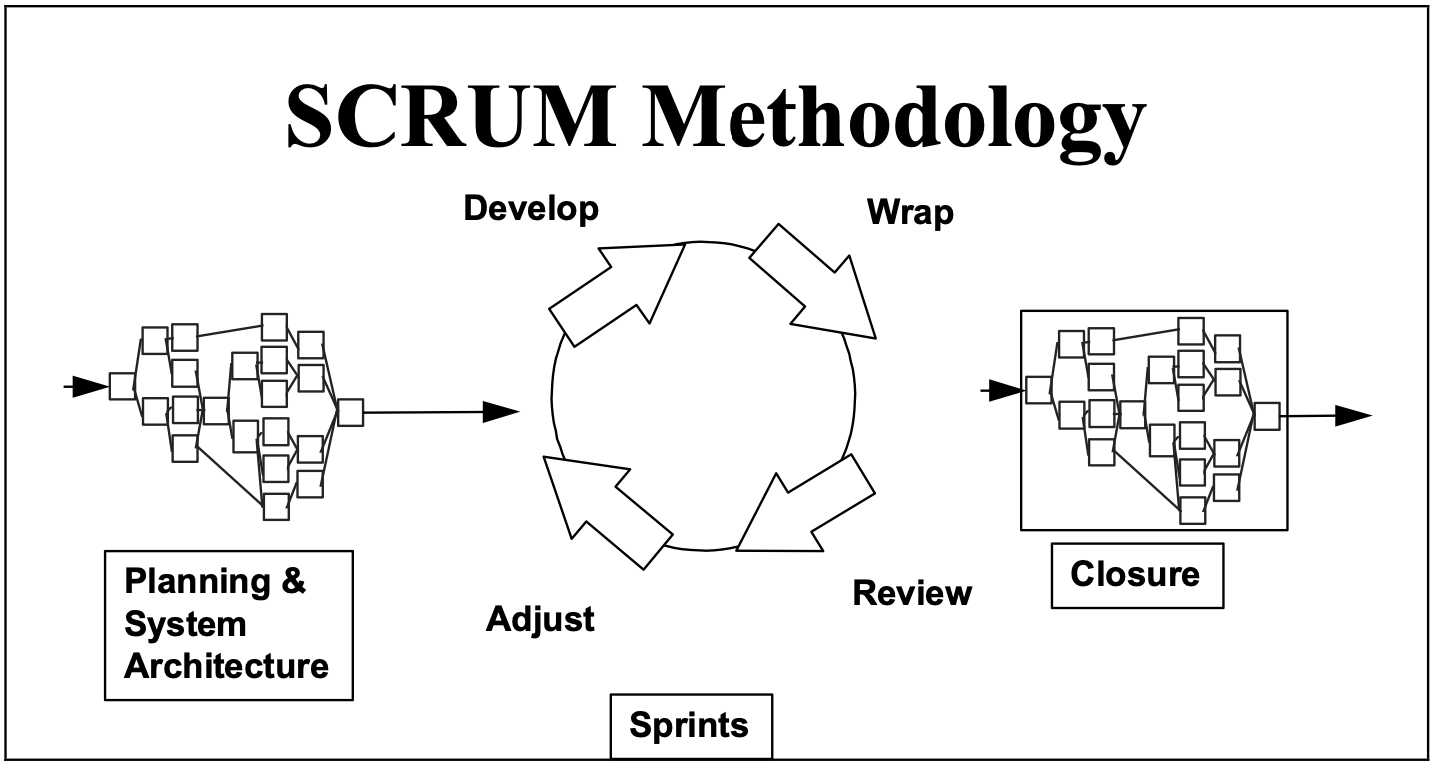
\includegraphics[scale=0.45]{imagenes/scrum.png}}  
        \caption{Fases de la metodología SCRUM \cite{schwaber1997scrum}} \label{fig:figura1}
    \end{figure}

\begin{itemize}
    \item \textbf{Pregame:} 
    \begin{itemize}
        \item \textit{Planificación:} En esta fase se crea la lista de tareas a realizar (backlog list), se fija la fecha de entrega del producto y su funcionalidad, se forma el equipo (o equipos) de trabajo, se valoran los riesgos que puedan surgir, los costes y finalmente se revisa todo y se aprueba el proyecto.
        \item \textit{Arquitectura/Diseño de alto nivel:} Se revisan los elementos en el backlog, se realizan cambios si es necesario para poder implementarlos, se perfila la arquitectura del sistema teniendo en cuenta estos cambios y una reunión es organizada para revisar el diseño, donde cada equipo presenta una propuesta para implementar cada backlog.
    \end{itemize}
    \item \textbf{Game:} Corresponde con el conocido Sprint de la metodología SCRUM. Es la parte iterativa de la metodología, que se ejecuta varias veces hasta conseguir el producto final y está formada por las siguientes subtareas:
    \begin{itemize}
        \item \textit{Desarrollo:} Lo primero que se realiza es definir los cambios que hay que realizar en los backlogs para poder implementarlos. Se dividen las tareas presentes en el backlog en paquetes, y se completan estos paquetes diseñando, desarrollando, implementando, testeando y documentando los cambios.
        \item \textit{Envoltura:} Se cierran los paquetes, creando una ejecutable que incorpora los cambios y se explica como cumplen lo especificado en los backlogs.
        \item \textit{Revisión:} Todos los equipos se reunen para presentar el trabajo. El desarrollo obtenido se evalúa y se añaden nuevas tareas que puedan surgir al backlog. Se evalúa el riesgo y se realizan propuestas en base a este.
        \item \textit{Ajuste:} Se consolida la información recibida durante la revisión.
    \end{itemize}
    
    \item \textbf{Postgame:}
    \begin{itemize}
        \item \textit{Cierre:} Cuando el gestor del proyecto considera que el producto está terminado y cumple con los requisitos solicitados por el cliente se entra en esta fase, donde se prepara el producto para su despliegue. Integración, generación de la documentación, testeo y marketing son algunas de las actividades que se realizan en este paso.
    \end{itemize}

\end{itemize}

Estas características que hemos mencionado son las especificadas en la definición original de SCRUM. Aún así, en la práctica cada proyecto las adapta a sus necesidades. En general, los sprints suelen tener una duración de 2 o 3 semanas. En nuestro caso tendrán 1 o 2 semanas de duración.



\chapter{Estado del arte}
Para poder organizar este proyecto debemos conocer el estado del arte en su ámbito. Hablaré sobre el estado de arte en cheminformatics, en Deep Learning y sobre las herramientas que se han creado en estas áreas del conocimiento y que  van a facilitar el desarrollo de este TFG.

\section{Cheminformatics}
Como comenté en el Capítulo \ref{intro}, cheminformatics es un tema muy amplio y engloba subtópicos diferentes. Muchos de ellos surgieron en la década de 1960 y principios de 1970, y desde esa época muchos grupos de investigación siguen trabajando en ellos y nuevos grupos han surgido para aplicar nuevas tecnologías en nuevos ámbitos. A continuación, se discuten algunos de los temas que históricamente han sido de interés para esta ciencia. \cite{doi:10.1021/ci600234z}

\subsection{Compuestos orgánicos y su representación}
Un compuesto orgánico es un compuesto químico que contiene átomos de carbono \cite{mcmurry2008quimica}. En el conjunto de datos sobre el que trabajo, los ejemplos positivos son concretamente compuestos químicos organometálicos, en los que átomos de carbono forman enlaces covalentes con átomos metálicos \cite{mcmurry2008quimica}.

En las publicaciones de química encontramos numerosas representaciones gráficas de estos compuestos, lo que se conocen como fórmulas estructurales. Estas muestran la disposición en el espacio de los átomos que forman el compuesto. Un ejemplo es la siguiente figura:

\begin{figure}[H]
\centering
    \fbox{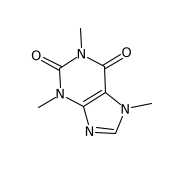
\includegraphics[scale=0.7]{imagenes/caffeine.png}}  
    \caption{Estructura de la cafeína. \cite{decimer}}
    \label{fig:caffeine}
\end{figure}

\noindent En ellas pueden aparecer multitud de elementos, apareciendo siempre:
\begin{itemize}
    \item \textbf{Átomos:} Se sitúan en los extremos de los enlaces. Representados con letras que indican el elemento químico del que se trata, tal y como aparece en la tabla periódica.
    \item \textbf{Enlaces:} Unen dos átomos entre sí. 
\end{itemize}

En algunas ocasiones, sobre los átomos pueden mostrarse cargas positivas o negativas representando iones. Aparte, puede mostrarse lo que se conoce como información estereoquímica, que indica la disposición de los átomos en el espacio. Ésta es importante ya que afecta a las propiedades y reactividad de las moléculas \cite{wade2004quimica,structrep}.

\begin{figure}[H]
\centering
    \fbox{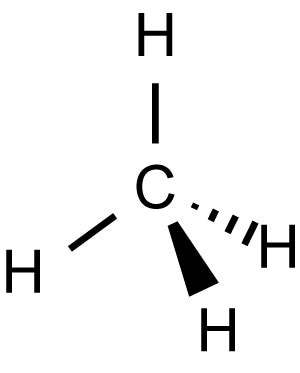
\includegraphics[scale=0.5]{imagenes/methane.jpg}}  
    \caption{Estructura del metano. \cite{structrep}} 
    \label{fig:metano}
\end{figure}

En la Figura \ref{fig:metano}:
\begin{itemize}
    \item Las líneas sólidas representan enlaces en el plano.
    \item Las discontinuas representan enlaces que están más alejados.
    \item Aquellas con forma de cuña indican que uno de los átomos se encuentra más cerca del espectador. 
\end{itemize}

Además, un mismo compuesto se puede representar de distintas formas:
\begin{figure}[H]
\centering
    \fbox{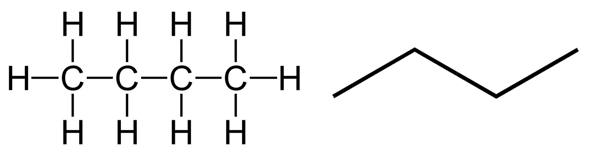
\includegraphics[scale=0.3]{imagenes/skeletal.png}}
    \caption{Dos formas de representar el butano. \cite{structrep}}
    \label{fig:butano}
\end{figure}

En la Figura \ref{fig:butano}, en a) se detalla la definición de todos los átomos, en cambio en b) encontramos lo que se conoce como fórmula de esqueleto, donde se omiten los átomos de carbono e hidrógeno. Se sabe que hay un átomo de carbono en los vértices que quedan libres en la intersección de dos enlaces o en las terminaciones donde no aparece ningún otro elemento. Se supone a la vez que cada átomo de carbono tiene cuatro enlaces, por tanto el número de enlaces que faltan por indicar explícitamente se corresponden con enlaces a moléculas de hidrógeno \cite{wade2004quimica,structrep}.


\subsection{Representación en el ordenador}
El poder almacenar representaciones de compuestos químicos de manera eficiente en un ordenador requiere de la creación de métodos y formatos específicos para ello. Además, hay que tener en cuenta qué datos vamos a codificar, si solo la estructura básica del compuesto, si también se quiere guardar información estereoquímica o si queremos añadir notas auxiliares sobre los compuestos. Es importante tener esto claro, ya que la complejidad de la representación influirá en la cantidad de almacenamiento que ocupe en disco y en los recursos necesarios para procesarla.

Utilizando notación lineal, se representa la estructura del compuesto como una secuencia lineal de caracteres y números. Esta es una codificación adecuada para las computadoras, ya que la pueden procesar con facilidad. Algunos formatos que utilizan esta notación son WLN (Wiswesser Line Notation), ROSDAL (Rp) o SMILES (Simplified Molecular Input Line Entry Specification). Aunque WLN y ROSDAL han quedado obsoletos, SMILES se sigue utilizando con mucha frecuencia en la actualidad. \cite{doi:10.1021/ci600234z}

\begin{figure}[H]
\centering
    \fbox{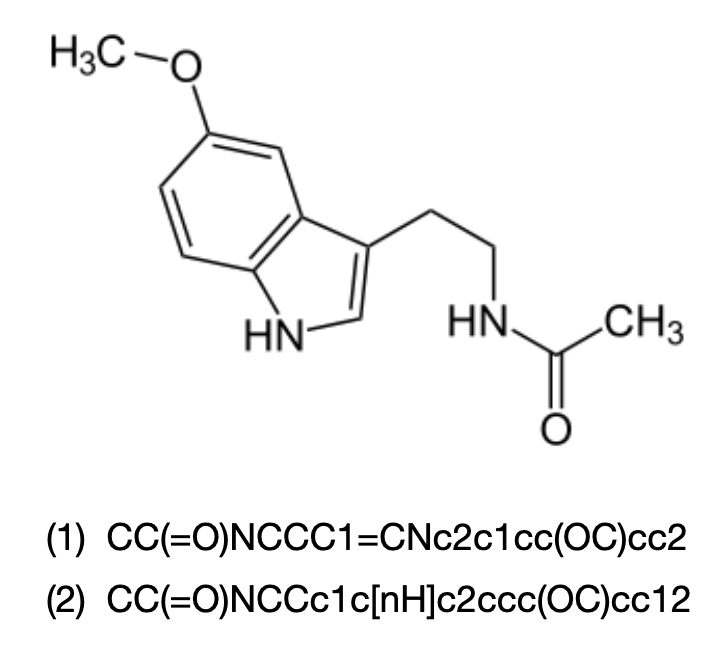
\includegraphics[scale=0.25]{imagenes/smiles_melatonina.png}}  
    \caption{Dos posibles codificaciones de la melatonina en SMILES. \cite{smiles_wikimedia}}
    \label{fig:ciclos-smiles}
\end{figure}

Aunque no voy a entrar en detalle de cómo funciona ya que para ello hay que tener nociones avanzadas de química, diremos que utiliza las siglas de cada elemento de la tabla periódica para representar los átomos. La primera letra del elemento se escribe en mayúscula, a no ser que se trate de un átomo perteneciente a un anillo aromático\footnote{La aromaticidad es una propiedad presente en moléculas cíclicas que contienen anillos de seis elementos similares a los del benzeno con tres enlaces dobles. Esto mejora la estabilidad del compuesto. \cite{aromaticidad, mcmurry2008quimica}}, ya que en ese caso se escribe en minúscula. Si el elemento tiene dos caracteres, el segundo se escribe siempre en minúscula. Además, se pueden representar cargas.

Los enlaces se representan con -, =, \# y :, según el tipo. Bajo algunas circunstancias, se pueden omitir estos símbolos, ya que por su contexto se deducen. También se pueden codificar ramas, situando elementos entre paréntesis, y ciclos, utilizando un número para indicar el inicio y el fin del ciclo en la cadena de texto, como se observa en la Figura \ref{fig:ciclos-smiles}. \cite{weininger1988smiles}

\begin{figure}[H]
\centering
    \fbox{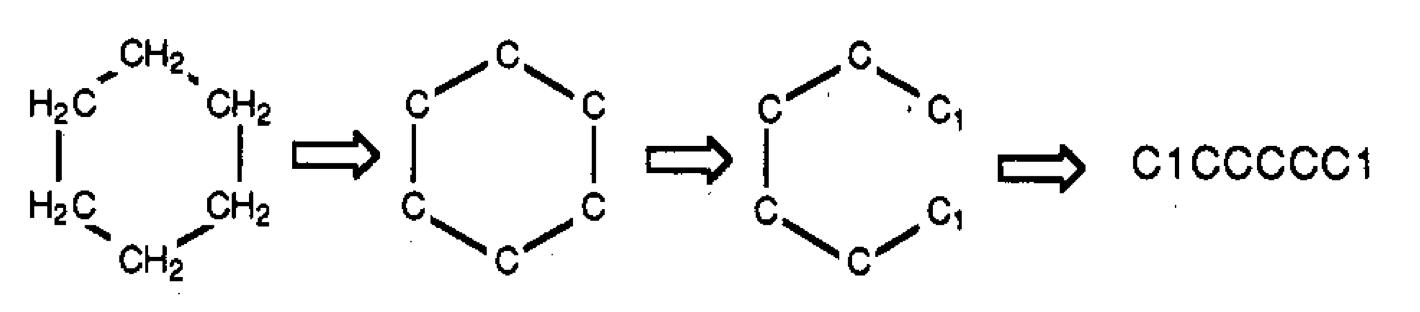
\includegraphics[scale=0.35]{imagenes/smiles_cycle.png}}  
    \caption{Ciclos en SMILES. \cite{weininger1988smiles}}
    \label{fig:ciclos-smiles}
\end{figure}

Otras características como la aromaticidad o estructuras inconectas también pueden ser representadas. Entre las ventajas de esta codificación, destaca su facilidad de comprensión por los humanos. Cualquier químico puede aprender sus reglas de codificación fácilmente y diseñar sus propios compuestos. Un problema que tiene SMILES es que un mismo elemento se puede representar de diferentes formas (Figura \ref{fig:ciclos-smiles}). Pero sobre todo, el mayor problema es que un porcentaje significativo de las cadenas no se corresponden con moléculas válidas, ya sea porque son sintácticamente inválidas, no se corresponden con un grafo molecular o no cumplen reglas químicas básicas. \cite{weininger1988smiles}

Uno de los principales objetivos de la química computacional es el diseño de nuevas moléculas. Para ello, la utilización de modelos generativos puede ayudar a los investigadores, pero si el espacio de estados de SMILES no es completamente válido se dificulta la tarea. Para ello han surgido otras codificaciones como SELFIES con un espacio 100\% robusto. \cite{Krenn_2020}

Además de estos formatos de notación lineal, es necesario mencionar otros. El lanzamiento en 1982 de MDL MOLfile llevó a su aceptación como principal formato para codificar compuestos químicos. La estructura que siguen estos archivos se muestra en la figura \ref{fig:molfile}. Se han realizado distintas adaptaciones de este para añadir información extra a las moléculas, dando lugar a SDfile (puede agrupar más de un MOLfile y almacenar información estructural), RXNfile (anota los reactivos y productos de una única reacción química), etc \cite{doi:10.1021/ci00007a012}. El formato PDB se utiliza principalmente para almacenar información 3D de macromoléculas biológicas, como son las proteínas o los polinucleótidos. CIF también es un formato para almacenar información 3D. En espectroscopia se encuentra JCAMP. Finalmente, CML (chemical markup language), una extensión de XML, es una propuesta que intenta aglutinar toda la información disponible. Es compatible con moléculas, reacciones, espectroscopia y otra información. \cite{doi:10.1021/ci600234z}

\begin{figure}[H]
\centering
    \fbox{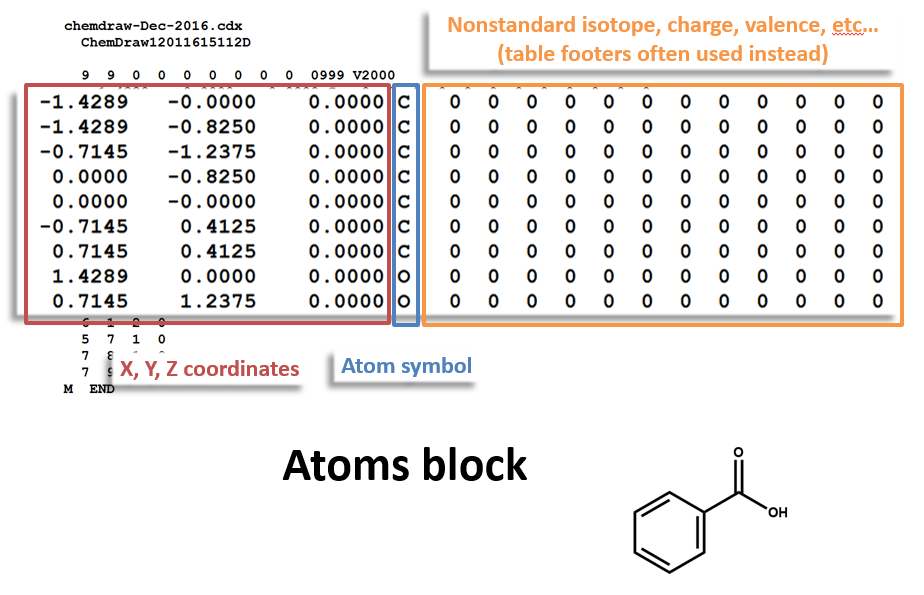
\includegraphics[scale=0.32]{imagenes/molfile.png}}  
    \caption{Contenido de un archivo MOL. \cite{molfile_example}} 
    \label{fig:molfile}
\end{figure}


\subsection{Fuentes y bases de datos}

El gran número de facetas que presenta la información química necesita sistemas de almacenamiento a la altura. La química fue una de las primeras ramas científicas en utilizar bases de datos para almacenar: la cantidad de datos que se generaba creció rápidamente, y sigue creciendo hoy en día. 

Aunque es complicado clasificarlas, vamos a separarlas en tres grandes grupos según el tipo de información que almacenan: \cite{doi:10.1021/ci600234z}
\begin{itemize}
    \item \textbf{Bases de datos de publicaciones:} Pueden ser bibliográficas, guardando solamente los metadatos y la referencia a la publicación, o de texto completo, donde recogen la publicación de forma íntegra. %TODO: Qué son las publicaciones primarias?
    \item \textbf{Bases de datos fácticas:} Al contrario que las anteriores, que almacenan publicaciones de la literatura primaria, estas pueden guardar propiedades físicas de compuestos, información de espectroscopia, información legal, etc.
    \item \textbf{Bases de datos de estructuras y reacciones:} Recogen estructuras químicas, tanto individualmente como formando parte de reacciones. No se almacenan como imágenes, sino en formatos interpretables por la máquina.
    \item \textbf{Bases de datos de biología molecular:} Contienen secuencias de aminoácidos y nucleótidos.
\end{itemize}

Pero, ¿cómo se pueden rellenar con datos? ¿De dónde se pueden extraer? Durante décadas se han publicado un gran número de artículos. Se podrían utilizar como una fuente muy amplia de información, ya que contienen todo el progreso científico. Específicamente para extraer datos relativos a estructuras entran en juego utilidades conocidas como OCSR (Optical Chemical Structure Recognition).

Son capaces de transformar una imagen en un formato compatible con la máquina, como podría ser SMILES. En muchos casos incluso es posible introducirles una publicación completa y ellas mismas localizan las imágenes de moléculas. Con el paso del tiempo se han ido perfeccionando, y algunas son capaces de detectar información estereoquímica o de relacionar el compuesto con el texto de la publicación. ChemEx \cite{tharatipyakul2012chemex}, ChemGrapher \cite{oldenhof2020chemgrapher} y DECIMER \cite{rajan2020decimer} son ejemplos de sistemas OCSR publicados en la última década.

Por último, mencionar una base de datos que merece la pena conocer. Creada por el National Institute of Health (NIH), PubChem es una base de datos abierta que cada mes sirve a millones de usuarios en todo el mundo. Es una base de datos de estructuras y aunque contiene mayoritariamente moléculas pequeñas, también almacena nucleótidos, carbohidratos, lípidos, péptidos y macromoléculas modificadas químicamente. Para cada compuesto almacena su estructura, identificadores, propiedades físicas y químicas, toxicidad, patentes, etc. Los datos que aglutina provienen de diversas fuentes, como son agencias del gobierno estadounidense, editores de revistas científicas o proveedores químicos, aunque hay muchas más. \cite{pubchem}

\subsection{Métodos de búsqueda}
Almacenar información en las bases de datos no sirve de nada si no se desarrollan métodos eficientes para extraerla. En aquellas bases de datos donde se almacenan estructuras químicas, una de las principales formas de obtener información es buscar similitudes entre una molécula dada como entrada y otras que se encuentran almacenadas, de forma que compartan una subestructura específica o tengan otras características en común. Para ello, es clave la codificación de los compuestos.

También, si se almacenan metadatos y la base de datos está indexada sobre ellos se podría buscar por su nombre, etiquetas, etc. \cite{doi:10.1021/ci600234z}

\subsection{Métodos para análisis de datos}
En química, grandes cantidades de datos son producidas. Una vez que hemos conseguido limpiarlos y ordenarlos, tenemos un conocimiento muy valioso en nuestras manos. La información es muy interesante en sí misma, pero también lo son las relaciones que se esconden en su interior. Para ello, se crean modelos que puedan interiorizarlas.

El análisis de datos no solo se enfrenta a la extracción de la información principal, sino que también intenta generar nueva información secundaria. \cite{doi:10.1021/ci600234z}

Este TFG se desarrolla dentro de este ámbito ya que, como describiré más adelante, entreno un modelo capaz de detectar que imágenes contienen moléculas.

\newpage
\section{Deep learning}
En las últimas décadas, la Inteligencia Artificial (I.A.) ha vivido un periodo de crecimiento brutal. Dentro del ámbito de la I.A. se engloban técnicas muy diferentes que tienen como objetivo simular el comportamiento inteligente de los seres vivos, siendo uno de sus rasgos la capacidad de aprendizaje. Los sistemas expertos fueron su primer éxito comercial. En ellos se codificaban una serie de reglas manualmente, emulando el razonamiento de un experto en un problema específico.

El aprendizaje automático es un subconjunto dentro de la Inteligencia Artificial. Aglutina aquellas técnicas que permiten a un ordenador construir modelos a partir de conjuntos de datos, aprendiendo con la experiencia. No hace falta definir reglas de forma explícita. Pero tiene un inconveniente, y es que en muchos casos un especialista humano tiene que elegir manualmente que características de los datos son relevantes en el problema.

El aprendizaje profundo o deep learning va un paso más allá. Es un subconjunto del aprendizaje automático, pero en las técnicas que engloba no es necesario indicar al modelo las características útiles, ya que él mismo las descubre automáticamente. Y no se queda ahí, puede incluso generar nuevas características a partir de las existentes.

El desarrollo temporal de estas técnicas coincide con el orden en el que las menciono. Como se puede apreciar, el proceso de aprendizaje consta de diferentes fases, de las que cada vez se encuentra automatizado un mayor número. \cite{berzal2018redes}

Casi todos los algoritmos de deep learning son una adaptación particular de un proceso que se puede resumir en los siguientes cuatro pasos:

\begin{itemize}
    \item Extraer un conjunto de datos asociado al problema (un conjunto de gran tamaño, cuanto más grande mejor).
    \item Diseñar una función de coste apropiada (loss function).
    \item Crear un modelo y definir sus hiperparámetros (tamaño, tasa de aprendizaje...), asignándole los valores más adecuados.
    \item Aplicar un algoritmo de optimización para minimizar la función de coste.
\end{itemize}

Siendo esta la estrategia que se utiliza en otras muchas técnicas de aprendizaje automático. La diferencia entre el deep learning y estas otras es la capacidad de abstracción que tiene el primero, que viene dada por la capacidad de jerarquizar la información en distintas capas utilizando múltiples niveles de representación. Esta abstracción permite separar la esencia de lo prescindible, de forma que los modelos pueden aprender qué relaciones entre los datos son importantes y cuáles son simples accidentes, y consecuentemente generalizar de forma adecuada. \cite{berzal2018redes}

\subsection{Redes neuronales multicapa}
Nuestro cerebro contiene un tipo especial de células llamadas neuronas. Estas reciben impulsos eléctricos que son capaces de atenuar o amplificar para posteriormente enviarlos a otras neuronas. La unión de millones de estas crea una estructura neuronal que es la que nos permite pensar y actuar como seres inteligentes.

En la informática se ha intentado emular este comportamiento, creando lo que se conoce como redes neuronales artificiales. Las neuronas artificiales omiten muchas características que definen a las biológicas, como su localización espacial, los retardos en la propagación de señales o los mecanismos químicos de sodio y potasio que permiten la transmisión de potenciales eléctricos. Al final, un modelo es una representación de la realidad, y por tanto contiene información más limitada que esta. El modelo de integración y disparo define la base de la neurona que se utiliza habitualmente en Inteligencia Artificial, representado en la Figura \ref{fig:integracion-disparo}.

\begin{figure}[H]
\centering
    \fbox{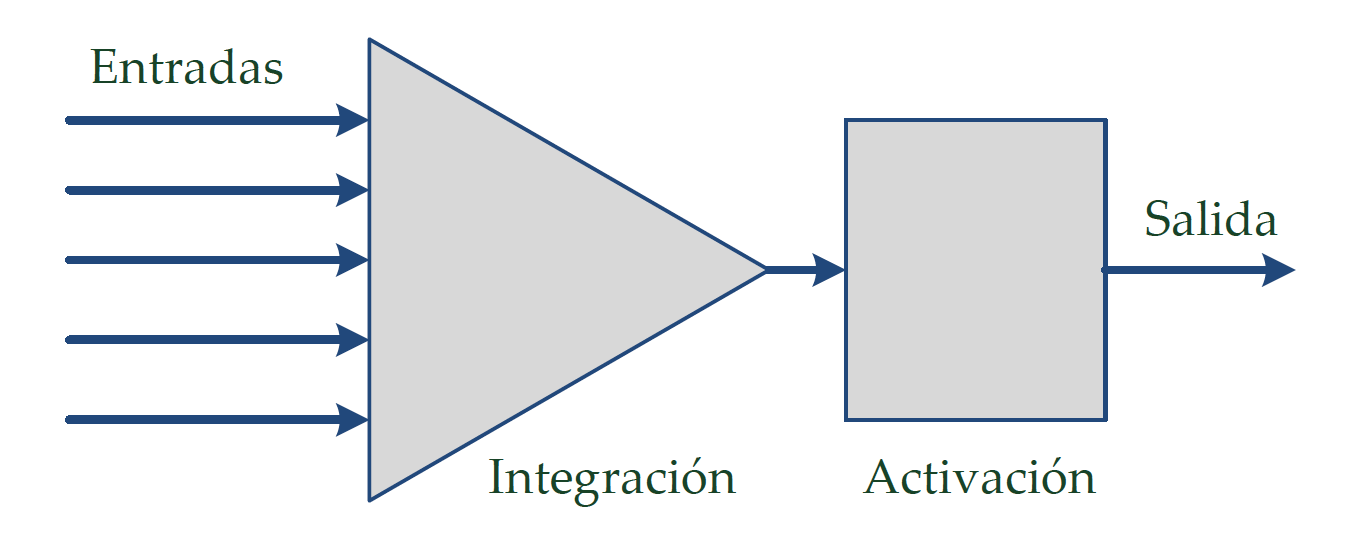
\includegraphics[scale=0.4]{imagenes/integracion_disparo.png}}  
    \caption{Modelo de integración y disparo en las neuronas artificiales \cite{berzal2018redes}}
    \label{fig:integracion-disparo}
\end{figure}

En la fase de integración se unifican todas las señales $x_i$ entrantes a la neurona $j$, cada una influyendo en mayor o menor medida según el peso $w_{ij}$, peso de la conexión de la neurona $i$ hasta la neurona $j$:

\begin{equation}
    z_j = b_j + \sum_{i=1}^{n} x_iw_{ij}
\end{equation}

Además, en muchas ocasiones se añade la componente $b_j$ que actúa como sesgo, permitiendo que la salida de la neurona se desplace a la izquierda o a la derecha en el eje X. Este sesgo también se puede representar de forma implícita, de forma que $i$ parte de 0 en vez de 1, siendo $x_0 = 1$ y $w_0j = b_j$. \cite{berzal2018redes}

Pero esta fase de integración no es suficiente para simular el comportamiento del cerebro humano, su resultado es lineal. Una red neuronal se genera encadenando capas de estas neuronas, donde la salida de las neuronas de una capa actúan de entrada a las neuronas de la siguiente capa. La combinación de funciones lineales es una función lineal, y por tanto el resultado final de la red seguiría siendo una función lineal de las entradas. En definitiva, tener $n$ capas equivaldría a utilizar una única capa.

Es por ello que existe una segunda fase en este proceso, la fase de activación. Al resultado de integración en cada neurona se le aplica una función de activación no lineal ($\sigma$). A partir de ahora, nuestra red podrá aproximar funciones no lineales: cuantas más capas se utilicen en una red, con mayor precisión se podrá llevar a cabo esta aproximación.

\begin{equation}
    f_j = \sigma(z_j) = \sigma(b_j + \sum_{i=1}^{n} x_iw_{ij})
\end{equation}

\noindent $f_j$ es la salida final de la neurona. \cite{berzal2018redes}

\subsection{Redes neuronales convolutivas}
Si hay una técnica del aprendizaje profundo que funcione especialmente bien en la práctica, son las redes neuronales convolutivas o convolutional neural networks (CNN). Estas se utilizan para procesar señales, como son las imágenes.

Una ventaja frente a las redes multicapa reside en que pueden trabajar con entradas y salidas estructuradas. Esto supone que, en vez de recibir un vector de entradas correspondientes a diferentes variables, pueden trabajar directamente con un vector 1D, una matriz 2D o con un tensor con múltiples dimensiones. \cite{berzal2018redes} 

En estas redes, las capas realizan la operación de convolución en vez de la multiplicación de las entradas por pesos. En el caso de imágenes (señal 2D), esta operación se define como:

\begin{equation}
    S(i,j) = (I*K)(i,j) = \sum_m \sum_n I(m,n)K(i-m,j-n)
\end{equation}

Donde $I$ representa una imagen y $K$ un kernel de dos dimensiones \cite{Goodfellow-et-al-2016}. El tipo de convolución que describimos aquí es la discreta y por ello en la fórmula aparecen sumatorias, en vez de las integrales típicas de dominios continuos. En la Figura \ref{fig:ejemplo-convolucion} se puede observar un ejemplo de convolución.

\begin{figure}[H]
\centering
    \fbox{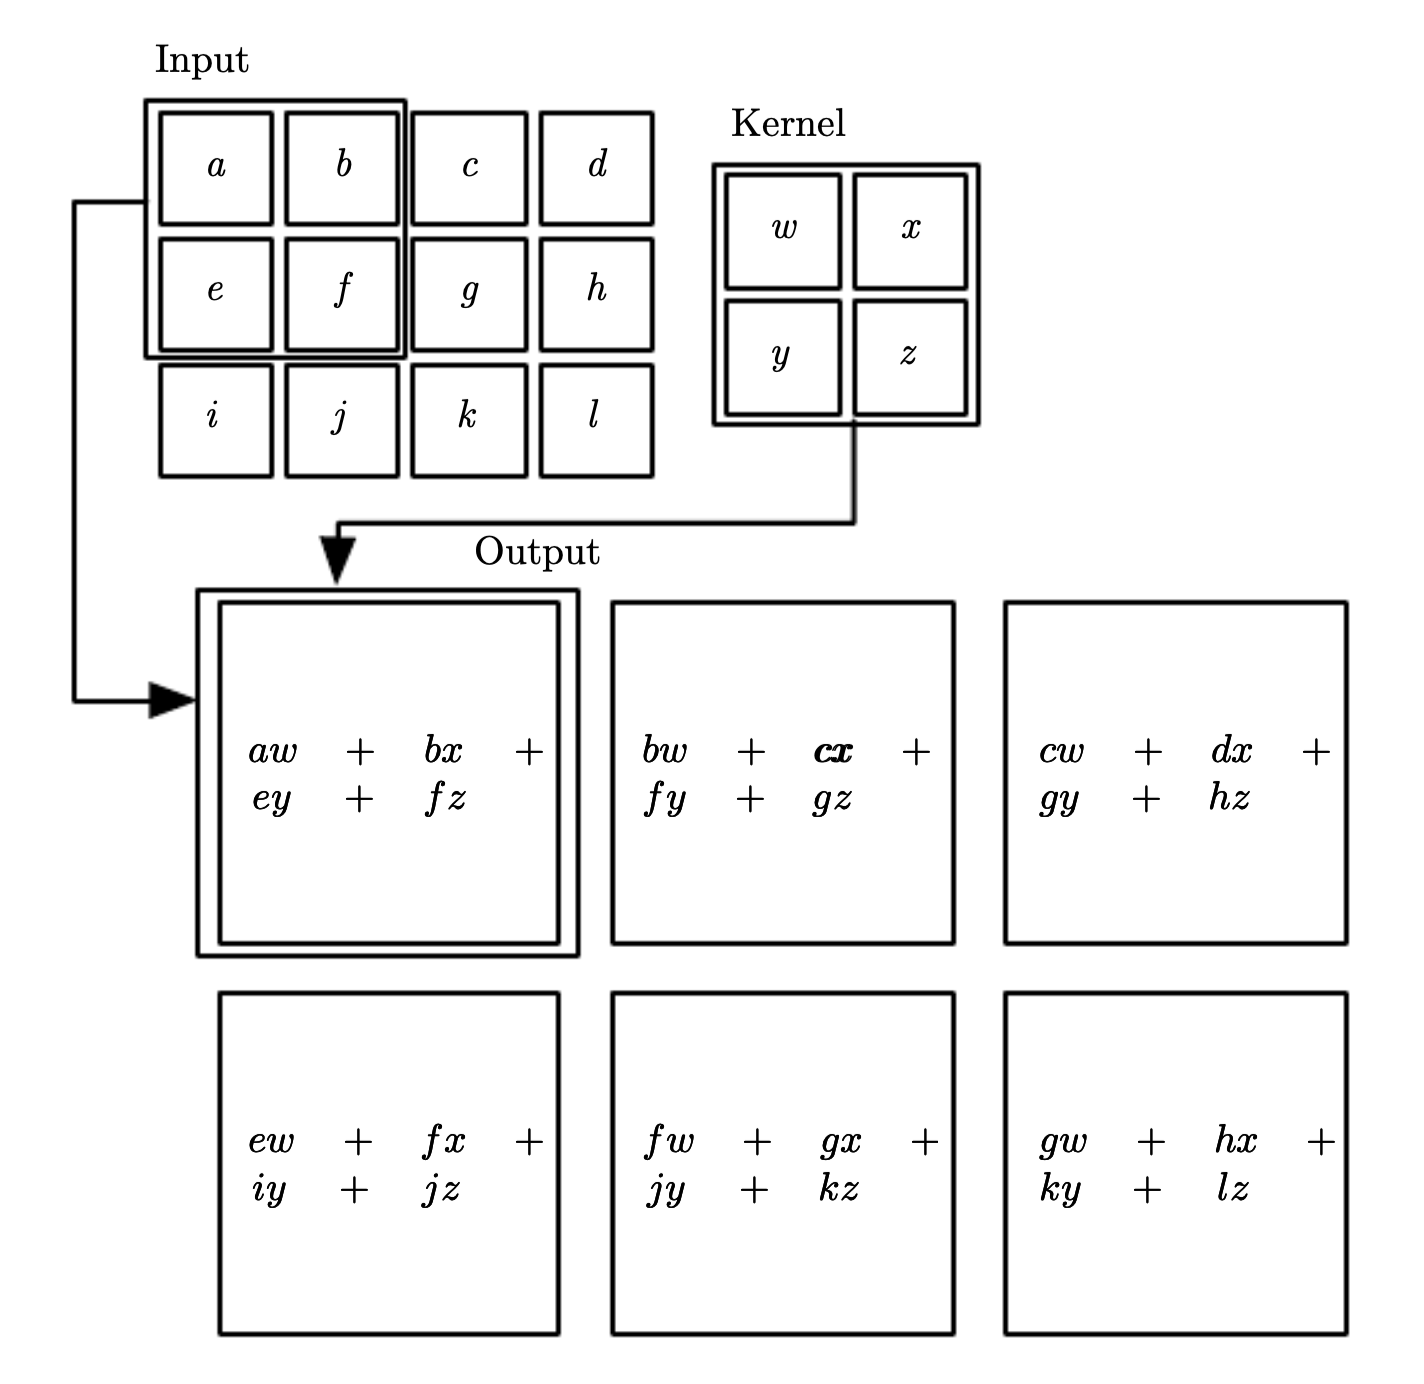
\includegraphics[scale=0.4]{imagenes/convolution.png}}  
    \caption{Resultado de convolucionar la entrada I con el kernel K \cite{Goodfellow-et-al-2016}}
    \label{fig:ejemplo-convolucion}
\end{figure}

El kernel se va desplazando por la imagen, solapándose sobre cierta área de esta. En cada una de las posiciones que toma genera un valor de salida, fruto de la multiplicación del valor de los píxeles de la imagen sobre los que se encuentra por los pesos del kernel. Todos estos valores de salida forman el resultado final, que mantiene la misma estructura 2D (aunque normalmente con un menor tamaño). 

Así es como funcionan las redes neuronales convolutivas, donde cada capa de la red aplica este operador a la entrada que recibe. Con ellas:
\begin{itemize}
    \item Se reduce el número de parámetros necesarios. Este depende del tamaño de los kernel utilizados, que suele ser muy inferior al de las imágenes de entrada.
    \item Se mantienen las relaciones espaciales/temporales de las señales. Muy beneficioso en análisis de imágenes, donde dos pixeles cercanos contendrán información similar. Los capas convolutivas son capaces de interpretar estas relaciones y mantenerlas para las siguientes fases del modelo. \cite{Goodfellow-et-al-2016}
\end{itemize}

\subsection{Autocodificadores}
Los autocodificadores o autoencoders son un modelo de aprendizaje no supervisado que permite encontrar una representación latente no lineal para una distribución de datos dada.

Para comprenderlos correctamente, definamos primero lo que es una representación latente. Esta es una representación subyacente para una determinada distribución de datos, es decir, una forma ``comprimida" de representar la distribución que siguen estos. En esta representación, se reduce el número de dimensiones necesarias para definir la distribución.

Existe un algoritmo conocido como análisis de componentes principales (\textit{Principal Component Analysis}, PCA) que encuentra una transformación de la representación original a otra latente. Pero tiene un problema, y es que como su transformación es lineal. \cite{vqvae}

Los autocodificadores realizan esta tarea pero encontrando una transformación no lineal, por lo que pueden trabajar con datos más complejos. Para ello constan de dos partes, el codificador y el decodificador (Figura \ref{fig:autocodificador}).

\begin{figure}[H]
\centering
    \fbox{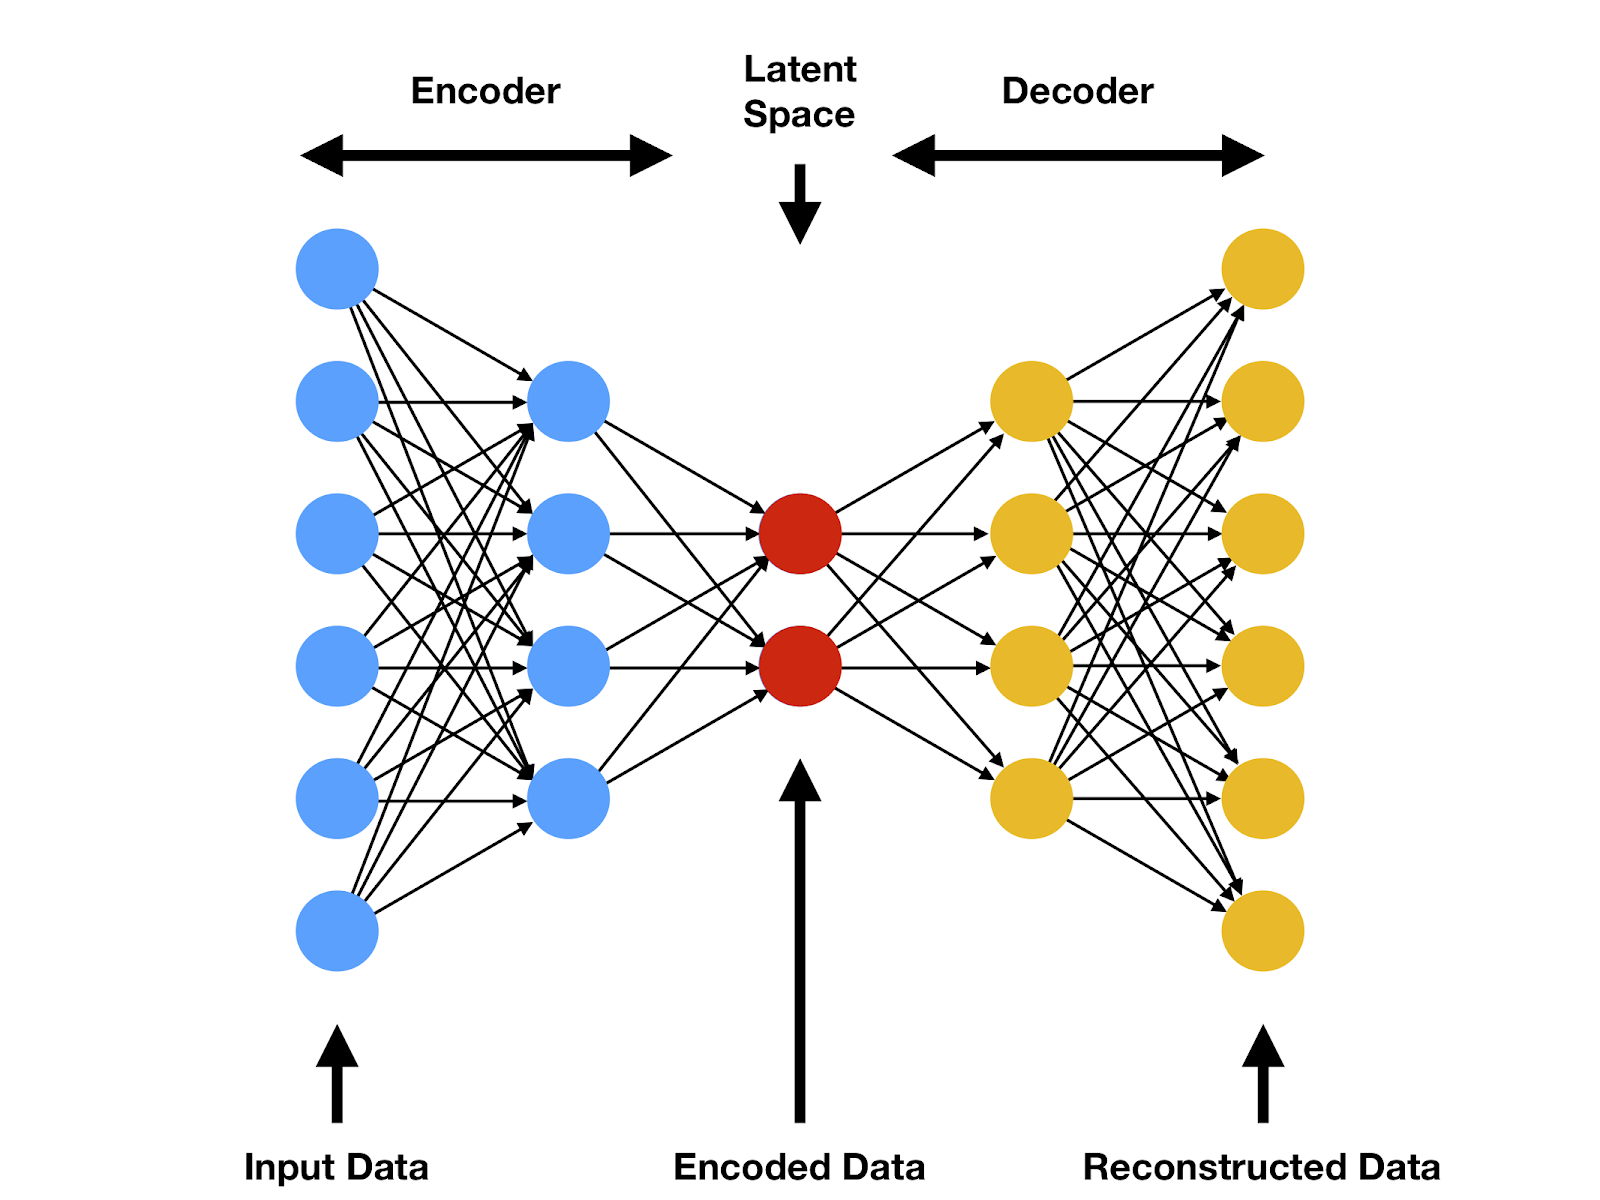
\includegraphics[scale=0.18]{imagenes/autoencoder.png}}
    \caption{Secciones en las que se divide un autocodificador \cite{vqvae}}
    \label{fig:autocodificador}
\end{figure}

El objetivo tras el entrenamiento del modelo es que los datos reconstruidos por el decodificador sean lo más parecidos posible a los de entrada.

Un tipo especial de autocodificador es el autocodificador variacional (Variational Autoencoder, VAE). La principal diferencia viene dada por la estructura que sigue la representación latente, donde se fuerza al autocodificador a organizarla de forma que puntos de datos similares se encuentren cerca y puntos diferentes se encuentren separados, como se aprecia en la figura \ref{fig:vae}. En un autocodificador regular esto no se exige, por lo que no podríamos desplazarnos por el espacio latente y observar cambios graduales que se corresponden con cambios graduales en la representación original. \cite{vqvae}

\begin{figure}[H]
\centering
    \fbox{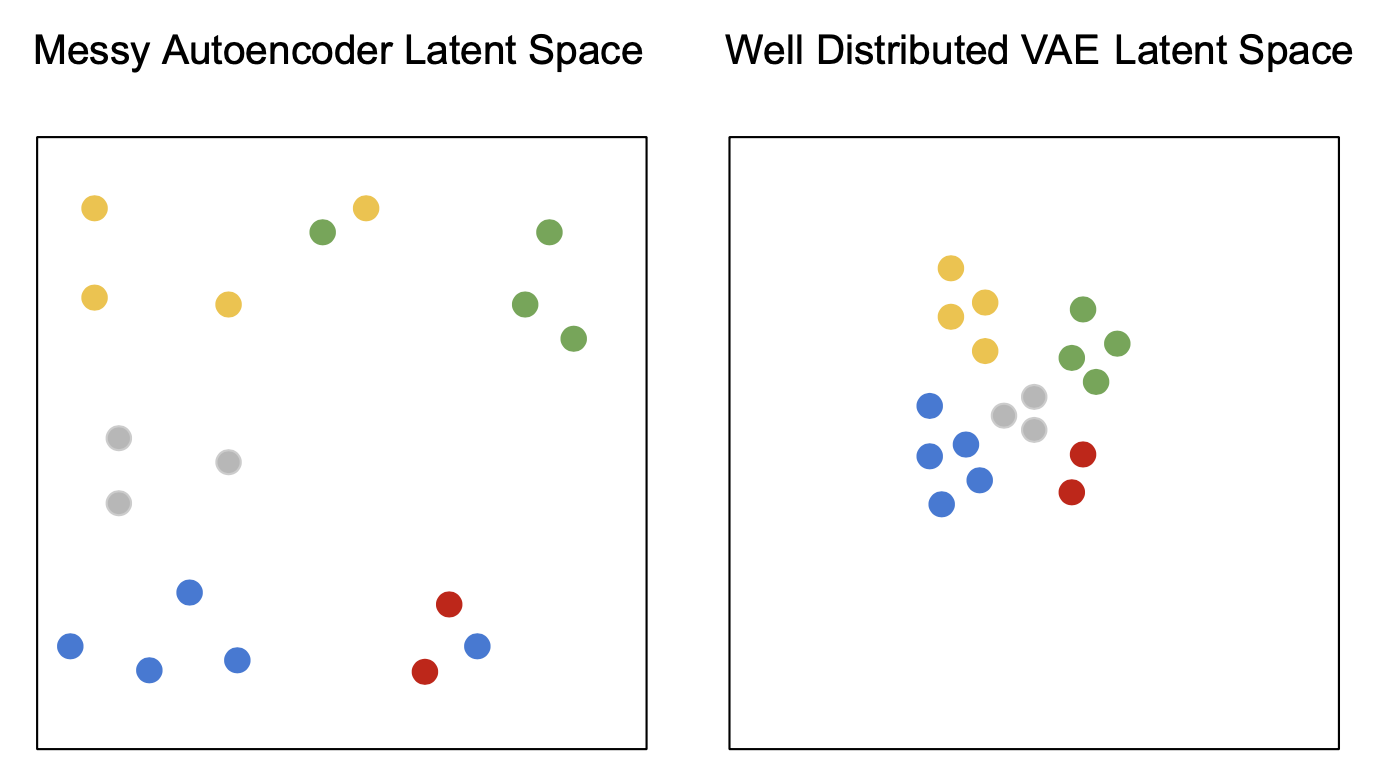
\includegraphics[scale=0.23]{imagenes/vae.png}}  
    \caption{Espacio latente en un autocodificador regular vs en VAE \cite{vqvae}}
    \label{fig:vae}
\end{figure}

\subsubsection{Vector Quantized Variational Autoencoder}
La representación latente por defecto en los VAE es continua. Pero existe una variante en la que se discretiza esta representación. Esto es útil cuando trabajamos con datos como imágenes: podría utilizarse una variable discreta para el color, otra para el tipo de objeto, su tamaño, etc. Muchos otros elementos del mundo real son susceptibles de representarse de forma discreta. Hay modelos como los transformers, que voy a presentar más adelante, que están diseñados para trabajar sobre datos con esta codificación. \cite{vqvae}

Los Vector Quantized Variational Autoencoders (VQVAE) utilizan este tipo de codificación, donde la representación latente consiste en lo que se conoce como libro de código (codebook). Este codebook no deja de ser un conjunto de vectores discretos asociados a un índice.

Cuando el codificador recibe un dato, este se transforma a la representación latente. A continuación, se introduce al decodificador el vector del codebook con el que existe una menor distancia euclídea. Este vector es procesado por el decodificador devolviendo la salida final. Dicho esto, se podría pensar que la potencia expresiva del autoencoder es muy baja, ya que el número de vectores del codebook es mucho más pequeño que el conjunto de posibles datos de entrada, y siempre que se introdujese el mismo vector al decodificador obtendríamos la misma salida.

Esto no es así, ya que normalmente no se utiliza un único vector: en datos como imágenes, es probable que se escoja un conjunto de vectores que se introducen en el decodificador. Estos son procesados conjuntamente y finalmente se devuelve la imagen sintética. De esta forma, el número de posibilidades crece enormemente. \cite{vqvae}

\subsection{Redes generativas antagónicas}
En inglés conocidas como Generative Adversarial Networks (GANs), son un tipo de modelos utilizados para generar datos sintéticos, que por ejemplo pueden servir para ampliar nuestro dataset. Contienen dos módulos que trabajan simultáneamente, cada uno de ellos intentando ser mejor que el otro. Estos dos módulos son el generador G y el discriminador D: el generador intenta crear datos sintéticos parecidos a los reales y el discriminador actuará de juez, tendrá que decidir si dado un dato este es real o sintético.
Estamos en un juego en el que el generador intentará mejorar todo lo posible para generar imágenes indistinguibles a ojos del discriminador, desarrollándose en dos escenarios: \cite{berzal2018redes}

\begin{itemize}
    \item Se muestrean datos x del conjunto de entrenamiento y se introducen en D. En este caso, D(x) será un valor cercano a 1, ya que las muestras son datos reales.
    \item Se introduce en G una muestra z generada aleatoriamente de acuerdo a una distribución de probabilidad, siendo G(z) una muestra sintética. D(G(z)) deberá tomar un valor cercano a 0, detectando que no se trata de una muestra real. Sin embargo, aunque el discriminador actúa para que D(G(z)) sea cercano a 0, el generador hace todo lo contrario y pretende que D(G(z)) se aproxime a 1.
\end{itemize}

El entrenamiento se lleva a cabo simultáneamente en G y D, actualizando los pesos de ambos en cada iteración. Este termina cuando se ha alcanzado un equilibrio en el que ni al generador ni al discriminador les interesa modificar sus pesos, llamado equilibrio de Nash.

Las GANs son muy populares actualmente y se pueden utilizar con diferentes tipos de datos, entre ellos las imágenes. Originalmente las GANs se presentaron utilizando capas completamente conectadas (fully connected layers), pero la técnica de las redes neuronales convolutivas también se aplicó a las GANs dando lugar a las Deep Convolutional GAN (DCGAN). \cite{berzal2018redes}

\subsection{Transformers}
En los últimos años, se han desarrollado diferentes estrategias que permiten el modelado de secuencias. Algunas de ellas son las Redes Neuronales Recurrentes (RNN), los LSTM o modelos basados en redes convolutivas, como Wavenet. Aunque han dado buenos resultados en campos como la generación de texto, son mejorables, ya que las técnicas de memoria que implementan solo les permiten recordar los últimos datos de la secuencia. Así, en sucesiones de mayor longitud, no podrán mantener en memoria datos alejados del punto actual.

Para resolver este problema, los investigadores han creado lo que se conoce como mecanismos de atención. En ellos, el modelo es capaz de comprender qué datos de la secuencia son importantes para la tarea que estamos desarrollando. Estos datos son los que memoriza, descartando el resto. Funcionan de forma similar a nuestro cerebro: cuando vemos una imagen, aunque parece que estamos contemplando todos sus detalles, solo estamos prestando atención a fragmentos concretos de esta y obviando los detalles en el resto de áreas. Algunos autores aplicaron esta técnica a arquitecturas ya existentes. 

Pero en 2017, Vaswani et al. \cite{vaswani2017attention} propone un modelo basado únicamente en mecanismos de atención, prescindiendo de técnicas como la recurrencia o las convoluciones: a esta arquitectura la llamó el transformer. El modelo está formado por 6 codificadores y 6 decodificadores, como se observa en la Figura \ref{fig:transformer}

\begin{figure}[H]
\centering
    \fbox{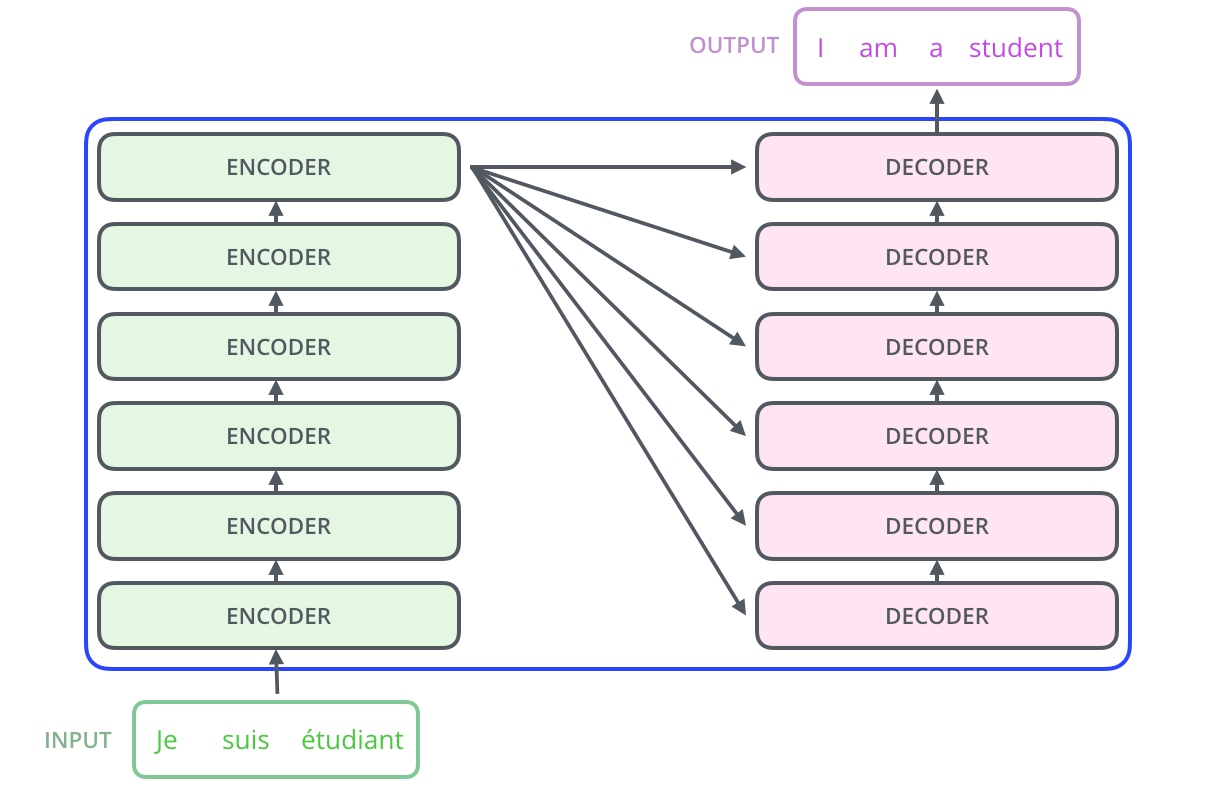
\includegraphics[scale=0.25]{imagenes/transformer.png}}  
    \caption{Transformer aplicado a la generación de texto \cite{transformers}}
    \label{fig:transformer}
\end{figure}

En cada codificador (Figura \ref{fig:encoder}), las características de entrada primero pasan por una capa de auto-atención, en la que interactúan entre sí y se descubre a cuáles hay que prestar mayor atención. La salida de esta primera capa serán los datos agregados resultantes de esas interacciones y las puntuaciones de atención. A continuación, se introduce esta salida en una red neuronal completamente conectada. \cite{self-attention}

Los decodificadores (Figura \ref{fig:decoder}) también poseen estas dos capas, pero entre ambas existe otra capa de atención que ayuda al decodificador a concentrarse en las características importantes de la entrada.

\begin{figure}[H]
\centering
    \begin{subfigure}{.85\textwidth}
        \centering
        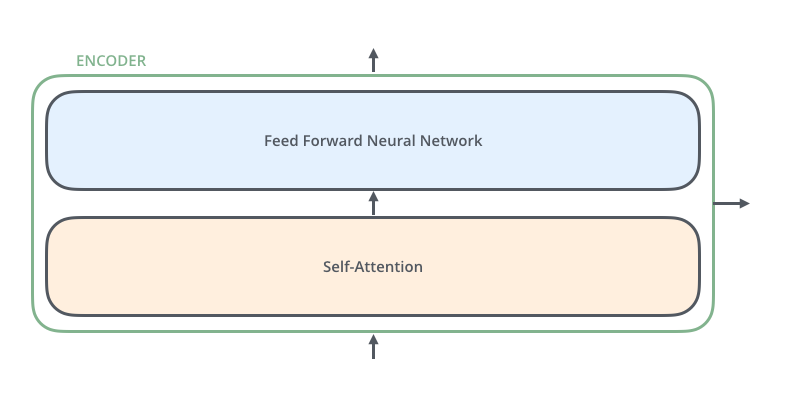
\includegraphics[width=1\linewidth]{imagenes/transformer_encoder.png}
        \caption{Estructura interior del codificador}
        \label{fig:encoder}
    \end{subfigure}%

    \bigskip

    \begin{subfigure}{.5\textwidth}
        \centering
        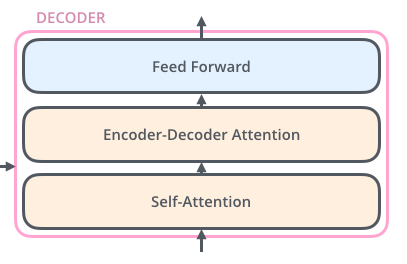
\includegraphics[width=1\linewidth]{imagenes/transformer_decoder.png}
        \caption{Estructura exterior del decodificador}
        \label{fig:decoder}
    \end{subfigure}

    \caption{Los dos tipos de capas que forman el Transformer \cite{transformers}}
\end{figure}


Los transformer son actualmente los modelos más efectivos en tareas como la generación de lenguaje natural, y también se han aplicado a generación de imágenes. Estos son capaces de memorizar datos de cualquier punto de la secuencia, al contrario que otros modelos recurrentes o convolutivos, que sólo almacenan las interacciones locales. \cite{transformers}



\newpage
\section{Bibliotecas y paquetes}
Existen productos desarrollados por investigadores que nos van a facilitar cumplir el objetivo del proyecto. 

\subsection{Taming Transformers for High-Resolution Image Synthesis} \label{taming-transformers}
Científicos de la Universidad de Heidelberg (Alemania) publicaron a finales de 2020 un modelo capaz de generar imágenes sintéticas de alta resolución utilizando transformers. En publicaciones previas ya se habían expuesto modelos generativos basados en transformers \cite{chen2020generative}, pero estos solo podían funcionar con imágenes de pequeño tamaño. El coste computacional de un transformer aplicado directamente en imágenes crece cuadráticamente con el tamaño de esta, así que no es viable utilizarlos en imágenes de más de 100x100 píxeles, y mucho menos en aquellas del orden del megapixel.

P. Esser et al. \cite{esser2021taming} desarrolla un método capaz de combinar la potencia generativa de los transformers con la eficiencia que aportan las redes convolutivas, detallado en la Figura \ref{fig:taming-transformers}. 

\begin{figure}[H]
\centering
    \fbox{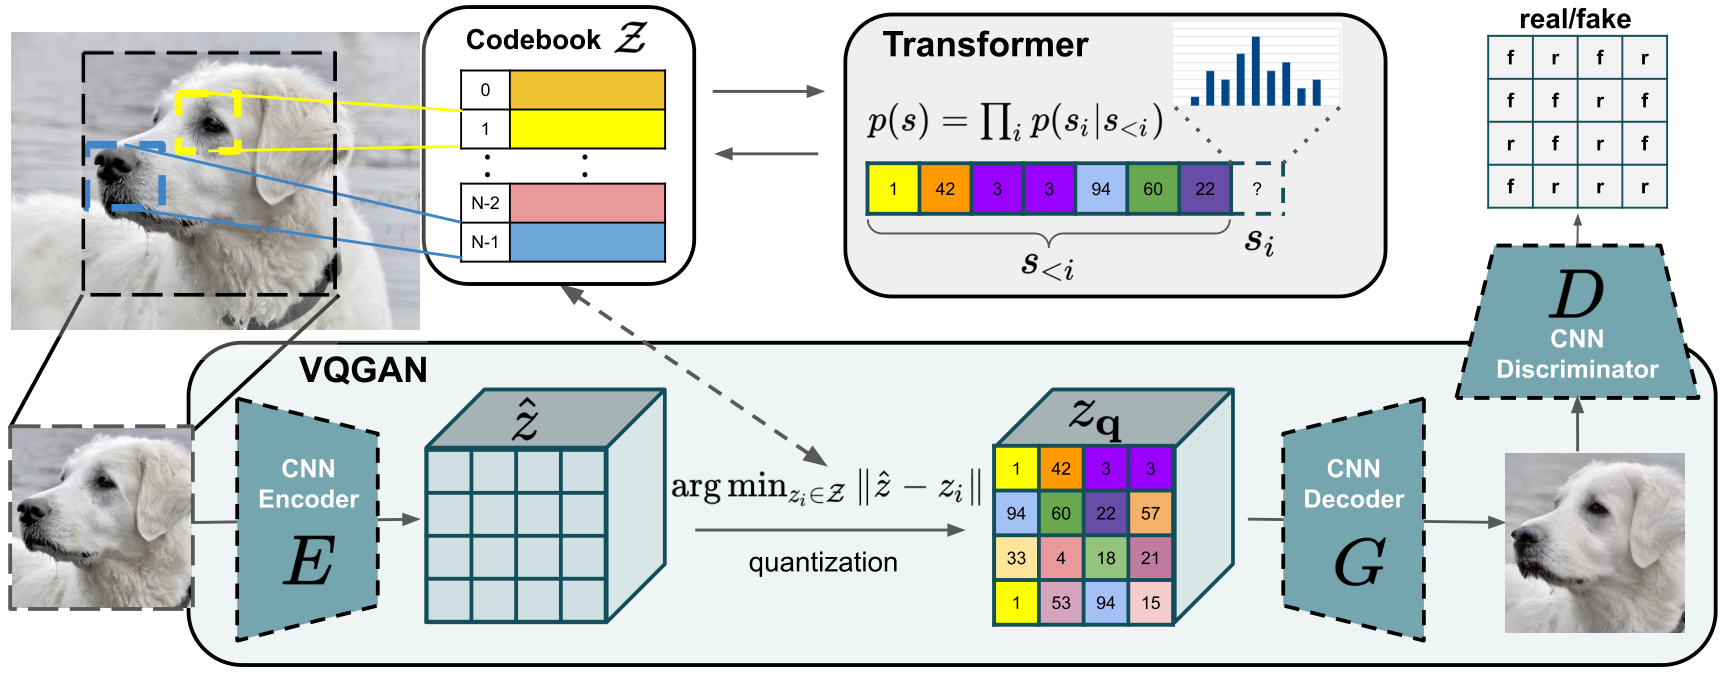
\includegraphics[scale=0.5]{imagenes/taming.png}}  
    \caption{Modelo propuesto por P. Esser et al. \cite{esser2021taming}}
    \label{fig:taming-transformers}
\end{figure}

La arquitectura convolutiva de la que hablo es un Vector Quantized Generative Adversarial Network (VQGAN), una variante de VQVAE propuesta por los autores de la publicación donde la estructura codificador-decodificador del VAE se entrena mediante un procedimiento adversarial, utilizando un discriminador.

Tras entrenar el modelo, se habrá generado un codebook que comprime la información de las imágenes. Será sobre este codebook sobre el que se entrene el transformer que posteriormente permitirá generar imágenes sintéticas. Ahora tendremos un modelo que es capaz de aprovechar la gran capacidad generativa de los transformers, manteniendo tiempos de entrenamiento razonables gracias a VQGAN.

La Figura \ref{fig:taming-examples} muestra los resultados que se pueden producir dada una imagen condicional de entrada.

\begin{figure}[H]
\centering
    \fbox{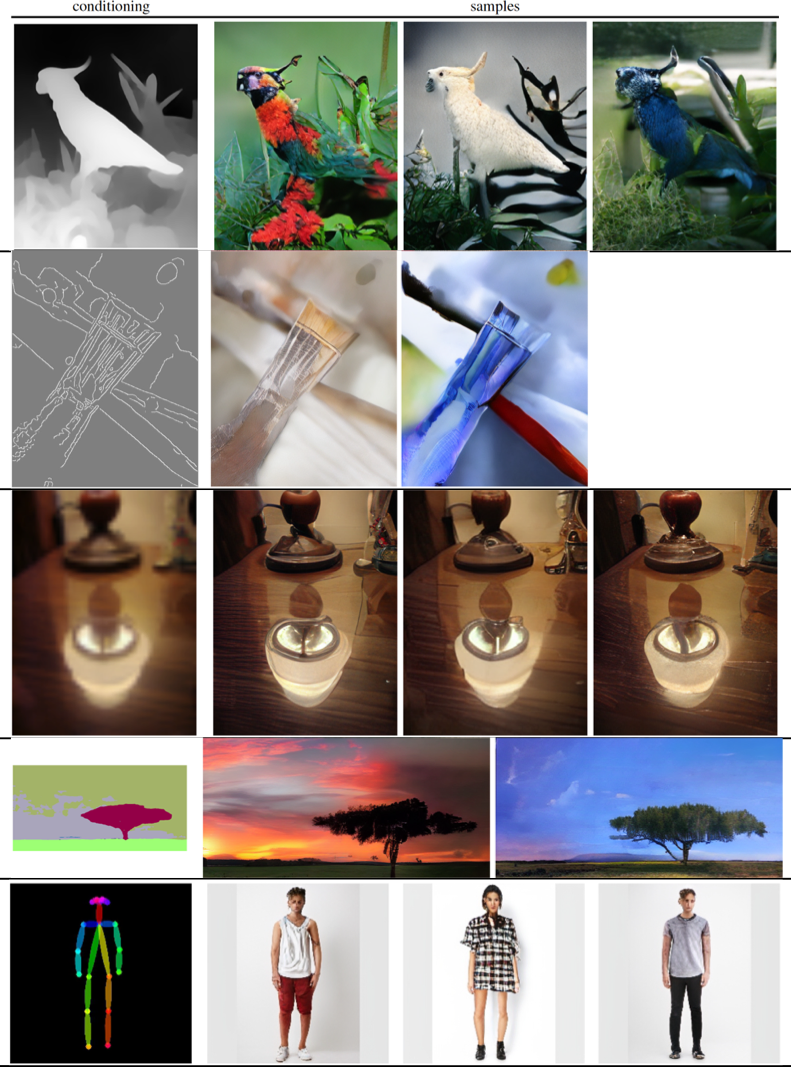
\includegraphics[scale=0.9]{imagenes/taming_examples.png}}  
    \caption{Ejemplos generados utilizando el modelo basado en transformer \cite{esser2021taming}}
    \label{fig:taming-examples}
\end{figure}

Se observa que funciona correctamente en diversas situaciones, por lo que puede ser una buena opción para nuestra la de síntesis de imágenes.

\subsection{Pytorch} \label{pytorch} 
PyTorch es una biblioteca basada en tensores optimizada para crear modelos de aprendizaje profundo que se entrenen y ejecuten tanto en GPUs como en CPUs.

\begin{figure}[H]
\centering
    \fbox{
\includegraphics[scale=0.2]{imagenes/pytorch.jpeg}}  
    \caption{Logo de PyTorch}
\end{figure}

Es adecuada para ser utilizada en proyectos de investigación, ya que convierte el desarrollar y experimentar con nuevas arquitecturas en algo relativamente sencillo. Su núcleo proporciona la capacidad de definir funciones matemáticas y calcular sus gradientes.

Al compararla con otras bibliotecas de aprendizaje profundo como Tensorflow encontramos diferencias. Esta sigue el paradigma definición-compilación-ejecución, mientras que PyTorch presenta una estructura definición-ejecución, donde no existe una etapa de compilación. El usuario puede definir una expresión matemática y calcular su gradiente directamente. \cite{ketkar2017introduction}

A continuación, voy a comentar algunas características y módulos incluidos en esta biblioteca que merece la pena conocer.

\subsubsection{Dataset y DataLoader}
El código para gestionar los datos con los que se trabaja se puede volver complejo y difícil de mantener. PyTorch proporciona los módulos $torch.utils.data.DataLoader$ y $torch.utils.data.Dataset$ para automatizar la carga y la manipulación de los datos, tanto procedentes de \textit{datasets} ya existentes (por ejemplo, MNIST) como de datos propios.

$torch.utils.data.Dataset$ es una clase heredada por una clase hija en la que se implementan ciertos métodos encargados de cargar los datos. Un dataset puede ser de tipo $iterable$ o de tipo $map$: los primeros implementan $\_\_iter\_\_()$, y permiten que el objeto sea iterable, de forma que $iter(dataset)$ devuelve un flujo de datos que están siendo leídos de una base de datos o incluso se están produciendo en tiempo real. Por otra parte, un \textit{dataset} de tipo $map$ implementa los métodos $\_\_getitem\_\_()$ y $\_\_len\_\_()$. Esto permite establecer una relación clave-dato, donde si $CompoundDataset$ es un \textit{dataset} con imágenes que pueden ser o no compuestos químicos, $CompoundDataset[idx]$ devolvería la imagen número $idx$ junto a su etiqueta. Este último tipo de \textit{dataset} es el que se utiliza en este proyecto.

El constructor de un objeto de tipo $torch.utils.data.DataLoader$ recibe como principal argumento un objeto $torch.utils.data.Dataset$. También recibe otros parámetros, como el tamaño del batch o si queremos que los datos sean devueltos en un orden aleatorio. Devuelve un iterable que cumple estas características, lo que facilita en gran medida el entrenamiento de modelos. 

Utilizando estos módulos se separan los datos del código de entrenamiento, obteniendo una mayor modularidad y un código más fácil de leer. \cite{pytorch-doc}

\subsubsection{Módulos $torch.nn$ y $torch.optim$}
El primero contiene los principales componentes utilizados en la construcción de redes neuronales y otras arquitecturas de aprendizaje profundo. Algunos de estos son:

\begin{itemize}
    \item \textbf{torch.nn.Module:} Es la clase padre de la que heredan todas las implementaciones de redes neuronales. En su constructor, entre otros elementos, se pueden inicializar diferentes capas que serán utilizadas en el método $forward()$, donde se especifica la estructura de la red y las conexiones entre ellas.
    \item \textbf{torch.nn.functional:} Recoge funciones de activación, de error así como capas de la red que no tienen un estado asociado.
    \item \textbf{torch.nn.Conv2d}, \textbf{torch.nn.MaxPool2d}, \textbf{torch.nn.Linear} son ejemplos de capas contenidas en este módulo. Existen diferentes tipos de capas lineales, convolutivas, recurrentes, transformer, etc. previamente implementadas y listas para ser utilizadas.
\end{itemize}

Por otro lado, $torch.optim$ contiene optimizadores como son SGD o Adam, encargados de actualizar los parámetros del modelo durante el entrenamiento. \cite{pytorch-doc}

\subsubsection{Autograd}
Al entrenar redes neuronales, el método más utilizado para actualizar los parámetros del modelo es la propagación hacia atrás o \textit{back propagation}. Estos se ajustan de acuerdo al gradiente de la función de error con respecto al parámetro dado.

PyTorch facilita la aplicación de la propagación hacia atrás a través del módulo $torch.autograd$. Cuando se implementa un modelo, solo es necesario declarar el método $forward()$, ya que PyTorch crea sobre la marcha el grafo de las operaciones necesarias para calcular el gradiente. Durante el entrenamiento del modelo, al llamar a $loss.backward()$ se calculará el gradiente utilizando este grafo. \cite{pytorch-doc}

Como conclusión, PyTorch aporta una gran flexibilidad para crear modelos de aprendizaje profundo, su sintaxis y paradigma de programación son relativamente fáciles de aprender y contiene un gran número de módulos que permiten crear modelos complejos. Aparte, es compatible con el entrenamiento en GPU y permite guardar los modelos entrenados. Por todas estas razones puede resultar una librería adecuada para implementar el clasificador de imágenes.

\chapter{Metodología}

En esta sección explicamos en la metodología de investigación seguida para lograr desarrollar un producto válido para los científicos Israelíes. Hemos partido de un dataset facilitado por ellos, que hemos utilizado para entrenar un modelo que genera imágenes sintéticas y para implementar un clasificador de imágenes.

Toda la implementación se encuentra en el repositorio de GitHub del proyecto \cite{repository}. La raíz del repositorio contiene los siguientes elementos:

\dirtree{%
    .1 /.
    .2 datasets/.
    .2 experiments/\DTcomment{implementación del TFG}.
    .2 papers/\DTcomment{algunas de las publicaciones utilizadas en su desarrollo}.
    .2 report/\DTcomment{memoria en formato \LaTeX}.
    .2 slides/.
    .2 README.md.
}

En el repositorio, el directorio datasets se encuentra vacío para no crear problemas con el sistema de control de versiones. En el README.md se indica un enlace donde se pueden descargar los datos que se deben colocar en el directorio.

\newpage
\section{Dataset utilizado}
El dataset contiene ejemplos positivos y negativos. Todas las imágenes son diferentes, presentan elementos con distintos trazados de línea, tamaños, colores... Originalmente se encuentran en formato .png.

Los ejemplos positivos son imágenes de moléculas extraídas de publicaciones. La mayoría son moléculas completas, aunque algunas parecen recortes de estructuras más grandes. En total tenemos 162 imágenes de este tipo.

\begin{figure}[H]
\centering
    \fbox{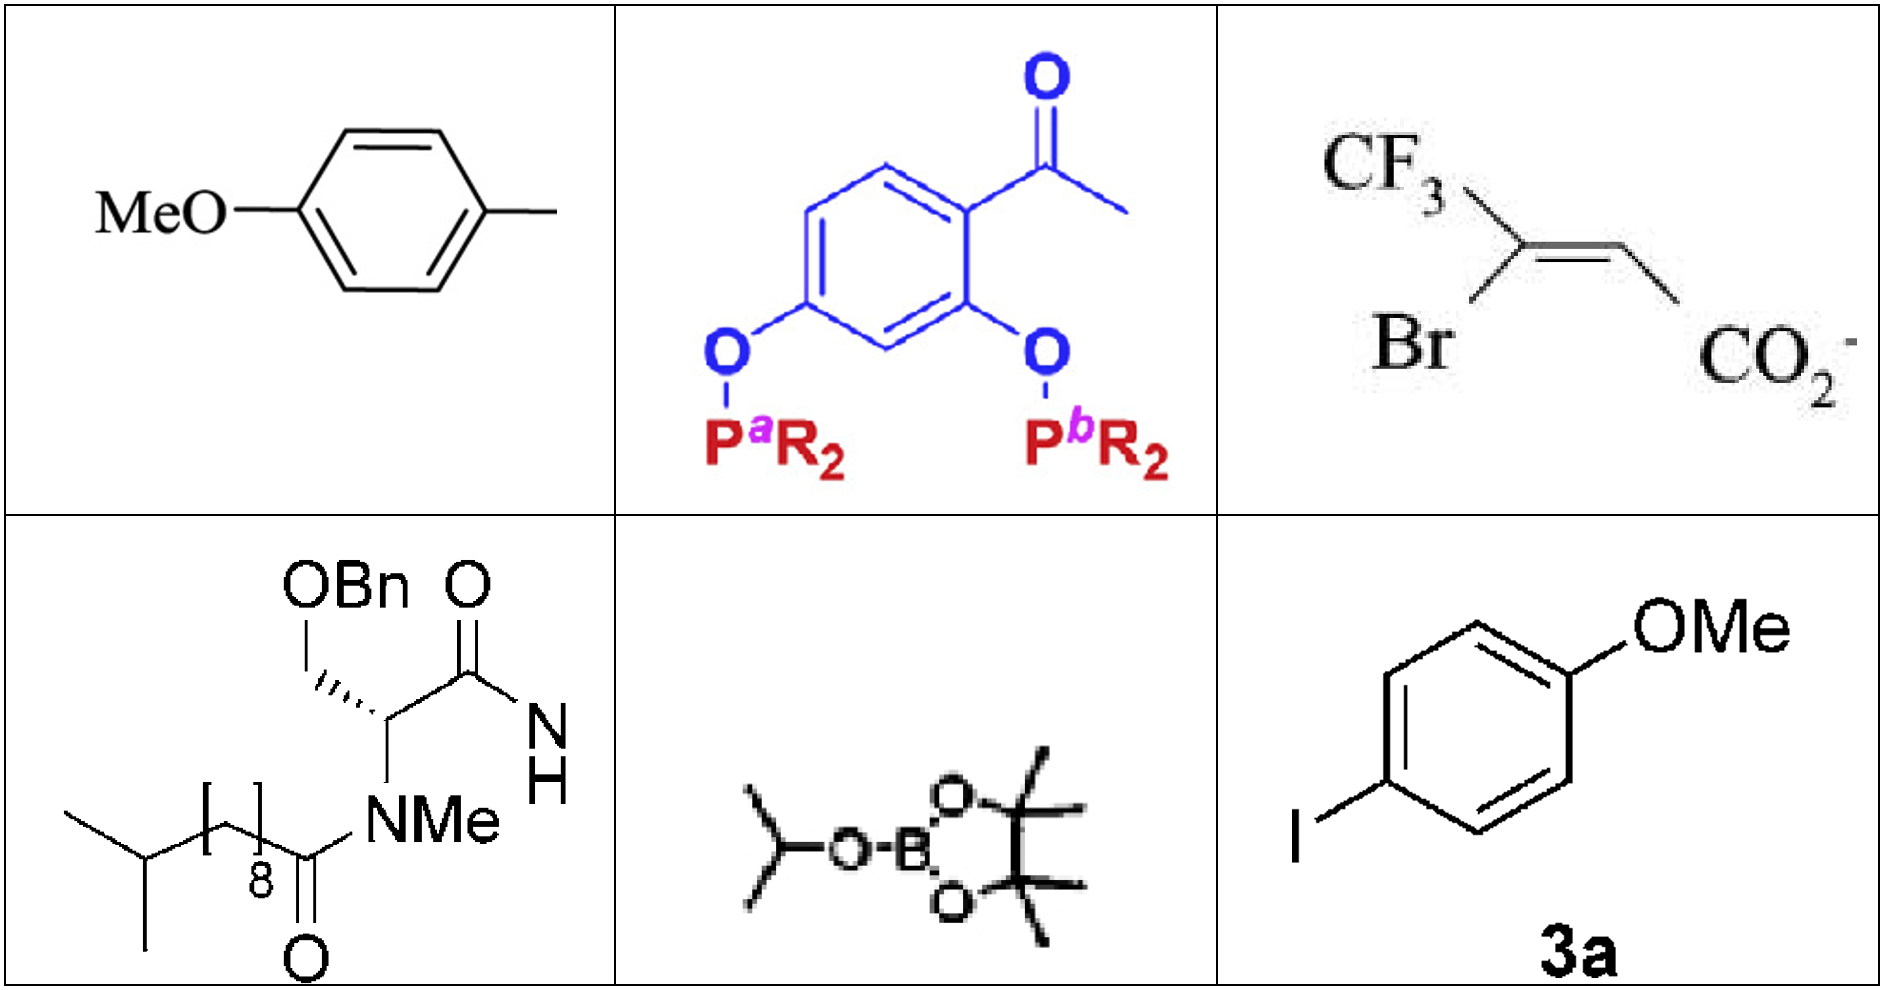
\includegraphics[scale=0.3]{imagenes/positive_examples.png}}  
    \caption{Ejemplos de muestras positivas del dataset} 
\end{figure}

Los ejemplos negativos son, en cambio, imágenes que contienen rectas, curvas y otras figuras que se parecen a las formas que adquiere una molécula, pero no lo son. En esta categoría hay más imágenes, 800 en total.

\begin{figure}[H]
\centering
    \fbox{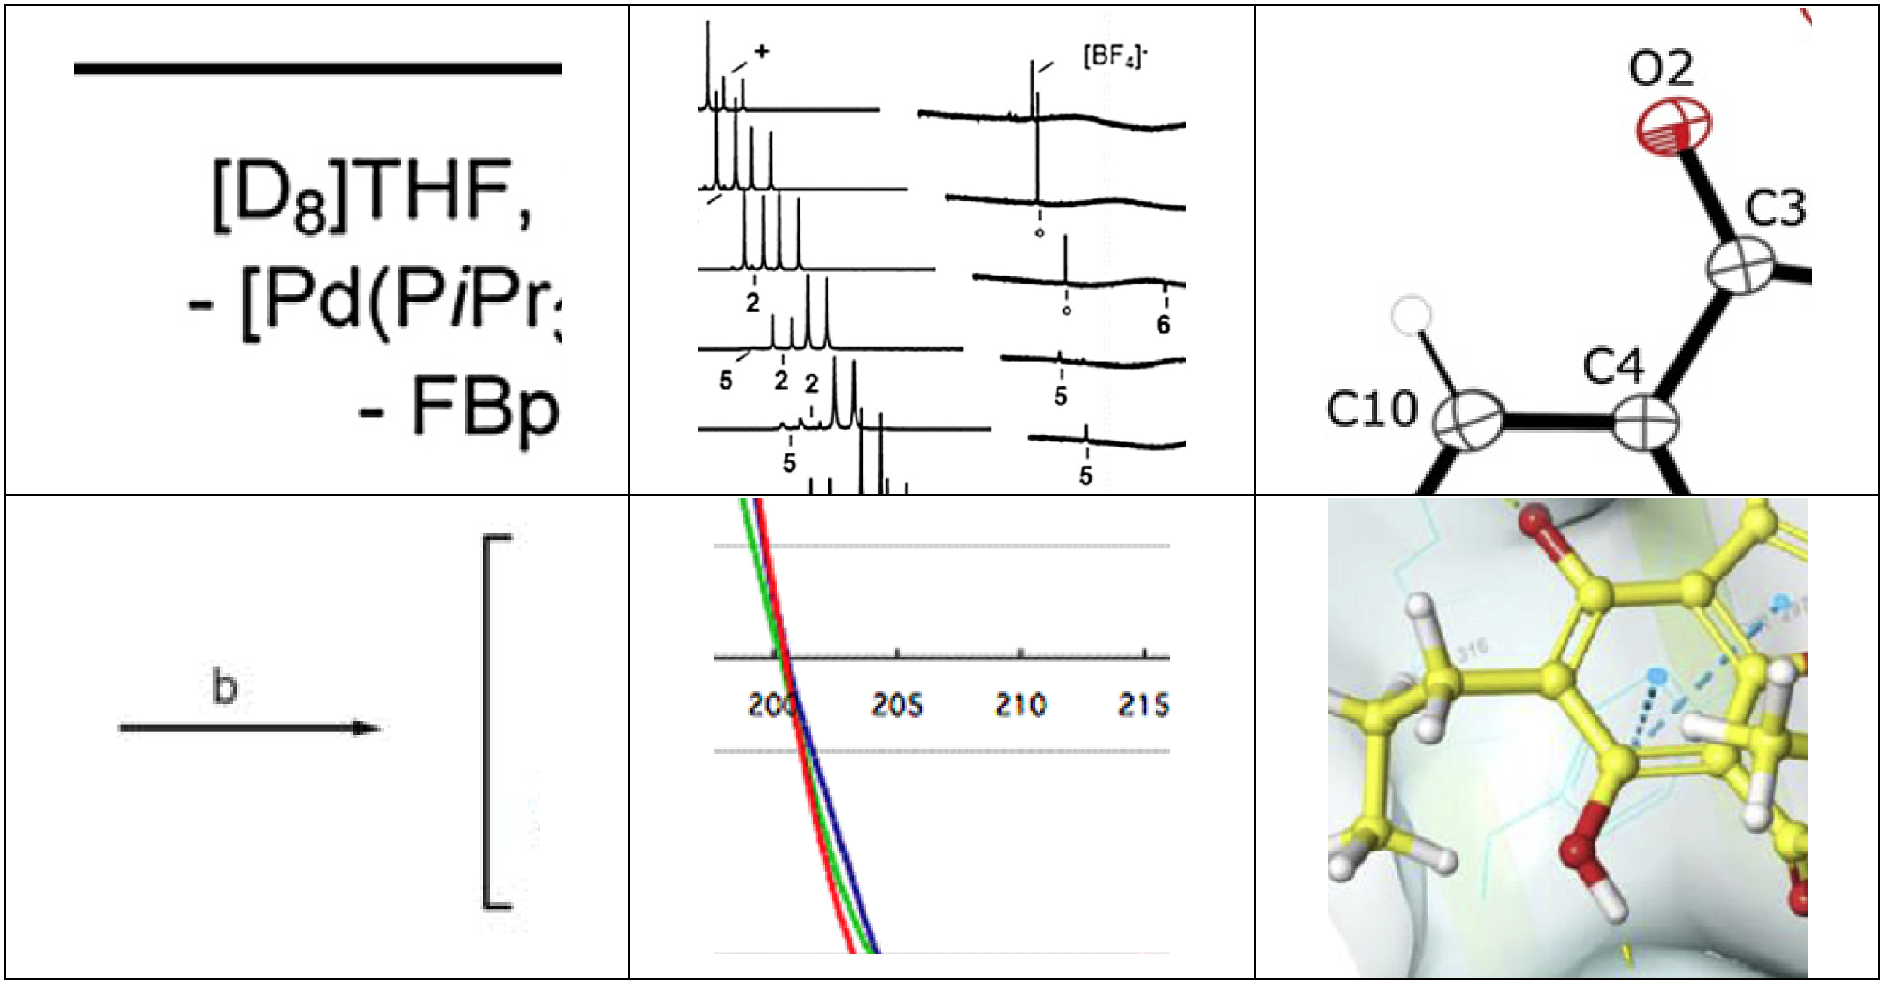
\includegraphics[scale=0.3]{imagenes/negative_examples.png}}  
    \caption{Ejemplos de muestras negativas del dataset} 
\end{figure}

Estas imágenes necesitan un preprocesamiento, es necesario elegir el formato con el que se va a trabajar y dimensionarlas para que todas tengan el mismo tamaño. Debido a que el canal alfa del formato .png no se está aprovechando, decidimos convertirlas a formato .jpg y así trabajar con tres canales en nuestros modelos. Además, el modelo generativo que utilizamos está diseñado para trabajar con imágenes con este número de canales, así que será lo más adecuado.

Lo más conveniente sería dimensionar todas las imágenes al tamaño de la más grande, así no se perdería información. Pero esto puede suponer un problema, ya que existen algunas que superan los 700x700 píxeles, y cuanto mayor es su resolución más parámetros necesitan almacenar los modelos, dando lugar a altos tiempos de ejecución, y sobre todo, a problemas con la memoria de la GPU. Las GPUs del clúster no tienen capacidad para almacenar modelos con tantos parámetros, por lo que decidimos reducir el tamaño de las imágenes a 256x256. 

También mencionar el limitado número de ejemplos positivos que tenemos en comparación con negativos: estamos ante un conjunto de datos desbalanceado. En el momento de entrenar el clasificador, tendremos que conseguir que esté balanceado, ya sea reduciendo el número de ejemplos negativos utilizado o aplicando \textit{data augmentation} sobre los positivos. En este trabajo elegimos la segunda opción, ya que en Aprendizaje Automático cuantos más datos se utilizan en el entrenamiento, mejores modelos se obtienen y con mayor capacidad de generalización. 

La técnica de \textit{data augmentation} consiste en aumentar el tamaño del conjunto de datos completándolo con imágenes alteradas de este. Existen bibliotecas en lenguajes de programación como Python que facilitan en gran medida esta tarea, ya que permiten indicar, entre una serie de transformaciones ya implementadas, cuáles queremos aplicar \cite{imgaug}. En nuestro caso vamos a crear tres \textit{data augmentation} diferentes, y comprobaremos cuál funciona mejor en los experimentos. La primera realizará transformaciones suaves, la segunda algo más fuertes y la tercera bastante disruptivas.

\begin{algorithm}[H]
    \caption{\textit{Data augmentation} 1: Transformaciones suaves}
\begin{algorithmic}[1]
    \State A\_veces(50\%, DesenfoqueGaussiano(sigma=[0, 0.5]))
    \State Escalar(x: [80\%, 100\%], y: [80\%, 100\%])
    \State Rotar([-25º, +25º])
    \State Estirar([-5,5])
\end{algorithmic}
\end{algorithm}

A cada imagen del conjunto de datos se le aplicarán estas cuatro transformaciones, la primera solamente con un 50\% de probabilidad. Los parámetros de cada transformación vienen dados en un rango, de forma que se elige un valor aleatorio en este.

\begin{figure}[H]
\centering
    \begin{subfigure}{.35\textwidth}
        \centering
        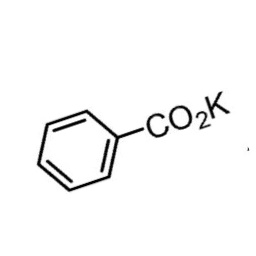
\includegraphics[width=1\linewidth]{imagenes/aug/180.jpg}
    \end{subfigure}%
    \begin{subfigure}{.35\textwidth}
        \centering
        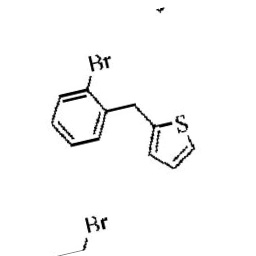
\includegraphics[width=1\linewidth]{imagenes/aug/193.jpg}
    \end{subfigure}%

    \bigskip

    \begin{subfigure}{.35\textwidth}
        \centering
        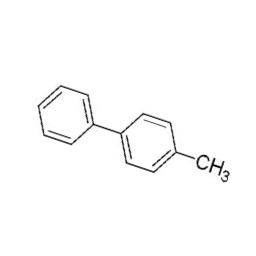
\includegraphics[width=1\linewidth]{imagenes/aug/224.jpg}
    \end{subfigure}%
    \begin{subfigure}{.35\textwidth}
        \centering
        
\includegraphics[width=1\linewidth]{imagenes/aug/370.jpg}
    \end{subfigure}

    \caption{Imágenes generadas aplicando \textit{data augmentation} 1}
\end{figure}

Algunos ejemplos son los que se muestran sobre este párrafo, se aprecian leves rotaciones y estiramientos de las imágenes, sin existir gran diferencia con las originales.

\begin{algorithm}[H]
    \caption{\textit{Data augmentation} 2: Transformaciones más fuertes}
\begin{algorithmic}[1]
    \State A\_veces(50\%, DesenfoqueGaussiano(sigma=[0, 0.5]))
    \State ContrasteLineal([0.75, 1.5])
    \State Escalar(x: [70\%, 100\%], y: [70\%, 100\%])
    \State Rotar([-45º, +45º])
    \State Estirar([-10,10])
    \State Trasladar(x: [-10\%, 10\%], y: [-10\%, 10\%])
    \State Multiplicar([0.8, 1.2], por\_canal=25\%)
    \State RuidoGaussianoAditivo(loc=0, escala=[0.0, 0.05*255])
    \State VoltearIzdaDcha(30\%)
\end{algorithmic}
\end{algorithm}

En este caso, utilizaremos transformaciones como Multiplicar (multiplica el valor de los píxeles de la imagen por un número entre 0.8 y 1.2), RuidoGaussianoAditivo (donde a cada píxel se le añade ruido generado mediante una distribución gaussiana centrada en 0 y con desviación entre 0 y 0.05*255) o VoltearIzqdaDcha, entre otras.

\begin{figure}[H]
\centering
    \begin{subfigure}{.35\textwidth}
        \centering
        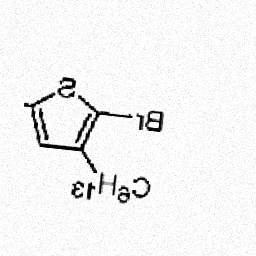
\includegraphics[width=1\linewidth]{imagenes/aug2/169.jpg}
    \end{subfigure}%
    \begin{subfigure}{.35\textwidth}
        \centering
        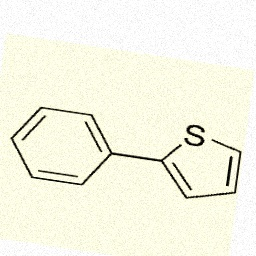
\includegraphics[width=1\linewidth]{imagenes/aug2/188.jpg}
    \end{subfigure}%

    \bigskip

    \begin{subfigure}{.35\textwidth}
        \centering
        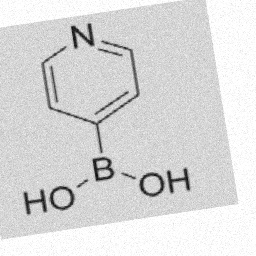
\includegraphics[width=1\linewidth]{imagenes/aug2/221.jpg}
    \end{subfigure}%
    \begin{subfigure}{.35\textwidth}
        \centering
        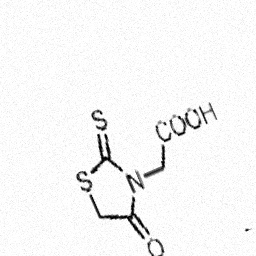
\includegraphics[width=1\linewidth]{imagenes/aug2/222.jpg}
    \end{subfigure}

    \caption{Imágenes generadas aplicando \textit{data augmentation} 2}
\end{figure}

En este caso se observan más cambios fundamentalmente debidos a las variaciones en contraste, al uso de ruido gaussiano y a la multiplicación, responsable de los cambios de color, ya que a veces se aplica a canales independientes. 

\begin{algorithm}[H]
    \caption{\textit{Data augmentation} 3: Transformaciones fuertes}
\begin{algorithmic}[1]
    \State A\_veces(50\%, DesenfoqueGaussiano(sigma=[0, 0.6]))
    \State ContrasteLineal([0.75, 2])
    \State Escalar(x: [70\%, 100\%], y: [70\%, 100\%])
    \State Rotar([-45º, +45º])
    \State Estirar([-10,10])
    \State Trasladar(x: [-20\%, 20\%], y: [-10\%, 10\%])
    \State Multiplicar([0.6, 1.4], por\_canal=25\%)
    \State RuidoGaussianoAditivo(loc=0, escala=[0.0, 0.05*255], por\_canal=30\%)
    \State VoltearIzdaDcha(20\%)
    \State VoldearArribaAbajo(20\%)
    \State A\_veces(70\%, TransformacionElastica(alfa=[0.75, 3], sigma=(0.2, 0.5)))
    \State UnoEntre(Nitidez(alfa=[0, 1], lightness=[0.5, 1.5]), Emboss(alfa=[0, 1], fuerza=[0.75, 2]))
    \State Dropout([0.01, 0.15], por\_canal=0.5)
\end{algorithmic}
\end{algorithm}
% TODO: Cómo se traduce emboss al español??

Finalmente, en esta versión de \textit{data augmentation} añadimos transformaciones que alteran en gran medida el aspecto de las imágenes. TransformacionElastica desplaza píxeles de una zona de la imagen a otra cercana, donde alfa controla la distancia con la que se produce el desplazamiento y sigma la suavidad de este, un valor bajo de sigma dará lugar a imágenes ruidosas y pixeladas. Nitidez aplica este efecto a la imagen y mezcla el resultado con la imagen original, la intensidad de la mezcla se controla con el parámetro alfa, mientras que el parámetro lightness controla el brillo de la imagen. Emboss da a la imagen un aspecto metálico, pronunciando las altas luces y sombras. Por último, Dropout da el valor 0 a cada pixel con una probabilidad entre 0.01 y 0.15. 

\begin{figure}[H]
\centering
    \begin{subfigure}{.35\textwidth}
        \centering
        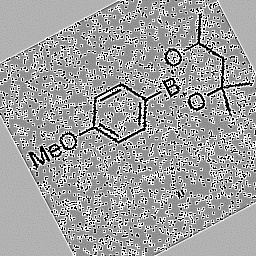
\includegraphics[width=1\linewidth]{imagenes/aug3/175.jpg}
    \end{subfigure}%
    \begin{subfigure}{.35\textwidth}
        \centering
        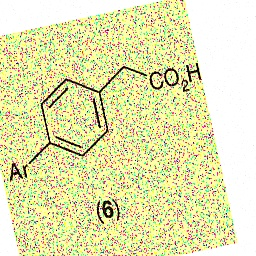
\includegraphics[width=1\linewidth]{imagenes/aug3/183.jpg}
    \end{subfigure}%

    \bigskip

    \begin{subfigure}{.35\textwidth}
        \centering
        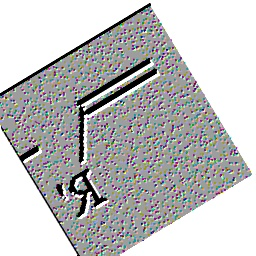
\includegraphics[width=1\linewidth]{imagenes/aug3/225.jpg}
    \end{subfigure}%
    \begin{subfigure}{.35\textwidth}
        \centering
        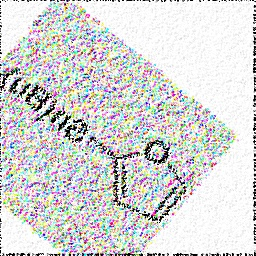
\includegraphics[width=1\linewidth]{imagenes/aug3/271.jpg}
    \end{subfigure}

    \caption{Imágenes generadas aplicando \textit{data augmentation} 3}
\end{figure}

En esta última versión las transformaciones son bastante agresivas. Se introduce mucho ruido en las imágenes y las rotaciones y los cambios en el contraste son fuertes.

\section{Estructura del código}
Como se menciona al principio del capítulo, la implementación se sitúa en el directorio $experiments/$, dividido en dos subdirectorios. El primero contiene el código del modelo generador de imágenes, el segundo el del clasificador: \\

\dirtree{%
    .1 experiments/\DTcomment{implementación del TFG}.
    .2 taming\_transformers/\DTcomment{generador de imágenes}.
    .3 taming-transformers/.
    .4 configs/.
    .4 logs/.
    .4 train\_ngpu.sh.
    .3 data\_generation\_and\_aug.ipynb.
    .3 sample\_and\_clean\_molecules.ipynb.
    .3 sampling\_experiment.ipynb.
    .3 functions.py.
    .2 image\_classifier/\DTcomment{clasificador de imágenes}.
    .3 saved\_models/.
    .3 datasets.py.
    .3 functions.py.
    .3 grid\_search.py.
    .3 models.py.
    .3 train.py.
    .3 train\_ngpu.sh.
}

\subsection{Generador de imágenes sintéticas}
Uno de los objetivos del proyecto es construir un modelo que nos permita generar imágenes sintéticas de moléculas. 

\section{Ejecución y reproducibilidad}
Como ejecutar los scripts y semillas utilizadas

\chapter{Experimentación}
En esta sección se explican los experimentos realizados hasta alcanzar la versión final del clasificador siguiendo los pasos propuestos en la metodología. Delimitar las pruebas que se van a realizar en un proyecto es fundamental para concentrar los esfuerzos y cumplir con los objetivos en plazo. Al tratarse de un proyecto de investigación, realizo experimentos iniciales, evalúo los resultados y vuelvo a realizar experimentos hasta alcanzar unos resultados que cumplan con los objetivos.

La implementación de los experimentos realizados se encuentra en el repositorio de GitHub del proyecto \cite{repository}. La raíz del repositorio contiene los siguientes elementos:

\dirtree{%
    .1 /.
    .2 datasets/.
    .2 experiments/\DTcomment{implementación del TFG}.
    .2 papers/\DTcomment{algunas de las publicaciones utilizadas en su desarrollo}.
    .2 report/\DTcomment{memoria en formato \LaTeX}.
    .2 slides/.
    .2 README.md.
}

\newpage
\section{Transformaciones sobre el \textit{dataset}}
Tras recibir el \textit{dataset} y normalizar el tamaño de las imágenes, procedo a aplicar las tres secuencias de \textit{data augmentation} que he explicado en el capítulo anterior.

El \textit{dataset} original y los derivados obtenidos al aplicar \textit{data augmentation} se almacenarán en el directorio \textit{datasets/} del repositorio, como se describe en el siguiente árbol:

\vspace{0.2cm}
\dirtree{%
    .1 datasets/.
    .2 negev/.
    .3 articles\_molecules/\DTcomment{ejemplos positivos}.
    .4 preprocess256/\DTcomment{imágenes 256x256}.
    .5 aug/\DTcomment{\textit{data augmentation} 1}. 
    .6 1.png.
    .6 2.png.
    .6 \ldots.
    .5 aug2/\DTcomment{\textit{data augmentation} 2}.
    .6 1.png.
    .6 2.png.
    .6 \ldots.
    .5 aug3/\DTcomment{\textit{data augmentation} 3}.
    .6 1.png.
    .6 2.png.
    .6 \ldots.
    .5 1.png.
    .5 2.png.
    .5 \ldots.
    .4 1.png.
    .4 2.png.
    .4 \ldots.
    .3 not\_molecules/\DTcomment{ejemplos negativos}.
}

El código que me permitirá realizar estas transformaciones se encuentra en los siguientes archivos:

\vspace{0.2cm}
\dirtree{%
    .1 experiments/.
    .2 taming\_transformers/.
    .3 data\_generation\_and\_augmentation.ipynb.
    .3 functions.py.
}

\noindent \textit{{data\_generation\_and\_augmentation.ipynb}} contiene el código que pre-procesa las imágenes, transformándolas de forma que tengan el mismo tamaño, y que aplica las tres secuencias de \textit{data augmentation} que he comentado.

\noindent \textit{functions.py} declara funciones utilizadas por todos este cuaderno.

\noindent Aunque no se mencionan aquí, existen otros directorios y ficheros auxiliares que permiten funcionar a estos.

Comienzo por \textit{data augmentation} 1. Al aplicarla se obtienen los resultados mostrados en la Figura \ref{fig:data-aug1}.

\begin{figure}[H]
\centering
    \begin{subfigure}{.25\textwidth}
        \centering
        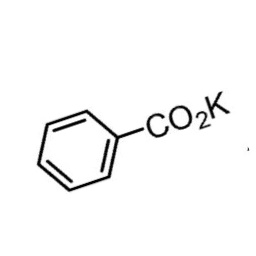
\includegraphics[width=1\linewidth]{imagenes/aug/180.jpg}
    \end{subfigure}%
    \begin{subfigure}{.25\textwidth}
        \centering
        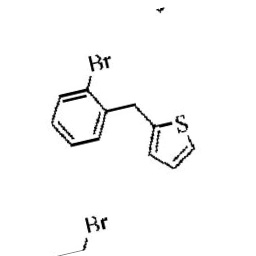
\includegraphics[width=1\linewidth]{imagenes/aug/193.jpg}
    \end{subfigure}%

    \bigskip

    \begin{subfigure}{.25\textwidth}
        \centering
        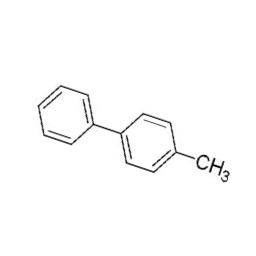
\includegraphics[width=1\linewidth]{imagenes/aug/224.jpg}
    \end{subfigure}%
    \begin{subfigure}{.25\textwidth}
        \centering
        
\includegraphics[width=1\linewidth]{imagenes/aug/370.jpg}
    \end{subfigure}

    \caption{Imágenes generadas aplicando \textit{data augmentation} 1}
    \label{fig:data-aug1}
\end{figure}

Se aprecian leves rotaciones y estiramientos de las imágenes, sin existir gran diferencia con las originales. Al estar aplicando tres veces la transformación sobre el conjunto de datos, puede que los cambios sean demasiado suaves dando lugar a imágenes muy similares. A continuación, observemos los resultados de \textit{data augmentation} 2 en la Figura \ref{fig:data-aug2}.

\begin{figure}[H]
\centering
    \begin{subfigure}{.23\textwidth}
        \centering
        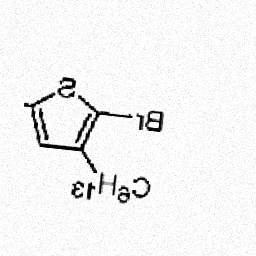
\includegraphics[width=1\linewidth]{imagenes/aug2/169.jpg}
    \end{subfigure}%
    \begin{subfigure}{.23\textwidth}
        \centering
        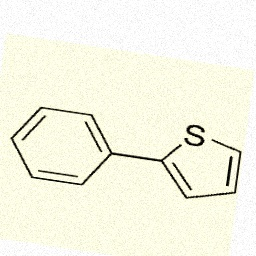
\includegraphics[width=1\linewidth]{imagenes/aug2/188.jpg}
    \end{subfigure}%

    \bigskip

    \begin{subfigure}{.23\textwidth}
        \centering
        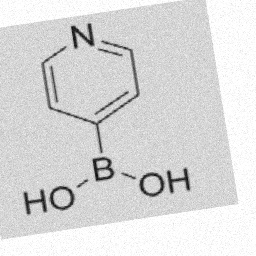
\includegraphics[width=1\linewidth]{imagenes/aug2/221.jpg}
    \end{subfigure}%
    \begin{subfigure}{.23\textwidth}
        \centering
        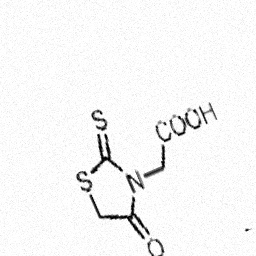
\includegraphics[width=1\linewidth]{imagenes/aug2/222.jpg}
    \end{subfigure}

    \caption{Imágenes generadas aplicando \textit{data augmentation} 2}
    \label{fig:data-aug2}
\end{figure}

En este caso se observan más cambios fundamentalmente debidos a las variaciones en contraste, al uso de ruido gaussiano y a la multiplicación, responsable de los cambios de color, ya que a veces se aplica a canales independientes. Puede ser una transformación adecuada, ya que añade diversidad al conjunto sin cambios demasiado pronunciados. 

Por último, comprobemos los resultados que se obtienen al aplicar \textit{data augmentation} 3 en la Figura \ref{fig:data-aug3}.

\begin{figure}[H]
\centering
    \begin{subfigure}{.23\textwidth}
        \centering
        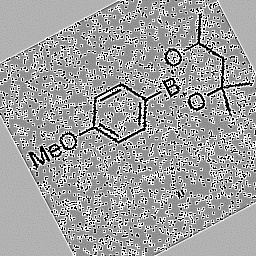
\includegraphics[width=1\linewidth]{imagenes/aug3/175.jpg}
    \end{subfigure}%
    \begin{subfigure}{.23\textwidth}
        \centering
        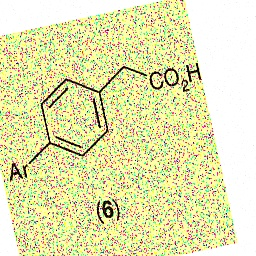
\includegraphics[width=1\linewidth]{imagenes/aug3/183.jpg}
    \end{subfigure}%

    \bigskip

    \begin{subfigure}{.23\textwidth}
        \centering
        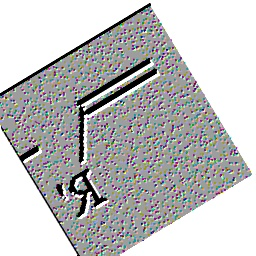
\includegraphics[width=1\linewidth]{imagenes/aug3/225.jpg}
    \end{subfigure}%
    \begin{subfigure}{.23\textwidth}
        \centering
        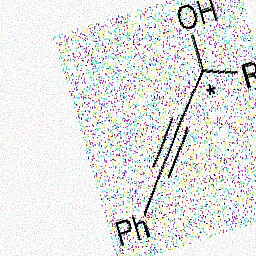
\includegraphics[width=1\linewidth]{imagenes/aug3/347.jpg}
    \end{subfigure}

    \caption{Imágenes generadas aplicando \textit{data augmentation} 3}
    \label{fig:data-aug3}
\end{figure}

En esta última versión las transformaciones son bastante agresivas. Se introduce mucho ruido en las imágenes y las rotaciones y los cambios en el contraste son fuertes.

Para entrenar el clasificador, seguramente las imágenes más adecuadas sean las generadas por \textit{data augmentation} 2. Son las más equilibradas, ya que la versión 1 apenas introduce cambios y la versión 3 añade demasiado ruido, creando imágenes que no se corresponden con la realidad y por tanto pueden penalizar el rendimiento del modelo.

\newpage
\section{Generación de imágenes sintéticas}

Sobre los cuatro conjuntos de datos se entrenarán modelos con diferente número de épocas, desde 70 hasta 170, aumentando de 20 en 20. De esta forma tendré $4 * |[70, 90, 110, 130, 150, 170]| = 4 * 6 = 24$ modelos diferentes.

Una vez entrenados, probaré a generar imágenes a partir de estos para ver cuál se comporta mejor. Para ello, debo introducirles algún tipo de imagen de entrada.

La generación de imágenes se va a realizar utilizando el modelo desarrollado por Esser et al. \cite{esser2021taming}, descrito en la Sección \label{st:taming-transformers}. El código en el que se realizan los experimentos con el generador se encuentra en los siguientes archivos:

\vspace{0.2cm}
\dirtree{%
    .1 experiments/\DTcomment{implementación del TFG}.
    .2 taming\_transformers/\DTcomment{generador de imágenes}.
    .3 taming-transformers/\DTcomment{implementación del generador}.
    .3 sample\_and\_clean\_molecules.ipynb.
    .3 sampling\_experiment.ipynb.
    .3 functions.py.
}

\noindent El subdirectorio \textit{taming-transformers/} contiene la implementación del modelo generativo proporcionada por sus autores \cite{taming-transformers-github}. 

\noindent \textit{sampling\_experiment.ipynb} es un cuaderno que, una vez entrenados los modelos, permite cargarlos y generar imágenes sintéticas a partir de otra imagen de entrada. Se utiliza para comprobar a partir de que \textit{dataset} se generan mejores resultados y con qué número de épocas. Es importante saber que este modelo generativo necesita de una imagen condicionante para generar una imagen sintética: se realizarán pruebas con distintos tipos, entre ellas ruido, para comprobar con cuáles se obtienen mejores resultados.

\noindent \textit{sample\_and\_clean\_molecules.ipynb}  permite generar un lote de imágenes sintéticas indicando el modelo que queremos utilizar y las propiedades del ruido, en concreto de ruido Perlín, ruido que explicaremos en los experimentos. También creará el \textit{dataset} final que contiene \textit{hard negatives}.

\noindent \textit{functions.py} declara funciones utilizadas por todos estos cuadernos.

\newpage
En las páginas siguientes se muestran los resultados. Cada fila corresponde a una imagen de entrada al modelo. En las columnas, la primera muestra la imagen de entrada mientras que cada una de las siguientes corresponde con un modelo entrenado durante x épocas, desde 70 hasta 170 (70, 90, 110, 130, 150, 170).

Se puede observar como la versión sin \textit{data augmentation} (Figura \ref{fig:synthetic_molecules}) no funciona bien, produce imágenes sin apenas estructura. Esto se debe a que solo se utilizan 162 imágenes, cifra muy baja para una arquitectura de deep learning como es un \textit{transformer}. Con \textit{data augmentation} (Figura \ref{fig:synthetic_molecules_aug1}) 1 tampoco se observan resultados de buena calidad, puede que algo mejores que en el caso anterior pero sin muchas diferencias.

Es en \textit{data augmentation} 2 (Figura \ref{fig:synthetic_molecules_aug2}) cuando ya se empiezan a ver mayores diferencias. El uso de transformaciones más fuertes crea un conjunto heterogéneo de imágenes y el modelo puede aprender más características de estas. Los resultados son aceptables, aunque el cambio de color que las transformaciones producían en algunas imágenes de entrenamiento ha dado lugar a fondos grisáceos en sus homólogas sintéticas. 

Con el tercer \textit{data augmentation} (Figura \ref{fig:synthetic_molecules_aug3}) estos fondos grisáceos son mucho más marcados. Recordar que estas transformaciones eran mucho más fuertes, por lo que se traslada a las imágenes sintéticas.


\begin{figure}[H]
\centering
    \caption{Resultados de entrenar los modelos sobre el conjunto de datos sin \textit{data augmentation}. La primera columna representa la imagen de entrada, el resto los diferentes modelos entrenados desde 70 hasta 170 épocas, tomadas de 20 en 20.} 
    \fbox{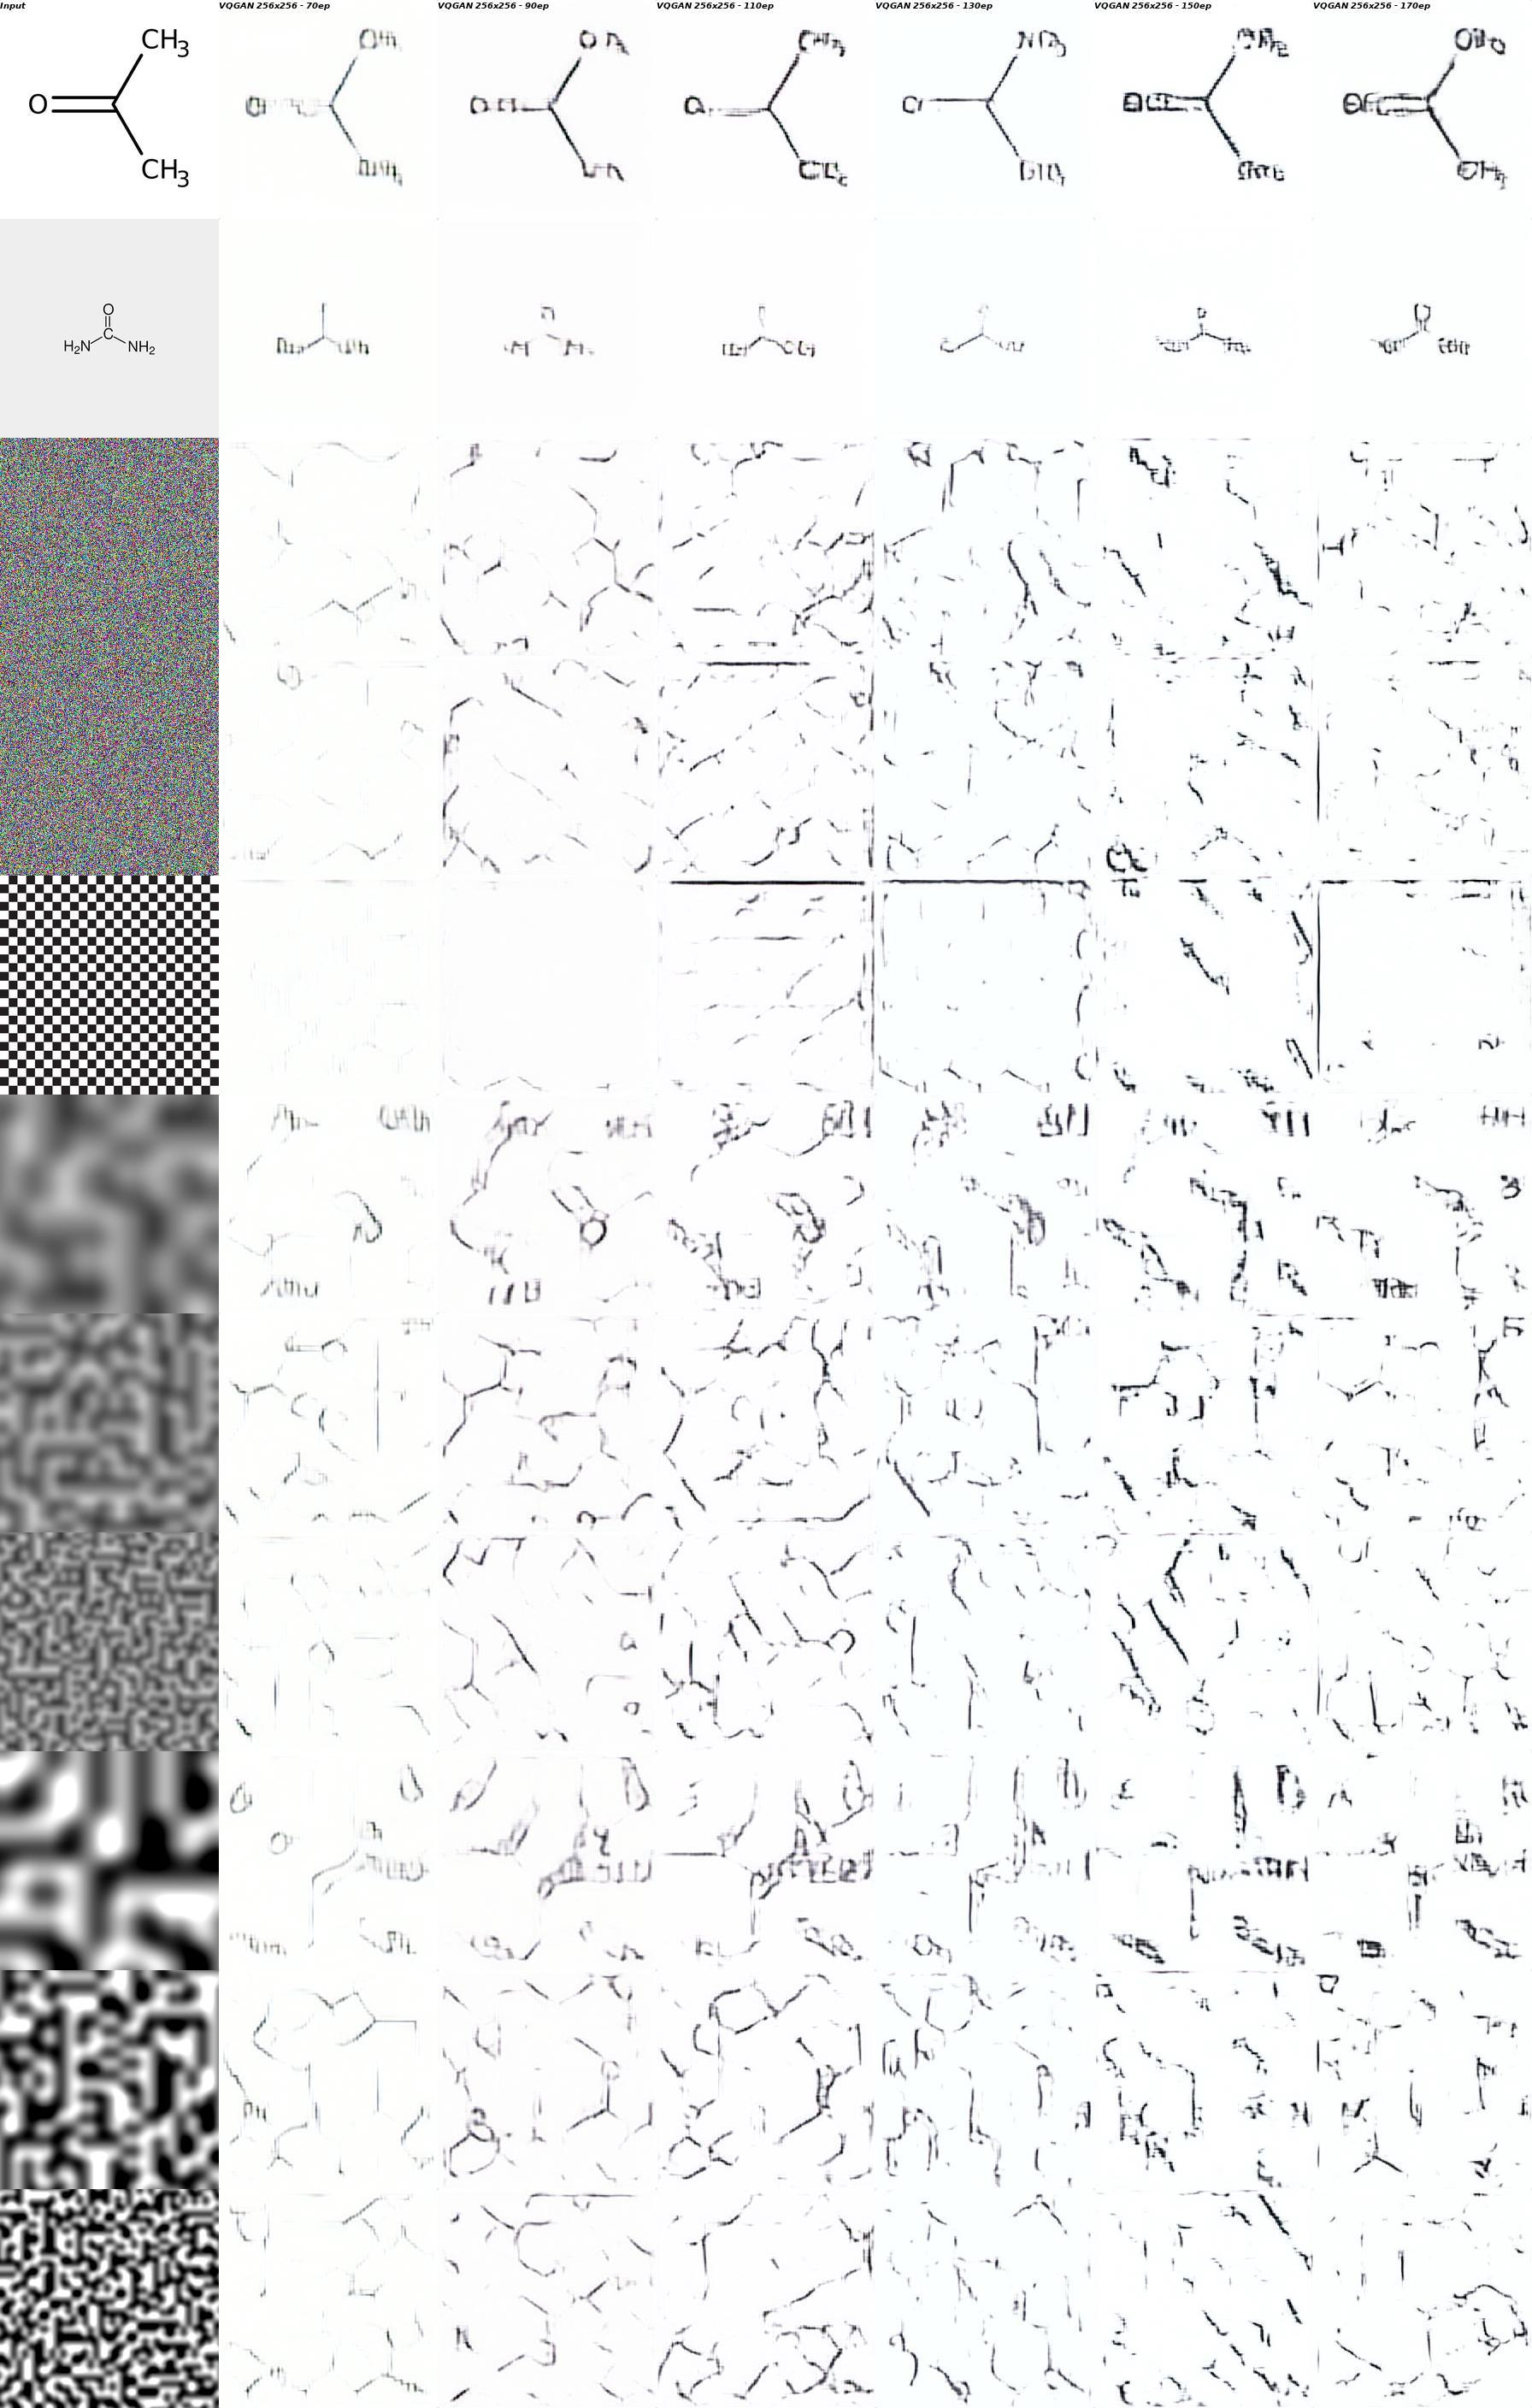
\includegraphics[scale=0.2]{imagenes/image_generation/256/256_1.jpg}}  
    \label{fig:synthetic_molecules}
\end{figure}

\begin{figure}[H]
\centering
    \fbox{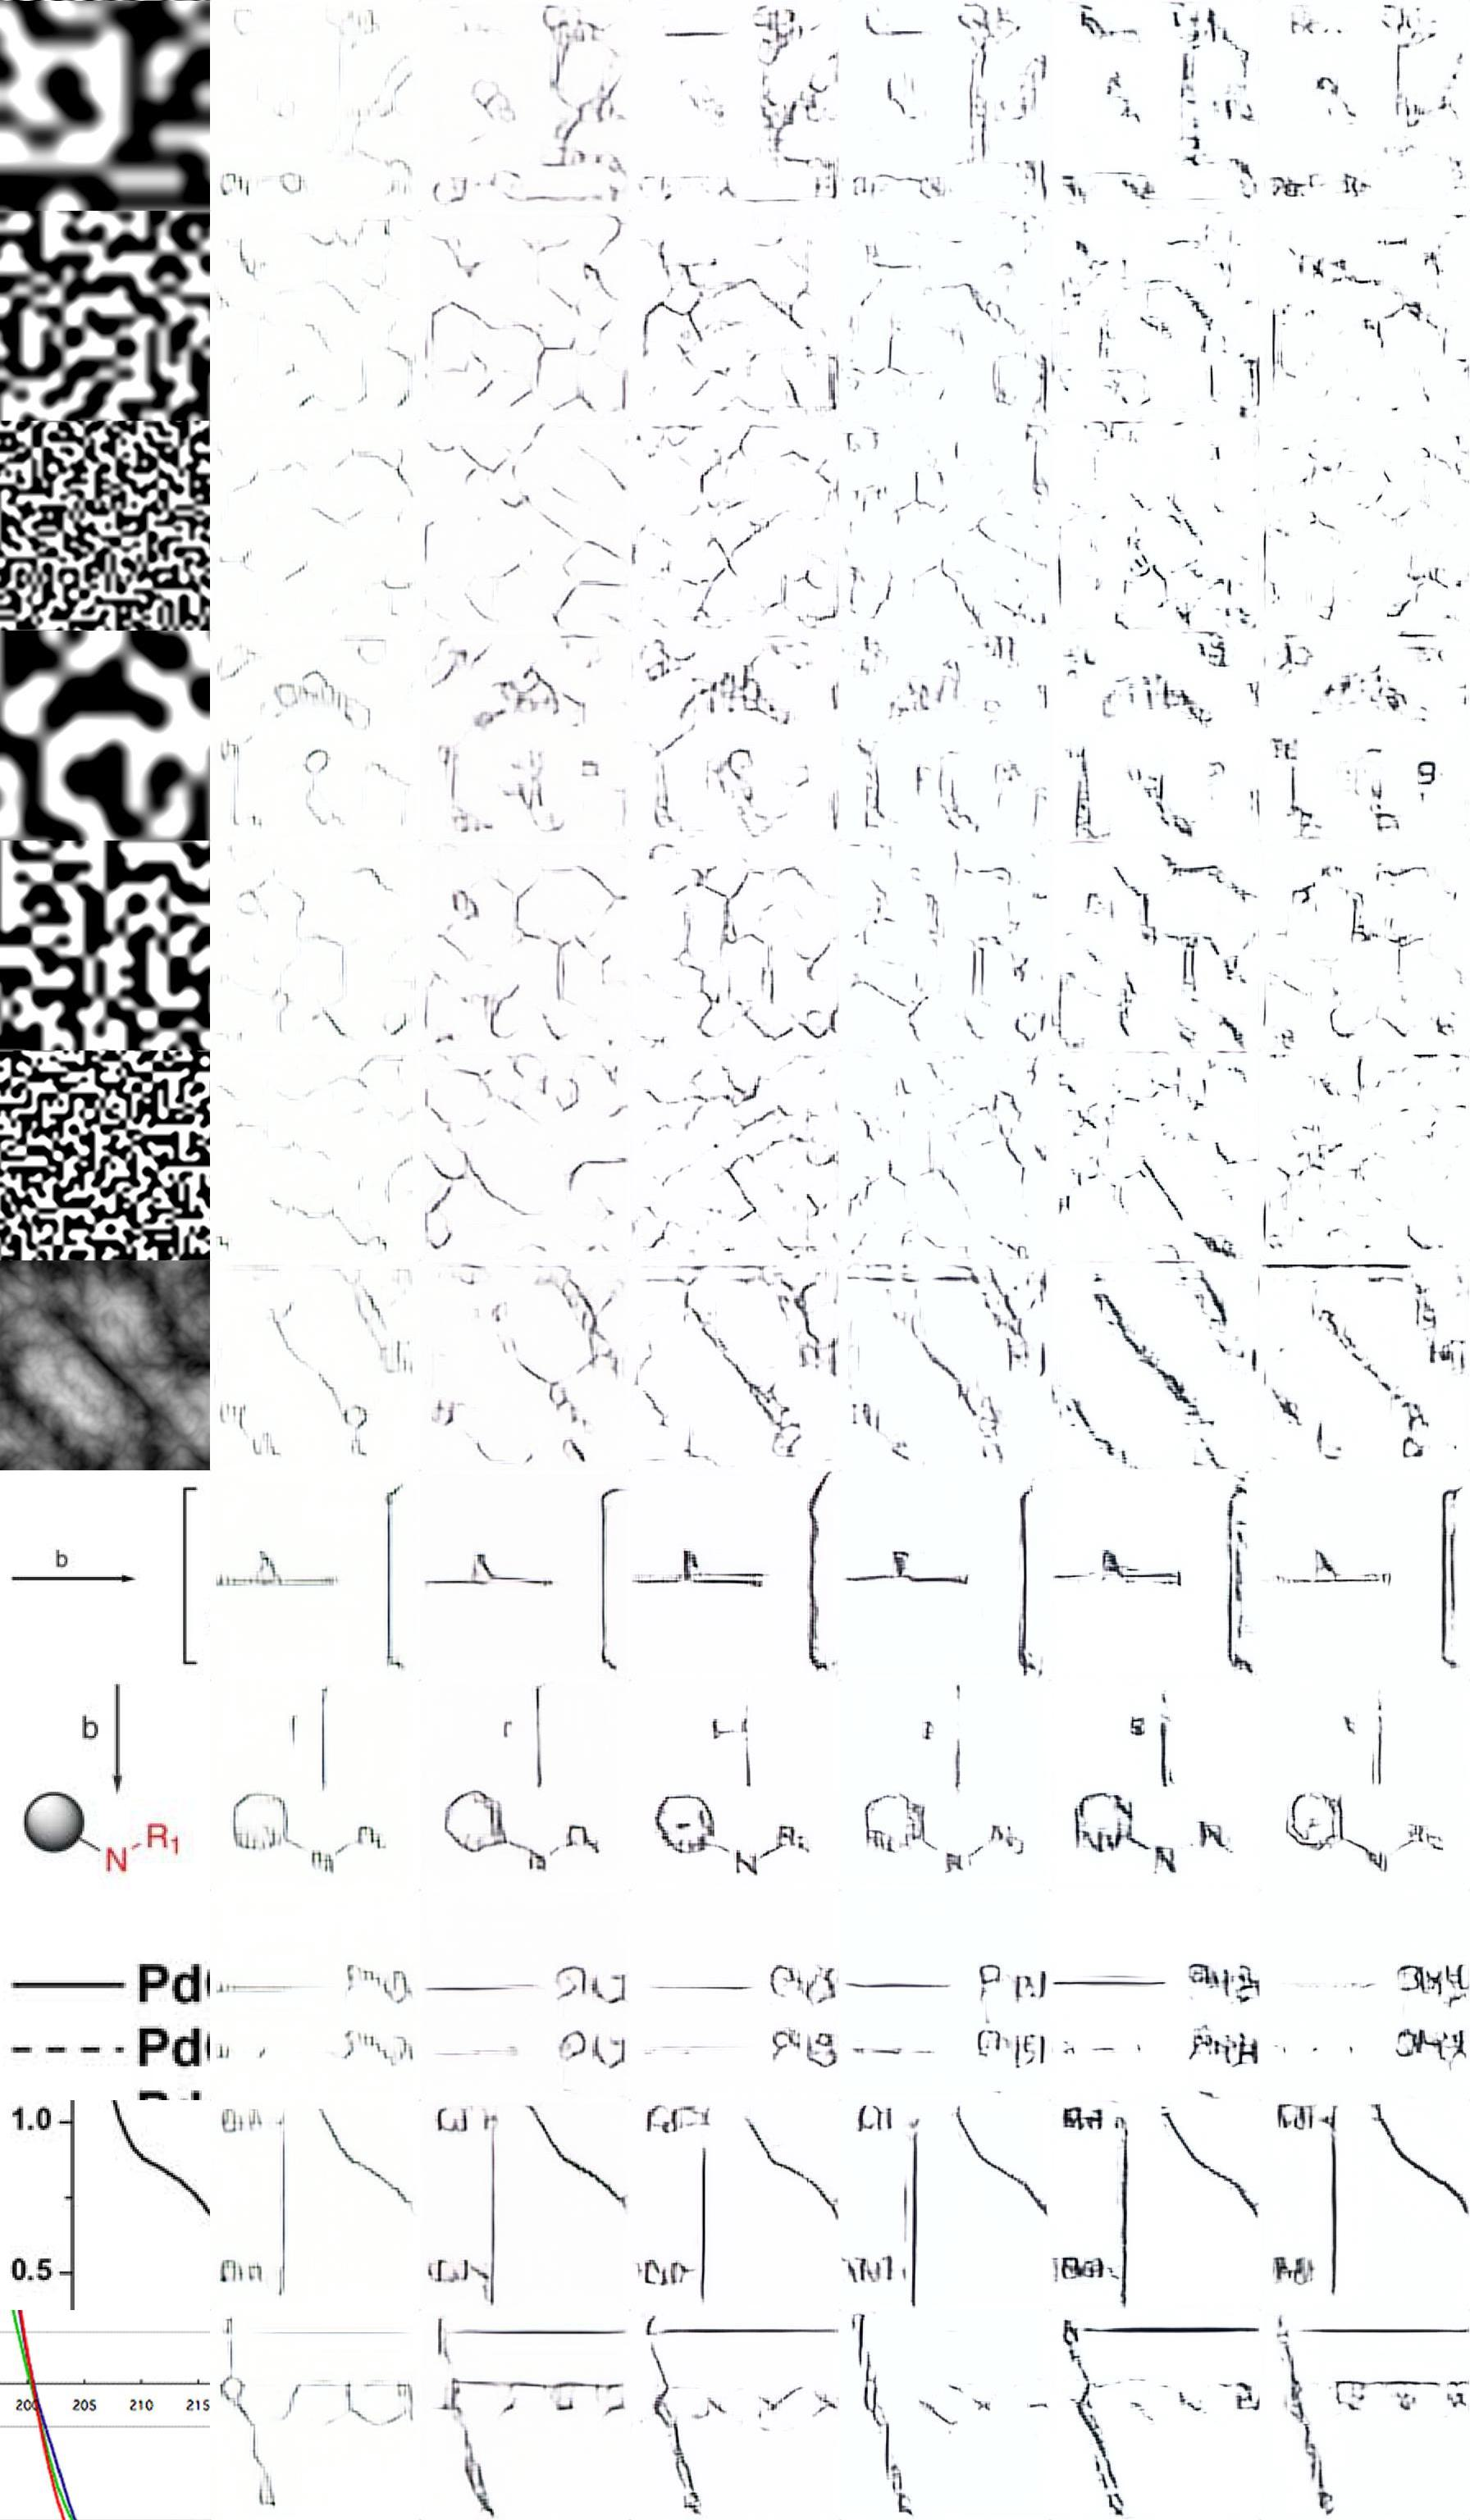
\includegraphics[scale=0.2]{imagenes/image_generation/256/256_2.jpg}}  
\end{figure}


\begin{figure}[H]
\centering
    \caption{Resultados de entrenar los modelos sobre el conjunto de datos con \textit{data augmentation} 1. La primera columna representa la imagen de entrada, el resto los diferentes modelos entrenados desde 70 hasta 170 épocas, tomadas de 20 en 20.} 
    \fbox{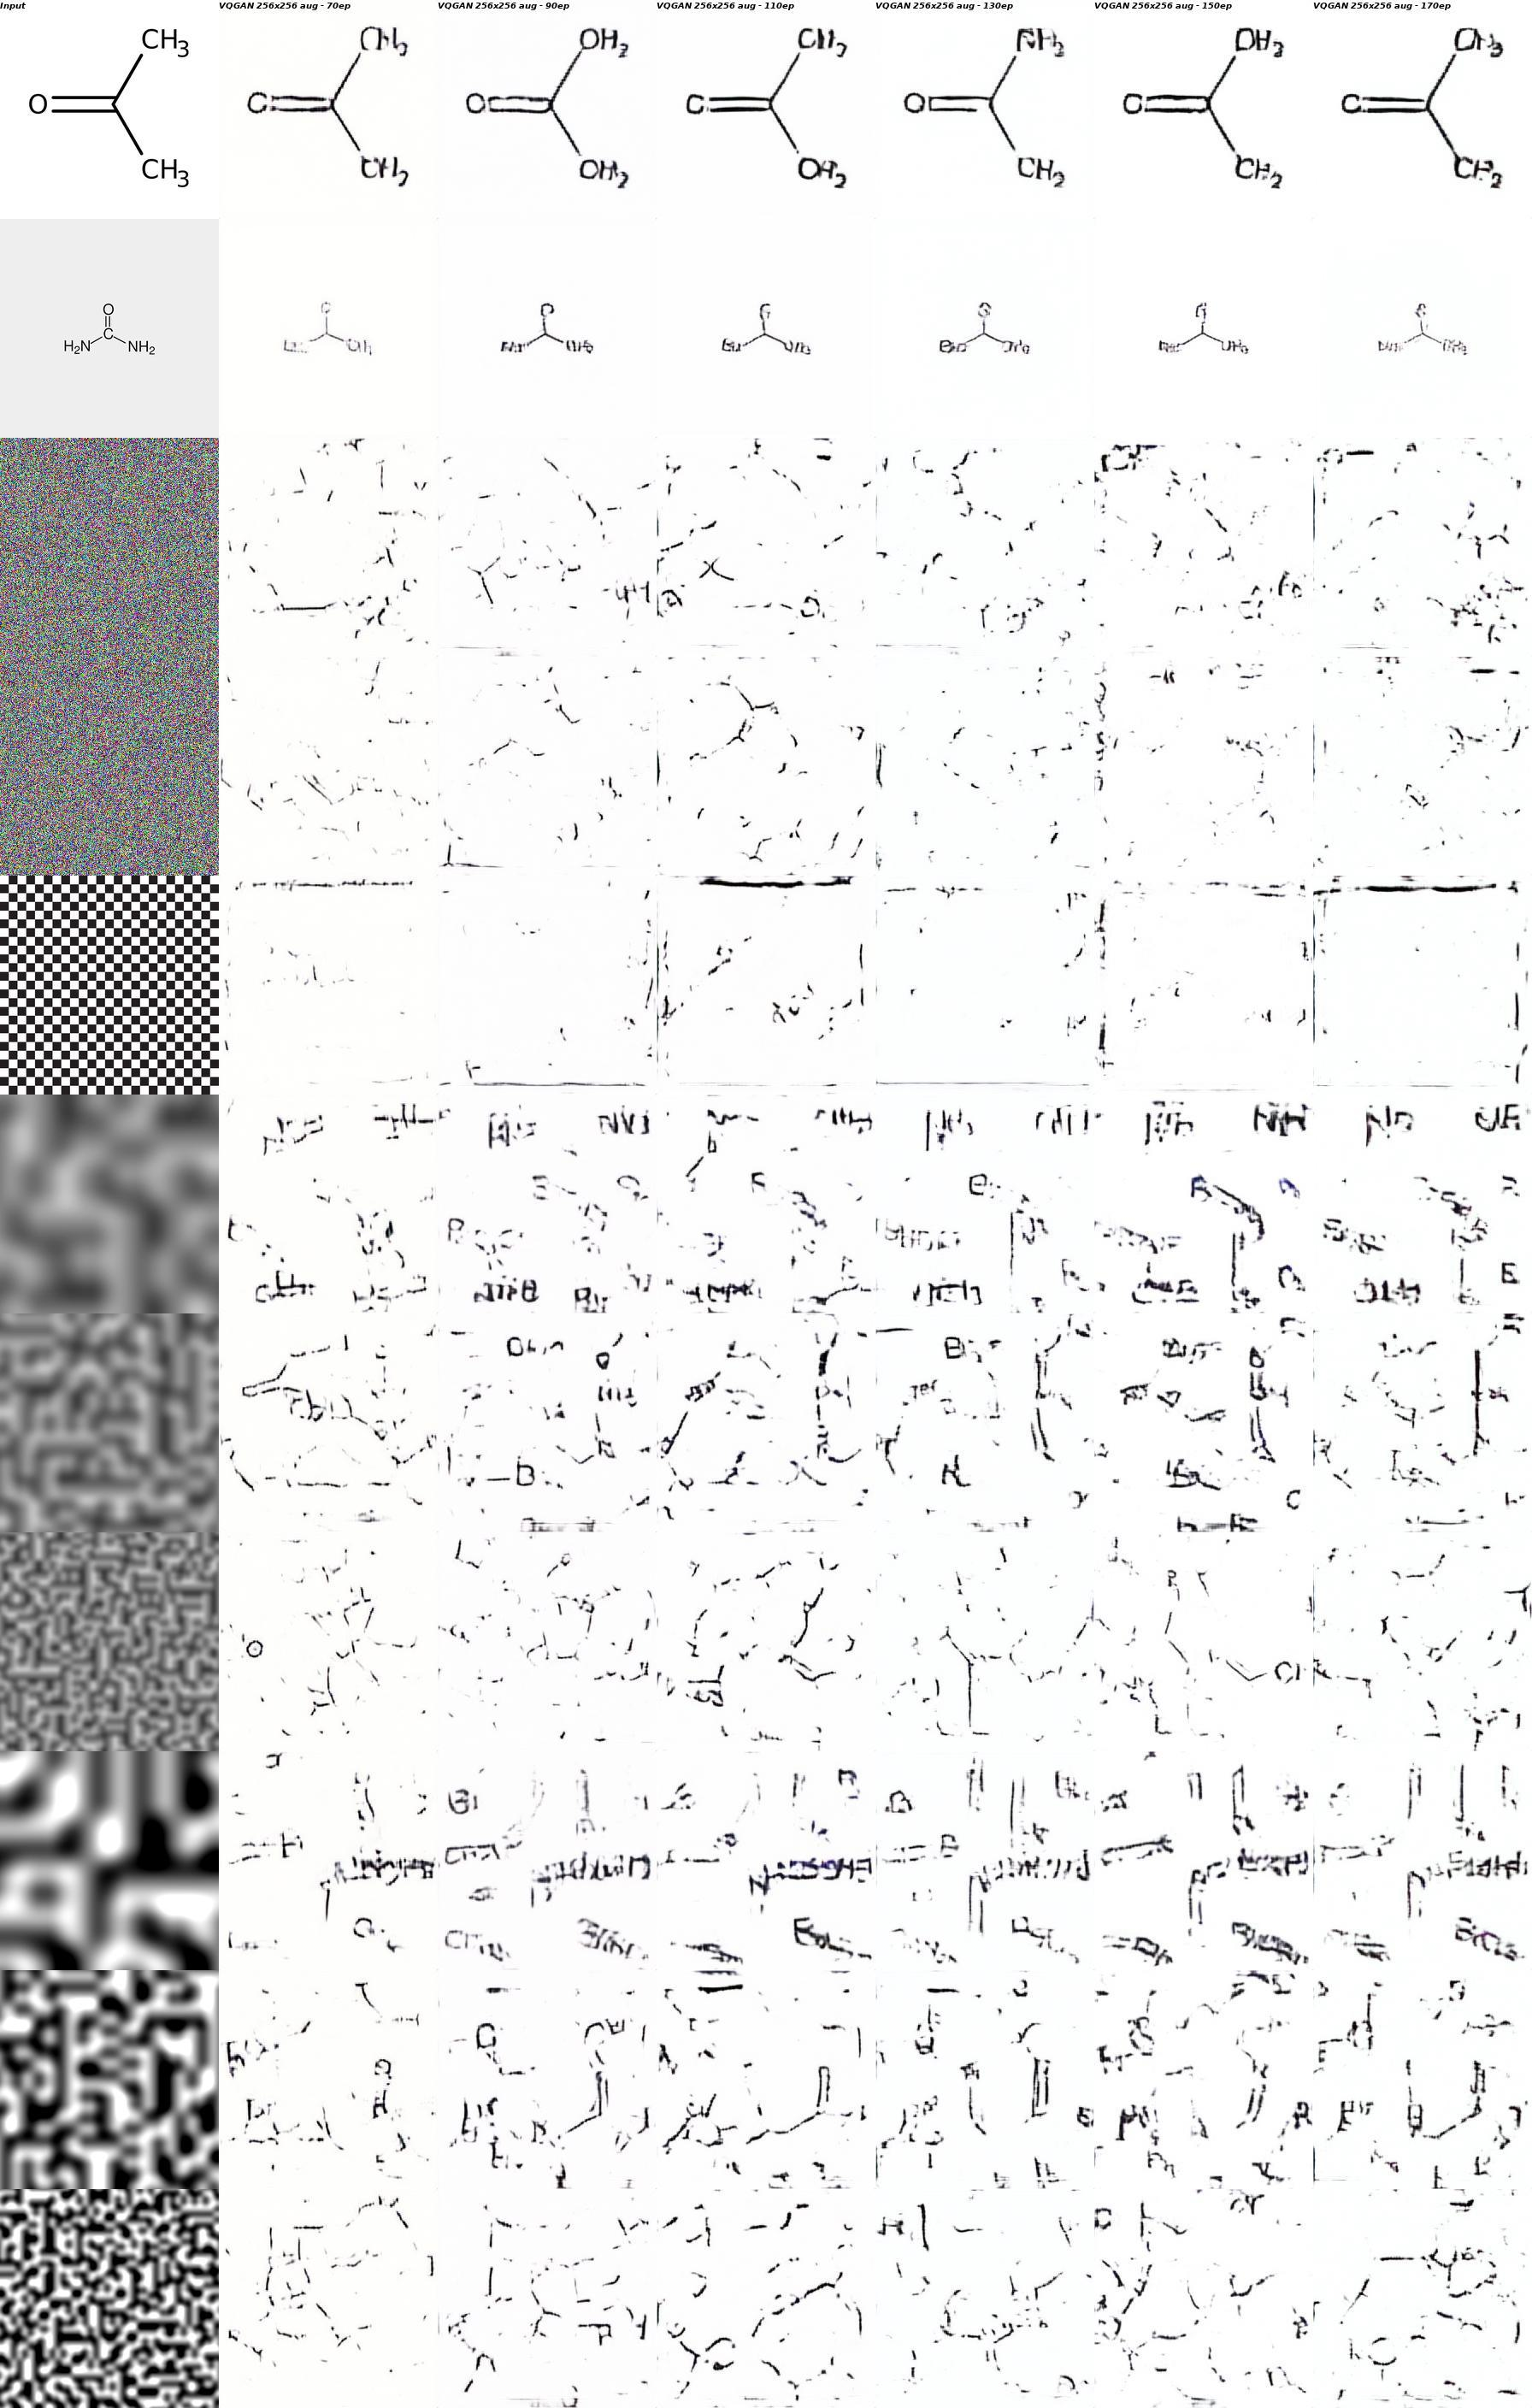
\includegraphics[scale=0.2]{imagenes/image_generation/256/aug_1.jpg}}  
    \label{fig:synthetic_molecules_aug1}
\end{figure}

\begin{figure}[H]
\centering
    \fbox{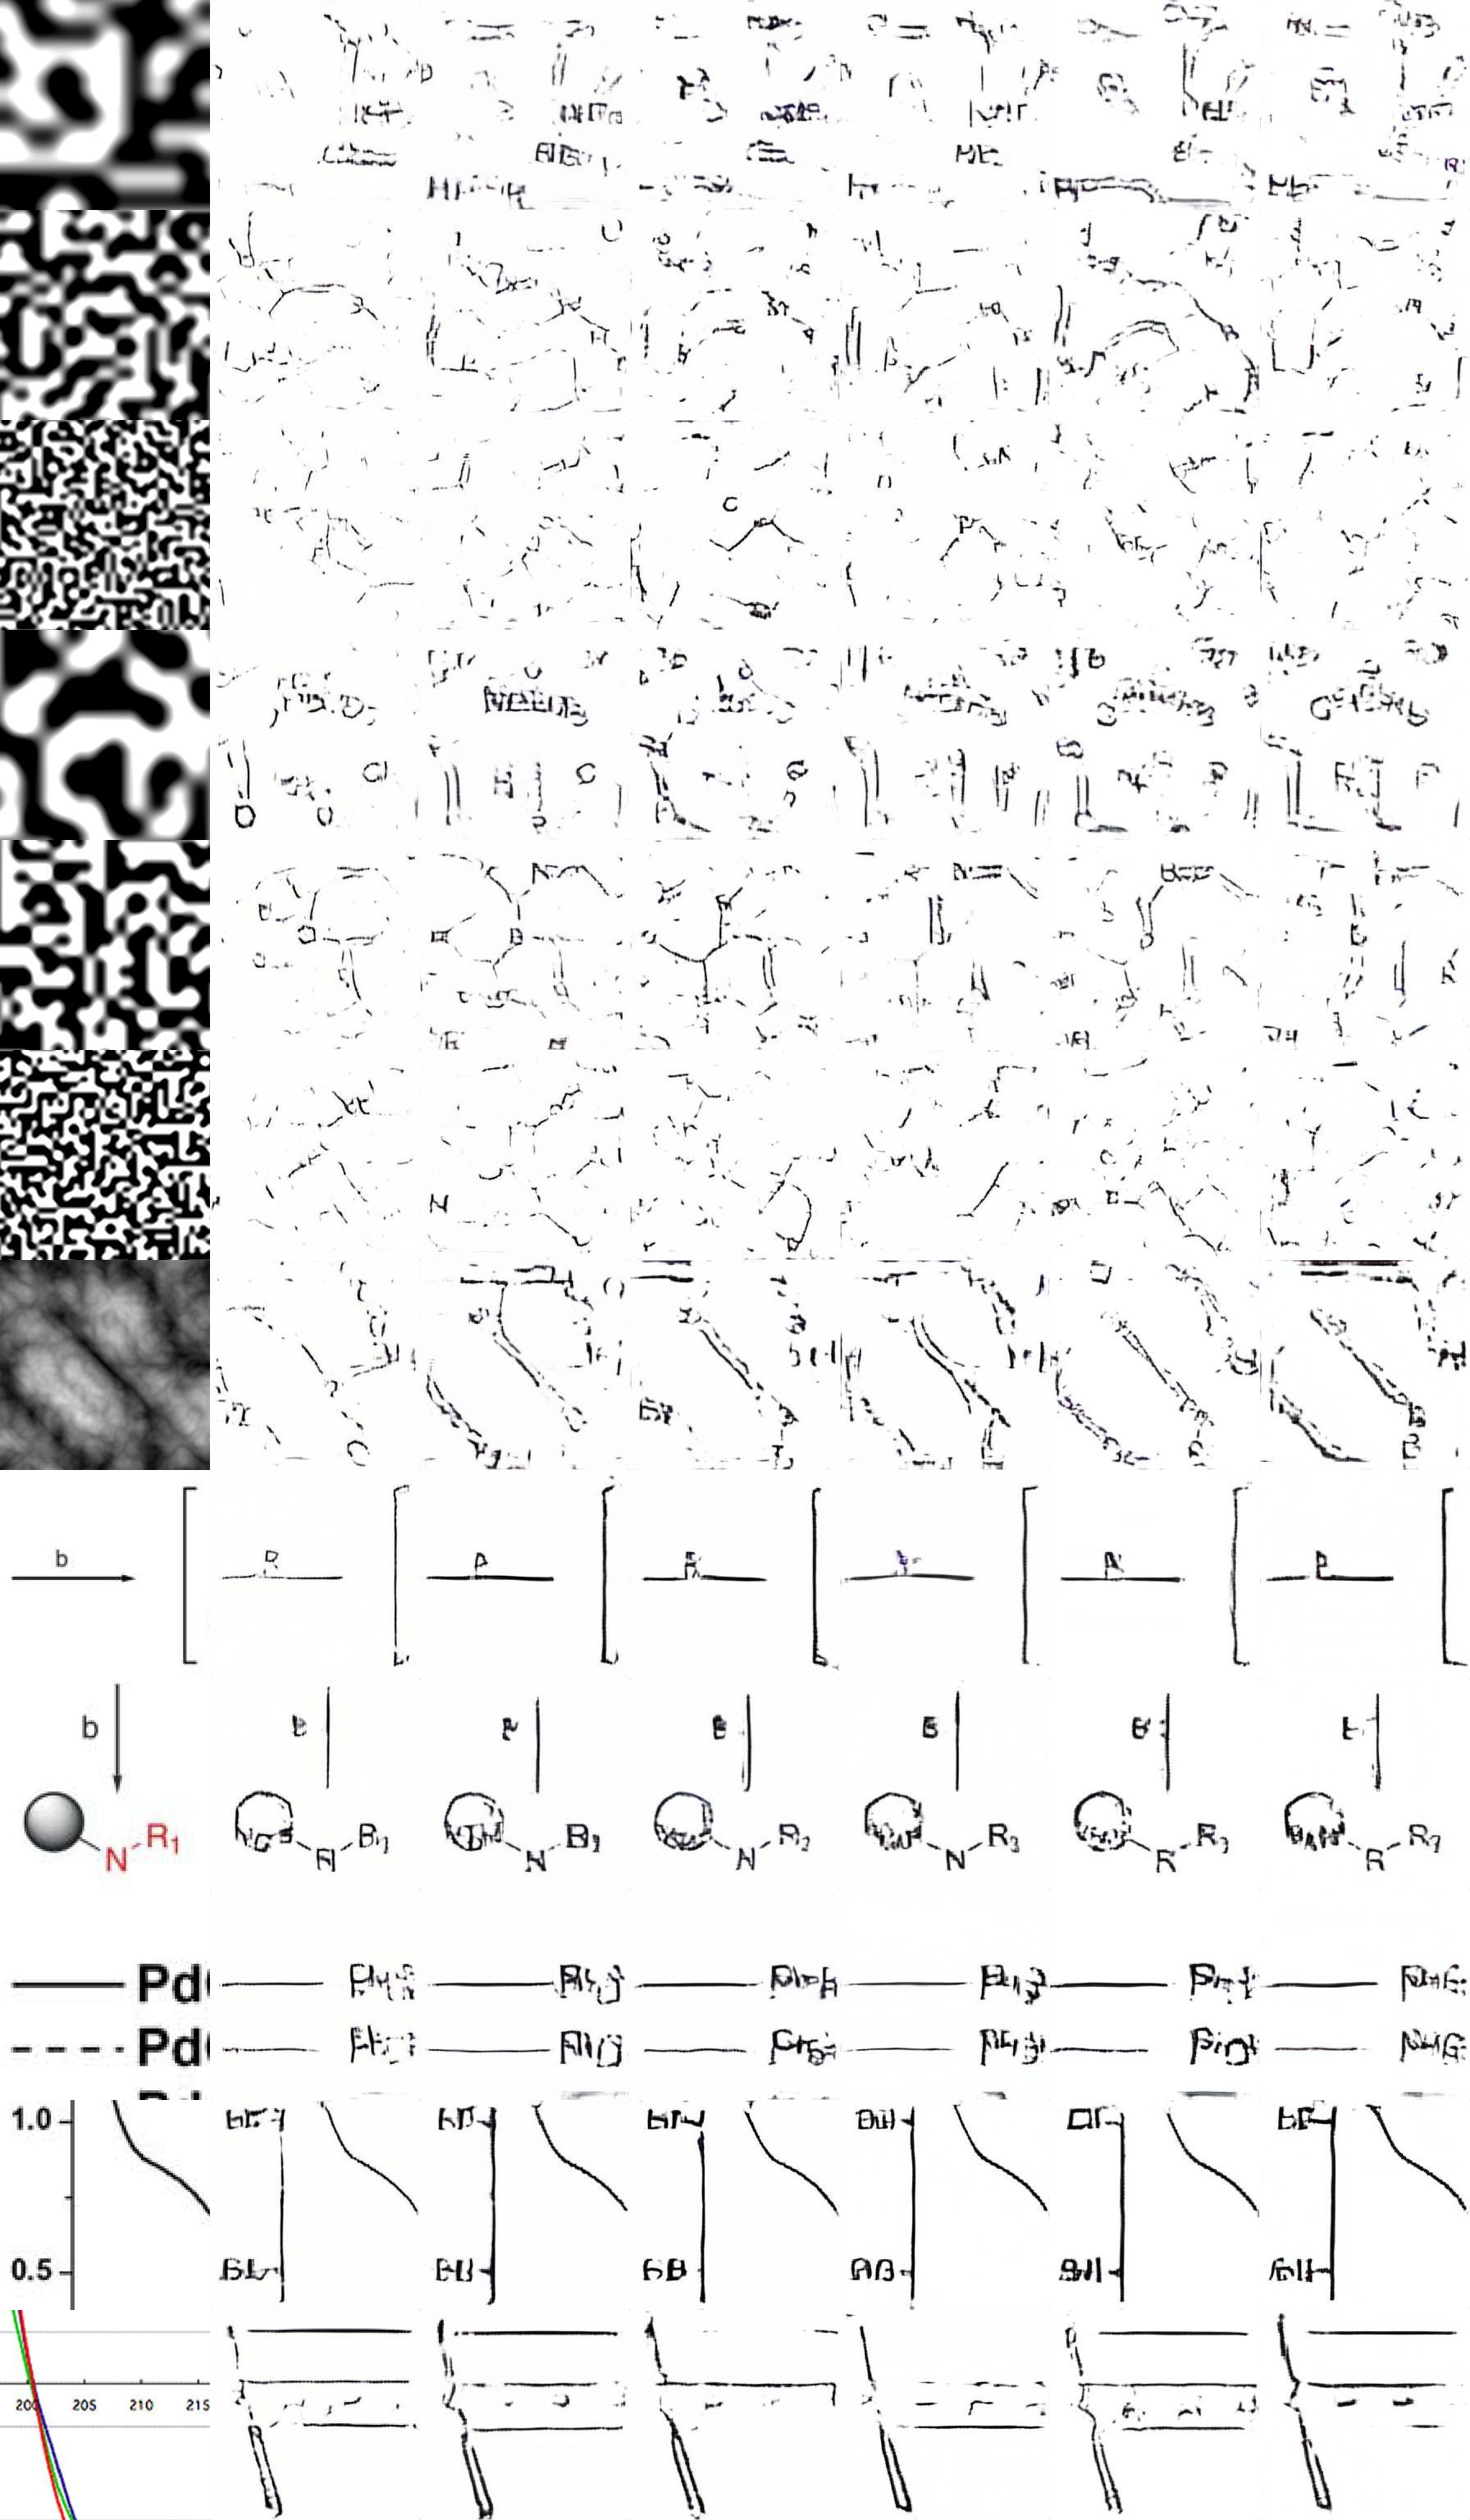
\includegraphics[scale=0.2]{imagenes/image_generation/256/aug_2.jpg}}  
\end{figure}


\begin{figure}[H]
\centering
    \caption{Resultados de entrenar los modelos sobre el conjunto de datos con \textit{data augmentation} 2. La primera columna representa la imagen de entrada, el resto los diferentes modelos entrenados desde 70 hasta 170 épocas, tomadas de 20 en 20.} 
    \fbox{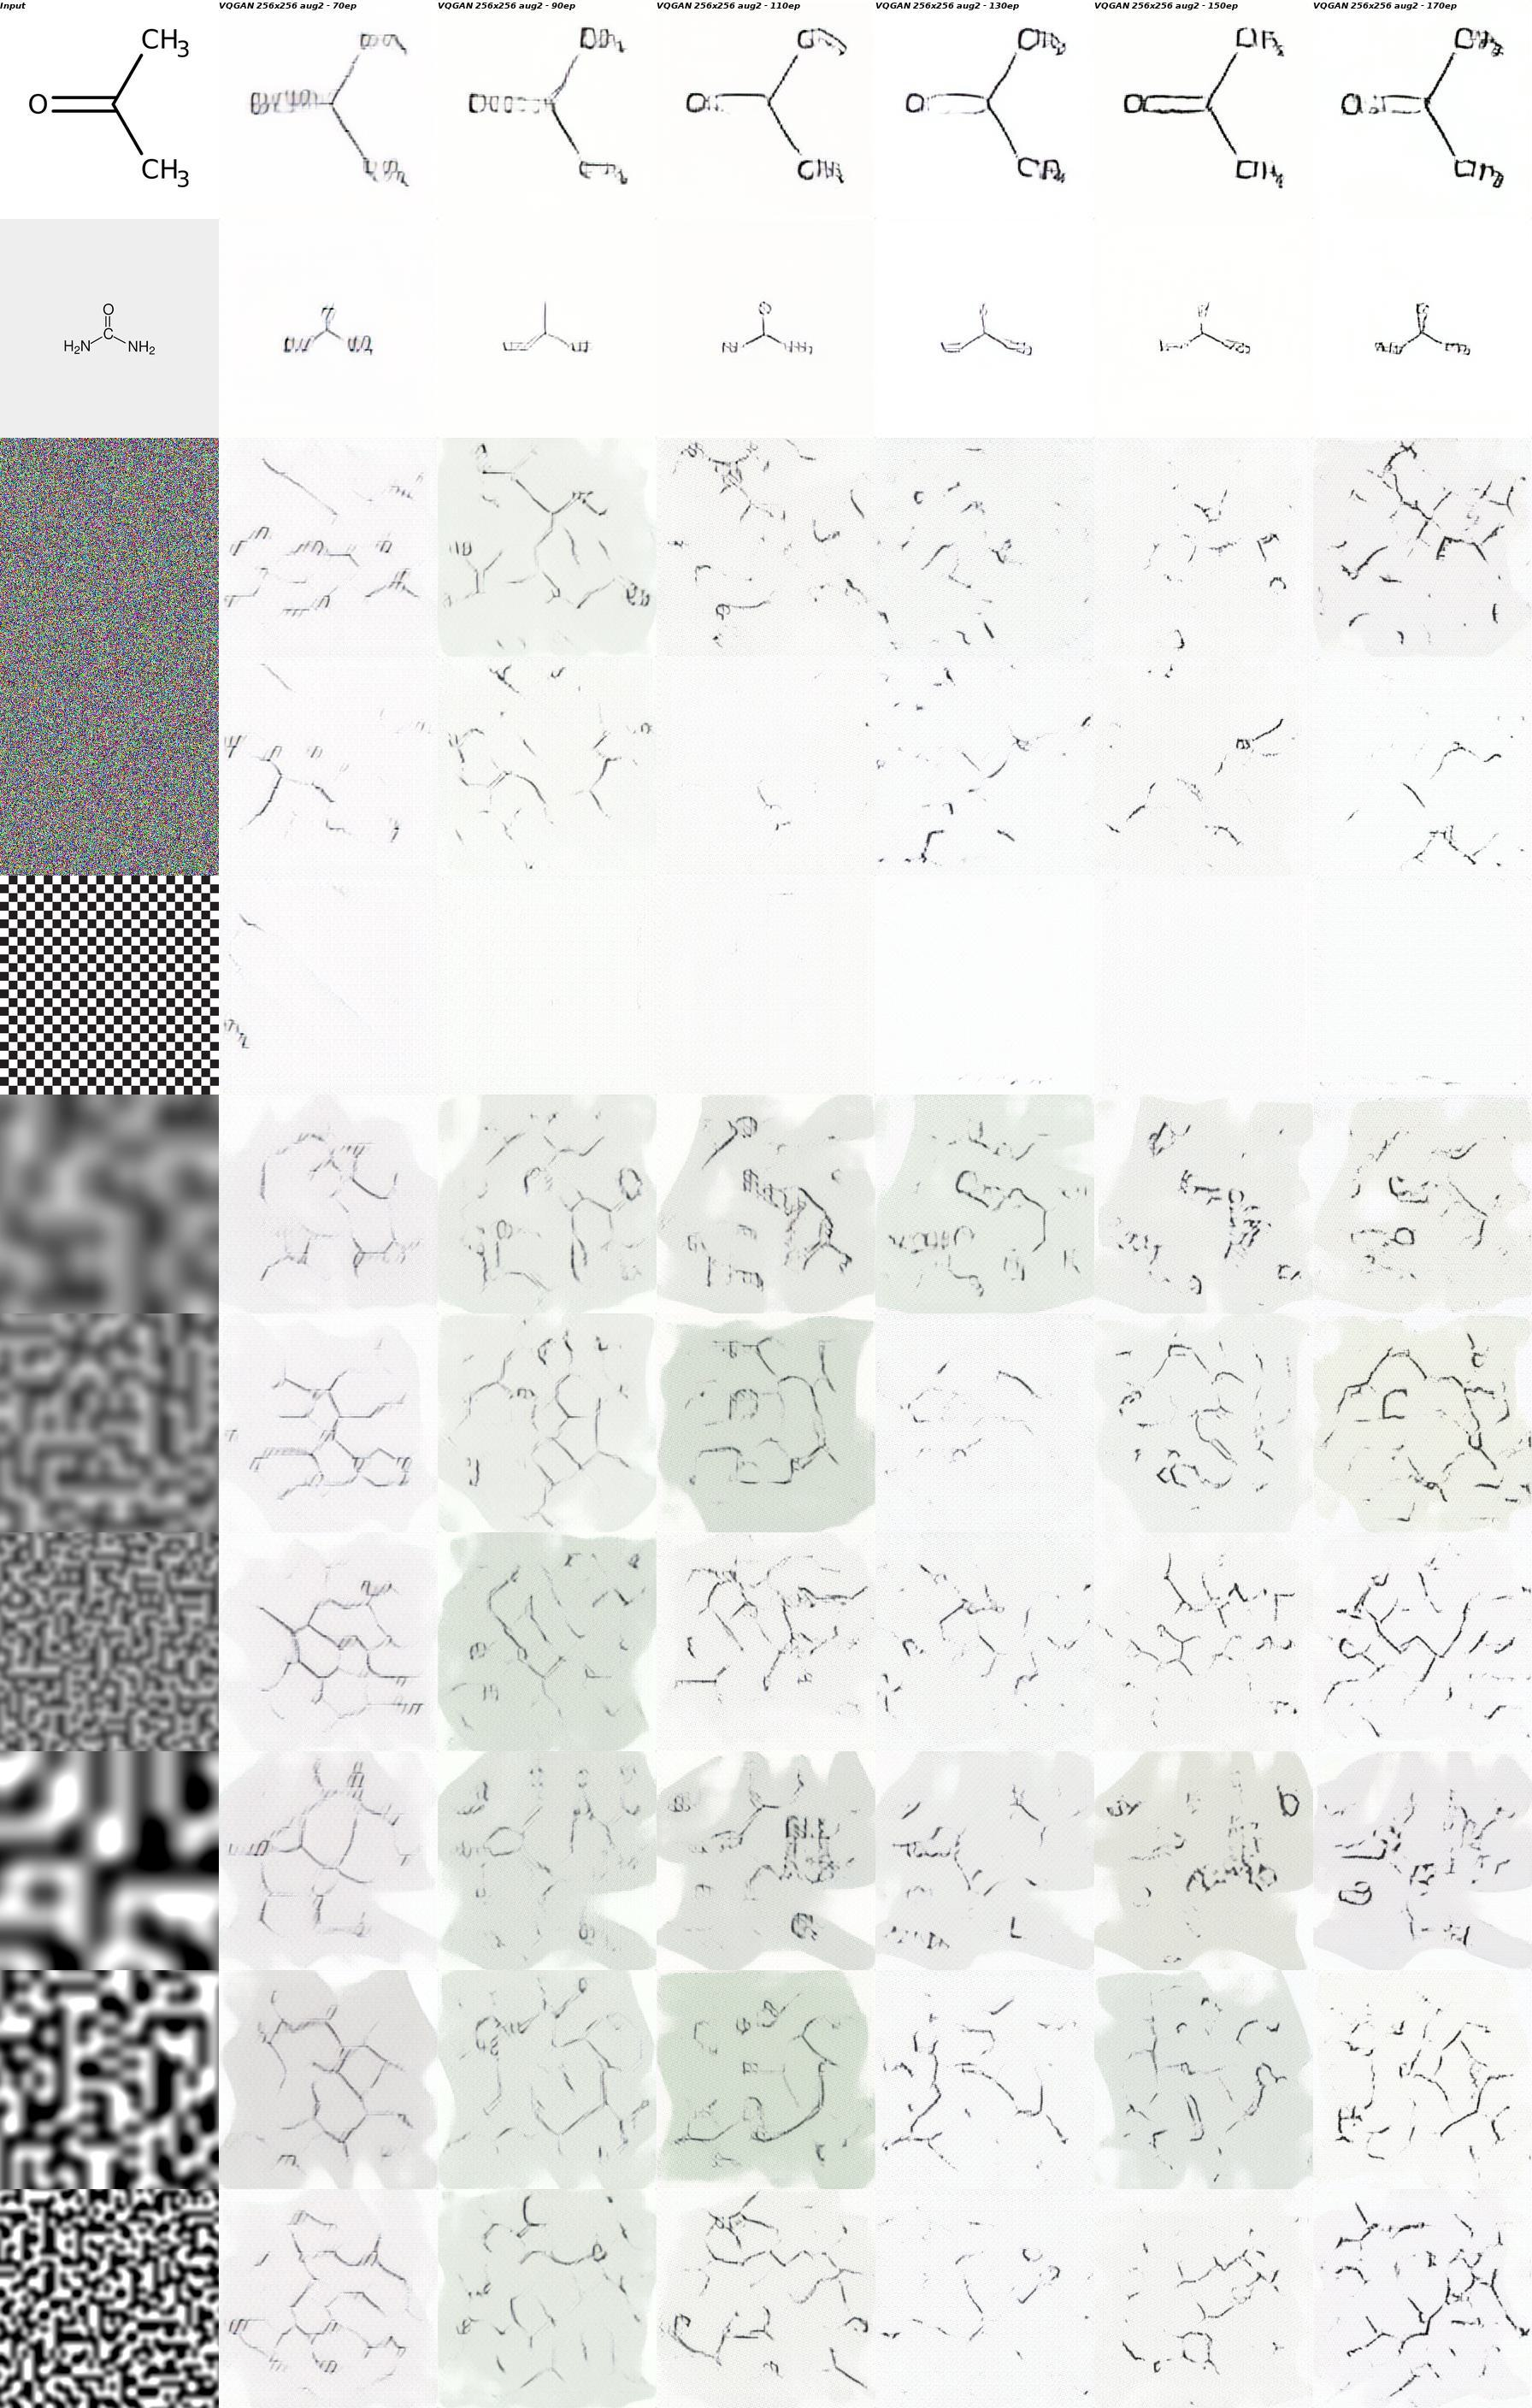
\includegraphics[scale=0.2]{imagenes/image_generation/256/aug2_1.jpg}} 
    \label{fig:synthetic_molecules_aug2} 
\end{figure}

\begin{figure}[H]
\centering
    \fbox{\includegraphics[scale=0.2]{imagenes/image_generation/256/aug2_2.jpg}}  

\end{figure}


\begin{figure}[H]
\centering
    \caption{Resultados de entrenar los modelos sobre el conjunto de datos con \textit{data augmentation} 3. La primera columna representa la imagen de entrada, el resto los diferentes modelos entrenados desde 70 hasta 170 épocas, tomadas de 20 en 20.}
    \fbox{\includegraphics[scale=0.2]{imagenes/image_generation/256/aug3_1.jpg}}  
    \label{fig:synthetic_molecules_aug3}
\end{figure}

\begin{figure}[H]
\centering
    \fbox{\includegraphics[scale=0.2]{imagenes/image_generation/256/aug3_2.jpg}}  
\end{figure}

¿Qué tipo de datos de entrada se han utilizado para generar las imágenes sintéticas? En un primer momento se ha probado a utilizar imágenes de moléculas reales y de objetos que, sin ser moléculas, lo parecen. En el primer caso, la salida es similar a la entrada, con la diferencia de que la imagen sintética pierde información: detalles como letras o números se alteran. En el segundo caso ocurre algo similar, con la particularidad de que objetos circulares son transformados en formas que parecen hexágonos propios de las moléculas. Además, incluso se añaden átomos (Figura \ref{fig:circle-hex}).

\begin{figure}[H]
\centering
    \fbox{\includegraphics[scale=0.3]{imagenes/image_generation/256/circle_to_hex.jpg}}
    \caption{El modelo tiene la capacidad de modificar la imagen para que se parezca a una molécula.}
    \label{fig:circle-hex}
\end{figure}

Pero se quiere poder generar tantas imágenes como sean necesarias, así que se debería poder partir de una imagen de entrada generada aleatoriamente. En un primer momento se utilizó ruido uniforme, pero no funcionó bien en ningún caso. Este tipo de ruido no sigue ninguna estructura, y nuestro modelo necesita una entrada que tenga cierta continuidad. Por ello pruebo con una cuadrícula de ajedrez: ocurre lo mismo, ya que aunque existe un patrón que se repite, los elementos de este no están conectados entre sí.

\subsection{Ruido Perlín}
Se trata de un ruido inventado por Ken Perlín en 1982 que revolucionó el ámbito de la Informática Gráfica. En esta rama de las Ciencias de la Computación, la creación de texturas que imitan materiales de la naturaleza como la madera o el mármol es una tarea importante. Generar estas texturas de una forma manual o mediante un escáner no es una opción escalable.

Este ruido permite simular fenómenos que requieran aleatoriedad a la vez que continuidad. Para ello, genera una serie de gradientes en un \textit{grid} (en nuestro caso 2D). A continuación, interpola el valor de esos gradientes mediante interpolación polinómica de Hermite (Figura \ref{fig:interpolacion}). La ventaja de este ruido frente a otros que también se generan mediante interpolación es su eficiencia, para calcular la interpolación en un punto solo intervienen los $2^n$ gradientes más cercanos, donde $n$ es el número de dimensiones. \cite{computer-graphics-epfl}

\begin{figure}[H]
\centering
    \fbox{\includegraphics[scale=0.3]{imagenes/image_generation/perlin_interpolation.png}}
    \caption{Interpolación de gradientes en el Ruido Perlín 1D. \cite{computer-graphics-epfl}}
    \label{fig:interpolacion}
\end{figure}

El Ruido Perlín se puede modificar cambiando la amplitud y frecuencia de este. A mayor amplitud, los cambios entre zonas del ruido serán más bruscos, a menor amplitud el ruido será más homogéneo y suave. La frecuencia cambia la granularidad del ruido, a mayor frecuencia encontramos un grano más fino. 

\begin{figure}[H]
\centering
    \begin{subfigure}{.26\textwidth}
        \centering
        \includegraphics[width=1\linewidth]{imagenes/image_generation/perlin_python_3_1.jpg}
        \caption{Amp:3 Frec:1}
    \end{subfigure}%
    \begin{subfigure}{.26\textwidth}
        \centering
        \includegraphics[width=1\linewidth]{imagenes/image_generation/perlin_python_3_4.jpg}
        \caption{Amp:3 Frec:4}
    \end{subfigure}%

    \bigskip

    \begin{subfigure}{.26\textwidth}
        \centering
        \includegraphics[width=1\linewidth]{imagenes/image_generation/perlin_python_7_1.jpg}
        \caption{Amp:7 Frec:1}
    \end{subfigure}%
    \begin{subfigure}{.26\textwidth}
        \centering
        \includegraphics[width=1\linewidth]{imagenes/image_generation/perlin_python_7_4.jpg}
        \caption{Amp:7 Frec:4}
    \end{subfigure}

    \caption{Ejemplos de Ruido Perlín con distinta amplitud y frecuencia.}
\end{figure}

Como se observa en las figuras \ref{fig:synthetic_molecules}, \ref{fig:synthetic_molecules_aug1}, \ref{fig:synthetic_molecules_aug2} y \ref{fig:synthetic_molecules_aug3}, al contrario que con el ruido uniforme, este tipo de ruido es capaz de generar imágenes que parecen moléculas. Su continuidad permite que el modelo tenga una estructura en la que basarse para realizar la generación. 

Tras realizar estos experimentos, se los mostré al equipo para conocer su opinión: está conforme con la versión \textit{data augmentation} 2 entrenada durante 70 épocas en aquellos casos en los que se utiliza Ruido Perlín como entrada (figural \ref{fig:synthetic_molecules_aug2}, segunda columna). De todas formas, como se obtienen buenos resultados entre 70 y 90 épocas, voy a entrenar con \textit{data augmentation} 2 durante 70, 75, 80, 85 y 90 épocas y a comparar los resultados.

\begin{figure}[H]
\centering
    \caption{Resultados de entrenar con imágenes con \textit{data augmentation} 2. La primera columna representa la imagen de entrada (ruido Perlín en todos los casos), el resto los diferentes modelos entrenados desde las 70 hasta las 90 épocas tomadas de 5 en 5.}
    \fbox{\includegraphics[scale=0.23]{imagenes/image_generation/256/aug2_extraepochs_1.jpg}}  
    \label{fig:synthetic_molecules_aug2_extra} 
\end{figure}

\begin{figure}[H]
\centering
    \fbox{\includegraphics[scale=0.23]{imagenes/image_generation/256/aug2_extraepochs_2.jpg}}  
\end{figure}

En diferente número de épocas/tipos de ruido Perlín se obtienen buenos resultados, por lo que no voy a utilizar una única configuración para generar los \textit{hard negatives}, se utilizarán varias hasta alcanzar los 400 que quiero generar. 

En concreto, voy a obtener 50 imágenes a partir de cada una de estas configuraciones (todas ellas obtenidas tras entrenar sobre \textit{data augmentation} 2):

\begin{itemize}
    \item Modelo entrenado durante 70 épocas al que se le introduce ruido Perlín con amplitud 1 y frecuencia 2 (fila 2 columna 2 de la figura \ref{fig:synthetic_molecules_aug2_extra}).
    \item Modelo entrenado durante 70 épocas al que se le introduce ruido Perlín con amplitud 1 y frecuencia 4 (fila 3 columna 2 de la figura \ref{fig:synthetic_molecules_aug2_extra}).
    \item Modelo entrenado durante 70 épocas al que se le introduce ruido Perlín con amplitud 3 y frecuencia 2 (fila 5 columna 2 de la figura \ref{fig:synthetic_molecules_aug2_extra}).
    \item Modelo entrenado durante 75 épocas al que se le introduce ruido Perlín con amplitud 1 y frecuencia 4 (fila 3 columna 3 de la figura \ref{fig:synthetic_molecules_aug2_extra}).
    \item Modelo entrenado durante 75 épocas al que se le introduce ruido Perlín con amplitud 3 y frecuencia 2 (fila 5 columna 3 de la figura \ref{fig:synthetic_molecules_aug2_extra}).
    \item Modelo entrenado durante 80 épocas al que se le introduce ruido Perlín con amplitud 1 y frecuencia 2 (fila 2 columna 4 de la figura \ref{fig:synthetic_molecules_aug2_extra}).
    \item Modelo entrenado durante 85 épocas al que se le introduce ruido Perlín con amplitud 1 y frecuencia 2 (fila 2 columna 5 de la figura \ref{fig:synthetic_molecules_aug2_extra}).
    \item Modelo entrenado durante 85 épocas al que se le introduce ruido Perlín con amplitud 7 y frecuencia 2 (fila 11 columna 5 de la figura \ref{fig:synthetic_molecules_aug2_extra}).
\end{itemize}

En total, 400 \textit{hard negatives}. Antes de unificarlos con 400 ejemplos negativos del \textit{dataset} original, los trato de forma que se reduce el color grisáceo de fondo que presentan tras ser producidos por los modelos generadores. Para ello, de forma independiente en cada una de las configuraciones, fijo un umbral de color que, si no es superado por un pixel, este es transformado en color blanco. De esta forma, solo los píxeles con un color intenso se mantienen en la imagen, o sea, solo se mantiene la estructura molecular. Antes de eso, aplico un aumento de contraste a la imagen y un filtro de apertura (\textit{opening}) que elimina ruido. Algunos ejemplos resultantes se pueden observar en la Figura \ref{fig:hard-negatives}.

\begin{figure}[H]
\centering
    \begin{subfigure}{.28\textwidth}
        \centering
        \includegraphics[width=1\linewidth]{imagenes/image_generation/clean_results/perlin_e70_a1_f2_2.jpg}
    \end{subfigure}%
    \begin{subfigure}{.28\textwidth}
        \centering
        \includegraphics[width=1\linewidth]{imagenes/image_generation/clean_results/perlin_e75_a1_f4_33.jpg}
    \end{subfigure}%

    \bigskip

    \begin{subfigure}{.28\textwidth}
        \centering
        \includegraphics[width=1\linewidth]{imagenes/image_generation/clean_results/perlin_e80_a1_f2_13.jpg}
    \end{subfigure}%
    \begin{subfigure}{.28\textwidth}
        \centering
        \includegraphics[width=1\linewidth]{imagenes/image_generation/clean_results/perlin_e85_a7_f2_42.jpg}
    \end{subfigure}

    \caption{\textit{Hard negatives} finales tras ser post-procesados.}
    \label{fig:hard-negatives}
\end{figure}

Ya puedo crear los dos \textit{datasets} finales para entrenar el clasificador, tal y como se expone en la Figura \ref{fig:two_final_datasets} del capítulo anterior.

\newpage
Otra prueba que se hizo y fue descartada consistió en entrenar el modelo generador a partir de ejemplos negativos. Si, en vez de entrenar sobre ejemplos positivos como estaba haciendo hasta ahora, hacerlo sobre negativos. ¿Qué ocurrió? Como se puede observar en la Figura \ref{fig:extraepochs}, los resultados no fueron buenos.

\begin{figure}[H]
\centering
    \caption{Resultados de entrenar con ejemplos negativos. La primera columna representa la imagen de entrada, el resto los diferentes modelos entrenados desde las 70 hasta las 170 épocas tomadas de 20 en 20.}
    \fbox{\includegraphics[scale=0.2]{imagenes/image_generation/negative256/negative256.jpg}}
    \label{fig:extraepochs}
\end{figure}

Esto puede deberse a la alta diversidad que presentan los ejemplos negativos del \textit{dataset}. Esta diversidad hace que el modelo generativo no pueda aprender, ya que las imágenes no tienen apenas características en común.

Por tanto, existen dos datasets finales con los que se entrenará cada una de las versiones del clasificador (Ver Figura \ref{fig:two_final_datasets}).
\begin{figure}[H]
\centering
    \fbox{\includegraphics[scale=0.42]{imagenes/metodologia/two_datasets_aug2.png}}  
    \caption{Dos \textit{datasets} para entrenar dos clasificadores.} 
    \label{fig:two_final_datasets}
\end{figure}

\newpage
\section{Clasificación de imágenes}

Con los dos \textit{datasets} preparados \ref{fig:two_final_datasets}, paso a construir los clasificadores. Como se mencionó en el capítulo anterior, llevaré a cabo una \textit{grid search} para comprobar que arquitecturas e hiperparámetros funcionan mejor.

El código en el que se realizan los experimentos con el clasificador se encuentra principalmente en los siguientes archivos:

\vspace{0.2cm}
\dirtree{%
    .1 experiments/\DTcomment{implementación del TFG}.
    .2 image\_classifier/\DTcomment{clasificador de imágenes}.
    .3 datasets.py.
    .3 models.py.
    .3 grid\_search.py.
    .3 train\_final\_models.py.
    .3 train\_lenet.py
    .3 functions.py.
}

\noindent \textit{datasets.py} declara la clase CompoundDataset, una clase que hereda la clase Dataset de Pytorch. Este objeto facilita la carga de las imágenes y su uso por las funciones y sentencias incluidas en PyTorch.

\noindent \textit{models.py} implementa cada una de las arquitecturas con las que voy a trabajar (LeNet5, AlexNet y VGG16). Se declaran cada una de sus capas, funciones de activación y el orden en el que la información fluye por estas.

\noindent \textit{grid\_search.py} implementa la \textit{grid\_search}, mediante un parámetro podemos indicar si queremos realizarla entrenando los modelos sobre el \textit{dataset} con \textit{hard negatives} o sin ellos.

\noindent \textit{train\_final\_models.py} entrena los modelos finales con la configuración decidida tras realizar la \textit{grid\_search.py}.

\noindent \textit{train\_lenet.py} entrena modelos con LeNet5 utilizando diferentes tamaños de dataset, para estudiar como estudia el tamaño de este al decrecimiento del error de entrenamiento.

\noindent \textit{functions.py} declara funciones utilizadas por todos estos ficheros.

\newpage
\subsection{Clasificador sobre el \textit{dataset} sin \textit{hard negatives}}
Tras ejecutar la \textit{grid search}, se obtienen los siguientes resultados:

\begin{table}[H]
    \footnotesize
    \caption{\textit{Grid search} utilizando la arquitectura LeNet5, entrenamiento sobre \textit{dataset} sin \textit{hard negatives}.}
    \label{table:lenet-sin-hard}
\begin{tabular}{cl|llllll|}
\cline{3-8}
\multicolumn{2}{c|}{\multirow{2}{*}{}} &
    \multicolumn{6}{c|}{Optimizadores} \\ \cline{3-8} 
\multicolumn{2}{c|}{} &
    \multicolumn{2}{c|}{SGD} &
    \multicolumn{2}{c|}{Adam} &
    \multicolumn{2}{c|}{Adadelta} \\ \hline
\multicolumn{1}{|c|}{\begin{tabular}[c]{@{}c@{}}Ini. de \\ pesos\end{tabular}} &
    \multicolumn{1}{c|}{\begin{tabular}[c]{@{}c@{}}Tasa de \\ aprendizaje\end{tabular}} &
    \multicolumn{1}{c}{\begin{tabular}[c]{@{}c@{}}Error\\ medio\\ (\%)\end{tabular}} &
    \multicolumn{1}{c|}{\begin{tabular}[c]{@{}c@{}}Desv.\\ típica\\ (\%)\end{tabular}} &
    \multicolumn{1}{c}{\begin{tabular}[c]{@{}c@{}}Error\\ medio\\ (\%)\end{tabular}} &
    \multicolumn{1}{c|}{\begin{tabular}[c]{@{}c@{}}Desv.\\ típica\\ (\%)\end{tabular}} &
    \multicolumn{1}{c}{\begin{tabular}[c]{@{}c@{}}Error\\ medio\\ (\%)\end{tabular}} &
    \multicolumn{1}{c|}{\begin{tabular}[c]{@{}c@{}}Desv.\\ típica\\ (\%)\end{tabular}} \\ \hline
\multicolumn{1}{|c|}{\multirow{7}{*}{He}} &
    0.5 &
    44.715 &
    \multicolumn{1}{l|}{1.971} &
    49.593 &
    \multicolumn{1}{l|}{6.630} &
    44.715 &
    3.042 \\
\multicolumn{1}{|c|}{} &
    0.05 &
    48.130 &
    \multicolumn{1}{l|}{6.308} &
    44.715 &
    \multicolumn{1}{l|}{3.042} &
    44.715 &
    3.042 \\
\multicolumn{1}{|c|}{} &
    0.005 &
    44.715 &
    \multicolumn{1}{l|}{3.042} &
    44.715 &
    \multicolumn{1}{l|}{3.042} &
    44.715 &
    3.042 \\
\multicolumn{1}{|c|}{} &
    0.0005 &
    44.715 &
    \multicolumn{1}{l|}{3.042} &
    44.715 &
    \multicolumn{1}{l|}{3.042} &
    44.715 &
    3.042 \\
\multicolumn{1}{|c|}{} &
    0.00005 &
    44.715 &
    \multicolumn{1}{l|}{3.042} &
    44.715 &
    \multicolumn{1}{r|}{3.042} &
    48.130 &
    6.308 \\
\multicolumn{1}{|c|}{} &
    0.000005 &
    48.130 &
    \multicolumn{1}{l|}{6.308} &
    44.715 &
    \multicolumn{1}{r|}{3.042} &
    48.130 &
    6.308 \\
\multicolumn{1}{|c|}{} &
    0.0000005 &
    48.130 &
    \multicolumn{1}{l|}{6.308} &
    48.130 &
    \multicolumn{1}{r|}{6.308} &
    48.130 &
    6.308 \\ \hline
\multicolumn{1}{|c|}{\multirow{7}{*}{Xavier}} &
    0.5 &
    48.130 &
    \multicolumn{1}{l|}{6.308} &
    48.943 &
    \multicolumn{1}{l|}{6.540} &
    26.260 &
    \multicolumn{1}{r|}{16.213} \\
\multicolumn{1}{|c|}{} &
    0.05 &
    27.967 &
    \multicolumn{1}{l|}{14.734} &
    44.715 &
    \multicolumn{1}{l|}{3.042} &
    33.252 &
    11.226 \\
\multicolumn{1}{|c|}{} &
    0.005 &
    43.902 &
    \multicolumn{1}{l|}{4.378} &
    44.715 &
    \multicolumn{1}{l|}{3.042} &
    43.740 &
    4.685 \\
\multicolumn{1}{|c|}{} &
    0.0005 &
    44.715 &
    \multicolumn{1}{l|}{3.042} &
    44.715 &
    \multicolumn{1}{r|}{3.042} &
    44.715 &
    3.042 \\
\multicolumn{1}{|c|}{} &
    0.00005 &
    44.715 &
    \multicolumn{1}{l|}{3.042} &
    41.951 &
    \multicolumn{1}{r|}{6.018} &
    48.130 &
    6.308 \\
\multicolumn{1}{|c|}{} &
    0.000005 &
    48.130 &
    \multicolumn{1}{l|}{6.308} &
    40.813 &
    \multicolumn{1}{l|}{6.596} &
    48.130 &
    6.308 \\
\multicolumn{1}{|c|}{} &
    0.0000005 &
    48.130 &
    \multicolumn{1}{l|}{6.308} &
    44.715 &
    \multicolumn{1}{l|}{3.042} &
    48.130 &
    6.308 \\ \hline
\end{tabular}
\label{table:lenetsinhard}
\end{table}


% Please add the following required packages to your document preamble:
% \usepackage{multirow}
\begin{table}[H]
    \footnotesize
    \caption{\textit{Grid search} utilizando la arquitectura AlexNet, entrenamiento sobre \textit{dataset} sin \textit{hard negatives}.}
    \label{table:alexnet-sin-hard}
\begin{tabular}{cl|llllll|}
\cline{3-8}
\multicolumn{2}{c|}{\multirow{2}{*}{}} &
    \multicolumn{6}{c|}{Optimizadores} \\ \cline{3-8} 
\multicolumn{2}{c|}{} &
    \multicolumn{2}{c|}{SGD} &
    \multicolumn{2}{c|}{Adam} &
    \multicolumn{2}{c|}{Adadelta} \\ \hline
\multicolumn{1}{|c|}{\begin{tabular}[c]{@{}c@{}}Ini. de \\ pesos\end{tabular}} &
    \multicolumn{1}{c|}{\begin{tabular}[c]{@{}c@{}}Tasa de \\ aprendizaje\end{tabular}} &
    \multicolumn{1}{c}{\begin{tabular}[c]{@{}c@{}}Error\\ medio\\ (\%)\end{tabular}} &
    \multicolumn{1}{c|}{\begin{tabular}[c]{@{}c@{}}Desv.\\ típica\\ (\%)\end{tabular}} &
    \multicolumn{1}{c}{\begin{tabular}[c]{@{}c@{}}Error\\ medio\\ (\%)\end{tabular}} &
    \multicolumn{1}{c|}{\begin{tabular}[c]{@{}c@{}}Desv.\\ típica\\ (\%)\end{tabular}} &
    \multicolumn{1}{c}{\begin{tabular}[c]{@{}c@{}}Error\\ medio\\ (\%)\end{tabular}} &
    \multicolumn{1}{c|}{\begin{tabular}[c]{@{}c@{}}Desv.\\ típica\\ (\%)\end{tabular}} \\ \hline
\multicolumn{1}{|c|}{\multirow{7}{*}{He}} &
    0.5 &
    44.715 &
    \multicolumn{1}{l|}{3.042} &
    49.268 &
    \multicolumn{1}{l|}{7.061} &
    5.041 &
    1.691 \\
\multicolumn{1}{|c|}{} &
    0.05 &
    5.528 &
    \multicolumn{1}{l|}{1.809} &
    53.008 &
    \multicolumn{1}{l|}{5.732} &
    3.984 &
    2.061 \\
\multicolumn{1}{|c|}{} &
    0.005 &
    3.984 &
    \multicolumn{1}{l|}{1.091} &
    42.683 &
    \multicolumn{1}{l|}{6.814} &
    5.366 &
    1.449 \\
\multicolumn{1}{|c|}{} &
    0.0005 &
    44.634 &
    \multicolumn{1}{l|}{2.937} &
    3.740 &
    \multicolumn{1}{l|}{1.128} &
    44.715 &
    3.042 \\
\multicolumn{1}{|c|}{} &
    0.00005 &
    44.715 &
    \multicolumn{1}{l|}{3.042} &
    3.821 &
    \multicolumn{1}{r|}{0.843} &
    45.691 &
    2.104 \\
\multicolumn{1}{|c|}{} &
    0.000005 &
    48.618 &
    \multicolumn{1}{l|}{5.782} &
    4.309 &
    \multicolumn{1}{r|}{1.786} &
    48.699 &
    6.601 \\
\multicolumn{1}{|c|}{} &
    0.0000005 &
    49.675 &
    \multicolumn{1}{l|}{7.409} &
    5.772 &
    \multicolumn{1}{r|}{1.298} &
    50.000 &
    7.479 \\ \hline
\multicolumn{1}{|c|}{\multirow{7}{*}{Xavier}} &
    0.5 &
    44.715 &
    \multicolumn{1}{l|}{3.042} &
    46.992 &
    \multicolumn{1}{l|}{7.281} &
    4.472 &
    \multicolumn{1}{r|}{0.909} \\
\multicolumn{1}{|c|}{} &
    0.05 &
    5.691 &
    \multicolumn{1}{l|}{1.437} &
    45.854 &
    \multicolumn{1}{l|}{7.113} &
    3.984 &
    1.661 \\
\multicolumn{1}{|c|}{} &
    0.005 &
    4.390 &
    \multicolumn{1}{l|}{1.937} &
    44.634 &
    \multicolumn{1}{l|}{3.154} &
    4.065 &
    2.370 \\
\multicolumn{1}{|c|}{} &
    0.0005 &
    5.610 &
    \multicolumn{1}{l|}{2.360} &
    4.146 &
    \multicolumn{1}{r|}{0.782} &
    5.772 &
    1.505 \\
\multicolumn{1}{|c|}{} &
    0.00005 &
    31.789 &
    \multicolumn{1}{l|}{2.325} &
    3.333 &
    \multicolumn{1}{r|}{1.532} &
    34.228 &
    2.625 \\
\multicolumn{1}{|c|}{} &
    0.000005 &
    44.959 &
    \multicolumn{1}{l|}{2.751} &
    4.228 &
    \multicolumn{1}{l|}{2.548} &
    45.041 &
    2.687 \\
\multicolumn{1}{|c|}{} &
    0.0000005 &
    46.748 &
    \multicolumn{1}{l|}{7.157} &
    5.122 &
    \multicolumn{1}{l|}{1.537} &
    47.805 &
    6.275 \\ \hline
\end{tabular}
\label{table:alexnetsinhard}
\end{table}


% Please add the following required packages to your document preamble:
% \usepackage{multirow}
\begin{table}[H]
    \footnotesize
    \caption{\textit{Grid search} utilizando la arquitectura VGG16, entrenamiento sobre \textit{dataset} sin \textit{hard negatives}.}
    \label{table:vgg16-sin-hard}
\begin{tabular}{cl|llllll|}
\cline{3-8}
\multicolumn{2}{c|}{\multirow{2}{*}{}} &
    \multicolumn{6}{c|}{Optimizadores} \\ \cline{3-8} 
\multicolumn{2}{c|}{} &
    \multicolumn{2}{c|}{SGD} &
    \multicolumn{2}{c|}{Adam} &
    \multicolumn{2}{c|}{Adadelta} \\ \hline
\multicolumn{1}{|c|}{\begin{tabular}[c]{@{}c@{}}Ini. de \\ pesos\end{tabular}} &
    \multicolumn{1}{c|}{\begin{tabular}[c]{@{}c@{}}Tasa de \\ aprendizaje\end{tabular}} &
    \multicolumn{1}{c}{\begin{tabular}[c]{@{}c@{}}Error\\ medio\\ (\%)\end{tabular}} &
    \multicolumn{1}{c|}{\begin{tabular}[c]{@{}c@{}}Desv.\\ típica\\ (\%)\end{tabular}} &
    \multicolumn{1}{c}{\begin{tabular}[c]{@{}c@{}}Error\\ medio\\ (\%)\end{tabular}} &
    \multicolumn{1}{c|}{\begin{tabular}[c]{@{}c@{}}Desv.\\ típica\\ (\%)\end{tabular}} &
    \multicolumn{1}{c}{\begin{tabular}[c]{@{}c@{}}Error\\ medio\\ (\%)\end{tabular}} &
    \multicolumn{1}{c|}{\begin{tabular}[c]{@{}c@{}}Desv.\\ típica\\ (\%)\end{tabular}} \\ \hline
\multicolumn{1}{|c|}{\multirow{7}{*}{He}} &
    0.5 &
    44.715 &
    \multicolumn{1}{l|}{3.042} &
    52.439 &
    \multicolumn{1}{l|}{5.126} &
    44.715 &
    3.042 \\
\multicolumn{1}{|c|}{} &
    0.05 &
    44.715 &
    \multicolumn{1}{l|}{3.042} &
    44.797 &
    \multicolumn{1}{l|}{3.101} &
    44.715 &
    3.042 \\
\multicolumn{1}{|c|}{} &
    0.005 &
    44.715 &
    \multicolumn{1}{l|}{3.042} &
    44.715 &
    \multicolumn{1}{l|}{3.042} &
    44.715 &
    3.042 \\
\multicolumn{1}{|c|}{} &
    0.0005 &
    44.715 &
    \multicolumn{1}{l|}{3.042} &
    44.715 &
    \multicolumn{1}{l|}{3.042} &
    48.537 &
    7.062 \\
\multicolumn{1}{|c|}{} &
    0.00005 &
    48.618 &
    \multicolumn{1}{l|}{6.938} &
    3.577 &
    \multicolumn{1}{r|}{0.668} &
    50.569 &
    5.436 \\
\multicolumn{1}{|c|}{} &
    0.000005 &
    50.650 &
    \multicolumn{1}{l|}{5.451} &
    5.772 &
    \multicolumn{1}{r|}{2.020} &
    50.813 &
    5.806 \\
\multicolumn{1}{|c|}{} &
    0.0000005 &
    50.813 &
    \multicolumn{1}{l|}{5.806} &
    22.764 &
    \multicolumn{1}{r|}{7.643} &
    50.732 &
    5.766 \\ \hline
\multicolumn{1}{|c|}{\multirow{7}{*}{Xavier}} &
    0.5 &
    44.715 &
    \multicolumn{1}{l|}{3.042} &
    49.350 &
    \multicolumn{1}{l|}{6.463} &
    44.715 &
    \multicolumn{1}{r|}{3.042} \\
\multicolumn{1}{|c|}{} &
    0.05 &
    7.398 &
    \multicolumn{1}{l|}{1.872} &
    44.715 &
    \multicolumn{1}{l|}{3.042} &
    3.577 &
    1.849 \\
\multicolumn{1}{|c|}{} &
    0.005 &
    5.041 &
    \multicolumn{1}{l|}{2.065} &
    44.715 &
    \multicolumn{1}{l|}{3.042} &
    7.317 &
    1.285 \\
\multicolumn{1}{|c|}{} &
    0.0005 &
    44.309 &
    \multicolumn{1}{l|}{3.613} &
    44.715 &
    \multicolumn{1}{r|}{3.042} &
    44.390 &
    3.697 \\
\multicolumn{1}{|c|}{} &
    0.00005 &
    46.260 &
    \multicolumn{1}{l|}{2.139} &
    3.252 &
    \multicolumn{1}{r|}{1.113} &
    48.130 &
    4.010 \\
\multicolumn{1}{|c|}{} &
    0.000005 &
    49.593 &
    \multicolumn{1}{l|}{4.388} &
    4.878 &
    \multicolumn{1}{l|}{2.802} &
    49.837 &
    4.289 \\
\multicolumn{1}{|c|}{} &
    0.0000005 &
    49.919 &
    \multicolumn{1}{l|}{4.267} &
    6.667 &
    \multicolumn{1}{l|}{2.328} &
    50.163 &
    4.514 \\ \hline
\end{tabular}
\label{table:vggsinhard}
\end{table}

Es curioso observar que, mientras en AlexNet \ref{table:alexnetsinhard} y VGG16 \ref{table:vggsinhard} se reduce el error a menos del 5\% con ciertas combinaciones de hiperparámetros, en LeNet5 \ref{table:lenetsinhard} no ocurre esto. En concreto, uno de los mejores resultados que obtiene esta arquitectura es un 27.96\% de error con una desviación media del 14.73\% entre las 5 iteraciones de la validación cruzada. Tras revisar la implementación, no creo que exista ningún error. ¿A qué puede deberse? ¿Puede ser que el modelo, por su pequeño tamaño, no tenga la capacidad suficiente para aprender este tipo de imágenes?

\begin{figure}[H]
\centering
    \includegraphics[scale=0.65]{imagenes/image_classification/original_dataset/loss1.png}
    \caption{Variación del error durante el entrenamiento utilizando la configuración LeNet5-Xavier-0.05-SGD. Las iteraciones se corresponden con las producidas durante la validación cruzada.}
    \label{fig:te-LeNet5-Xavier-0.05-SGD}
\end{figure}

La Figura \ref{fig:te-LeNet5-Xavier-0.05-SGD} muestra la disminución del error durante el entrenamiento del modelo con la configuración de la que hablo en el párrafo anterior. Se puede observar como decrece solo en 3 de las 5 iteraciones. Seguramente esta sea la causa de que exista una alta desviación de error entre iteraciones (14.73\%), ya que en algunas el algoritmo tiende a converger pero en otras no.

En la Figura \ref{te-lenet} se puede comprobar como en la mayoría de configuraciones el error o bien no decrece o bien existe una gran diferencia en el valor que toma entre iteraciones.

\begin{figure}[H]
\centering
    \begin{subfigure}{.47\textwidth}
        \centering
        \includegraphics[width=1\linewidth]{imagenes/image_classification/original_dataset/loss2.png}
        \caption{LeNet5 - He - Adam - 0.00005}
    \end{subfigure}%
    \begin{subfigure}{.47\textwidth}
        \centering
        \includegraphics[width=1\linewidth]{imagenes/image_classification/original_dataset/loss3.png}
        \caption{LeNet5 - Xavier - Adam - 0.00005}
    \end{subfigure}%

    \bigskip

    \begin{subfigure}{.47\textwidth}
        \centering
        \includegraphics[width=1\linewidth]{imagenes/image_classification/original_dataset/loss4.png}
        \caption{LeNet5 - He - AdaDelta - 0.005}
    \end{subfigure}%
    \begin{subfigure}{.47\textwidth}
        \centering
        \includegraphics[width=1\linewidth]{imagenes/image_classification/original_dataset/loss5.png}
        \caption{LeNet5 - Xavier - AdaDelta - 0.05}
    \end{subfigure}

    \caption{Más ejemplos de cómo varía el error durante el entrenamiento utilizando diferentes configuraciones sobre LeNet5.}
    \label{te-lenet}
\end{figure}

Es probable que la arquitectura LeNet5 no tenga capacidad para modelar el problema debido a su pequeño tamaño. Vamos a realizar otro experimento, entrenar un modelo LeNet5 con un \textit{dataset} reducido para ver si el error de entrenamiento decrece con mayor facilidad. Este será una muestra aleatoria del original.

\begin{figure}[H]
\centering
    \includegraphics[scale=0.64]{imagenes/image_classification/original_dataset/loss_smalldataset.png}
    \caption{Modelos entrenados con la configuración LeNet5-He-Adam-0.00005, utilizando \textit{datasets} de diferente tamaño (desde 25 hasta 700 imágenes).}
    \label{fig:loss-smalldataset}
\end{figure}

En la Figura \ref{fig:loss-smalldataset} se observa como utilizando conjuntos de datos de entrenamiento de menor tamaño se consigue que el error decrezca con mayor facilidad. Hasta un \textit{dataset} de tamaño 400, el error reduce de forma continua durante todo el entrenamiento, pero a partir de 600 el error se estanca. Introducir un mayor número de imágenes de entrenamiento genera mayor diversidad, que tiene que ser capturada por el modelo. Si el modelo es demasiado pequeño no será capaz de capturarla y por tanto el error no se reducirá mientras se entrena.

Por ello AlexNet y VGG16 serán las arquitecturas que se tengan en cuenta a la hora de elegir la configuración del modelo final. Entre ellas, el mejor resultado viene dado por VGG16, con la configuración VGG16-Xavier-Adam-0.00005. Se obtiene un error del 3.252\%, con una desviación entre iteraciones de la validación cruzada del 1.113\%. Vamos a graficar el error de entrenamiento en cada iteración en la Figura \ref{fig:loss_vgg16_xavier_adam_00005}

\begin{figure}[H]
\centering
    \includegraphics[scale=0.6]{imagenes/image_classification/original_dataset/loss_vgg16_xavier_adam_00005.png}
    \caption{Evolución del error de \textit{training} durante el entrenamiento de un modelo con configuración VGG16-Xavier-Adam-0.00005 sobre un \textit{dataset} sin \textit{hard negatives}.}
    \label{fig:loss_vgg16_xavier_adam_00005}
\end{figure}

Se observan muchos picos, en algunos casos ascendiendo al valor de error inicial. Esto puede deberse a diversos factores, como son la explosión del gradiente (producida por el valor que toma la tasa de aprendizaje o por su inadecuada actualización en el algoritmo de optimización) o el un tamaño de minilote demasiado pequeño y que sea culpable de que el gradiente oscile. ¿Qué ocurre en otras configuraciones que también devuelven porcentajes de error razonables en las tablas \ref{table:alexnet-sin-hard} y \ref{table:vgg16-sin-hard}?

\begin{figure}[H]
\centering
    \begin{subfigure}{.45\textwidth}
        \centering
        \includegraphics[width=1\linewidth]{imagenes/image_classification/original_dataset/loss_alexnet_he_adadelta_05.png}
        \caption{AlexNet-He-Adadelta-0.05 \hspace{\textwidth} Error medio (\%): 3.984 \hspace{\textwidth} Desv. típica (\%): 2.061}
    \end{subfigure}%
    \begin{subfigure}{.45\textwidth}
        \centering
        \includegraphics[width=1\linewidth]{imagenes/image_classification/original_dataset/loss_alexnet_xavier_adam_00005.png}
        \caption{AlexNet-Xavier-Adam-0.00005 \hspace{\textwidth} Error medio (\%): 3.333 \hspace{\textwidth} Desv. típica (\%): 1.532}
    \end{subfigure}%

    \bigskip

    \begin{subfigure}{.45\textwidth}
        \centering
        \includegraphics[width=1\linewidth]{imagenes/image_classification/original_dataset/loss_vgg16_he_adam_00005.png}
        \caption{VGG16-He-Adam-0.00005 \hspace{\textwidth} Error medio (\%): 3.577 \hspace{\textwidth} Desv. típica (\%): 0.668}
    \end{subfigure}%
    \begin{subfigure}{.45\textwidth}
        \centering
        \includegraphics[width=1\linewidth]{imagenes/image_classification/original_dataset/loss_vgg16_xavier_adadelta_05.png}
        \caption{VGG16-Xavier-AdaDelta-0.05 \hspace{\textwidth} Error medio (\%): 3.577 \hspace{\textwidth} Desv. típica (\%): 1.849}
    \end{subfigure}

    \caption{Más ejemplos de cómo varía el error durante el entrenamiento de diferentes modelos utilizando configuraciones basadas en LeNet5, sobre un \textit{dataset} sin \textit{hard negatives}.}
\end{figure}

Se observa como en los modelos basados en VGG16 existe una mayor oscilación del error. Se podría probar a utilizar un tamaño de minilote mayor (64, 128 o 256). Por otro lado, en los basados en AlexNet se observa una curva más suave. Por ello, ya que la diferencia de error es mínima entre todos estos modelos, se va a utilizar como configuración para entrenar el modelo final AlexNet-Xavier-Adam-0.00005, cuya curva de error es muy suave.

El modelo final se entrenará sobre la partición \textit{train} (de 1230 elementos, 85\% del dataset) y se dará una evaluación final sobre la \textit{test} (de 218 elementos, 15\% del dataset), tal y como se representa en la figura \ref{fig:train-test}.

\begin{table}[H]
    \footnotesize
    \centering
    \caption{Porcentaje de error del modelo final sin \textit{hard negatives}.}
\begin{tabular}{@{}ll@{}}
\toprule
Modelo final              & \multicolumn{1}{c}{\begin{tabular}[c]{@{}c@{}}Error sobre la\\ partición de \textit{test}\end{tabular}} \\ \midrule
AlexNet-Xavier-Adam-0.00005 & 2.752\%                                                                                        \\ \bottomrule
\end{tabular}
\end{table}

Se mostró este resultado a los científicos israelíes y quedaron conformes. Durante el entrenamiento el error decreció como se puede observar en la Figura \ref{fig:original-loss-final-model}.

\begin{figure}[H]
\centering
    \includegraphics[scale=0.67]{imagenes/image_classification/original_dataset/loss_final_model.png}
    \caption{Evolución del error de \textit{training} durante el entrenamiento del modelo final sobre el \textit{dataset} sin \textit{hard negatives}.}
    \label{fig:original-loss-final-model}
\end{figure}


\newpage
\subsection{Clasificador sobre el \textit{dataset} con \textit{hard negatives}}
Se realiza el mismo proceso que he seguido en la sección anterior, ahora utilizando el \textit{dataset} que contiene un 50\% de ejemplos negativos originales y un 50\% sintéticos creados a partir de los modelos generadores.

\begin{table}[H]
    \footnotesize
    \caption{\textit{Grid search} utilizando la arquitectura LeNet5, entrenamiento sobre \textit{dataset} con \textit{hard negatives}.}
\begin{tabular}{cl|llllll|}
\cline{3-8}
\multicolumn{2}{c|}{\multirow{2}{*}{}} &
    \multicolumn{6}{c|}{Optimizadores} \\ \cline{3-8} 
\multicolumn{2}{c|}{} &
    \multicolumn{2}{c|}{SGD} &
    \multicolumn{2}{c|}{Adam} &
    \multicolumn{2}{c|}{Adadelta} \\ \hline
\multicolumn{1}{|c|}{\begin{tabular}[c]{@{}c@{}}Ini. de \\ pesos\end{tabular}} &
    \multicolumn{1}{c|}{\begin{tabular}[c]{@{}c@{}}Tasa de \\ aprendizaje\end{tabular}} &
    \multicolumn{1}{c}{\begin{tabular}[c]{@{}c@{}}Error\\ medio\\ (\%)\end{tabular}} &
    \multicolumn{1}{c|}{\begin{tabular}[c]{@{}c@{}}Desv.\\ típica\\ (\%)\end{tabular}} &
    \multicolumn{1}{c}{\begin{tabular}[c]{@{}c@{}}Error\\ medio\\ (\%)\end{tabular}} &
    \multicolumn{1}{c|}{\begin{tabular}[c]{@{}c@{}}Desv.\\ típica\\ (\%)\end{tabular}} &
    \multicolumn{1}{c}{\begin{tabular}[c]{@{}c@{}}Error\\ medio\\ (\%)\end{tabular}} &
    \multicolumn{1}{c|}{\begin{tabular}[c]{@{}c@{}}Desv.\\ típica\\ (\%)\end{tabular}} \\ \hline
\multicolumn{1}{|c|}{\multirow{7}{*}{He}} &
    0.5 &
    44.715 &
    \multicolumn{1}{l|}{1.971} &
    48.943 &
    \multicolumn{1}{l|}{6.540} &
    44.715 &
    3.042 \\
\multicolumn{1}{|c|}{} &
    0.05 &
    48.130 &
    \multicolumn{1}{l|}{6.308} &
    44.715 &
    \multicolumn{1}{l|}{3.042} &
    44.715 &
    3.042 \\
\multicolumn{1}{|c|}{} &
    0.005 &
    44.715 &
    \multicolumn{1}{l|}{3.042} &
    44.715 &
    \multicolumn{1}{l|}{3.042} &
    44.715 &
    3.042 \\
\multicolumn{1}{|c|}{} &
    0.0005 &
    44.715 &
    \multicolumn{1}{l|}{3.042} &
    44.715 &
    \multicolumn{1}{l|}{3.042} &
    44.715 &
    3.042 \\
\multicolumn{1}{|c|}{} &
    0.00005 &
    44.715 &
    \multicolumn{1}{l|}{3.042} &
    44.715 &
    \multicolumn{1}{r|}{3.042} &
    48.130 &
    6.308 \\
\multicolumn{1}{|c|}{} &
    0.000005 &
    48.130 &
    \multicolumn{1}{l|}{6.308} &
    44.715 &
    \multicolumn{1}{r|}{3.042} &
    48.130 &
    6.308 \\
\multicolumn{1}{|c|}{} &
    0.0000005 &
    48.130 &
    \multicolumn{1}{l|}{6.308} &
    48.130 &
    \multicolumn{1}{r|}{6.308} &
    48.130 &
    6.308 \\ \hline
\multicolumn{1}{|c|}{\multirow{7}{*}{Xavier}} &
    0.5 &
    48.130 &
    \multicolumn{1}{l|}{6.308} &
    48.130 &
    \multicolumn{1}{l|}{6.308} &
    44.715 &
    \multicolumn{1}{r|}{3.042} \\
\multicolumn{1}{|c|}{} &
    0.05 &
    48.130 &
    \multicolumn{1}{l|}{6.308} &
    44.715 &
    \multicolumn{1}{l|}{3.042} &
    45.610 &
    2.545 \\
\multicolumn{1}{|c|}{} &
    0.005 &
    45.041 &
    \multicolumn{1}{l|}{2.672} &
    44.715 &
    \multicolumn{1}{l|}{3.042} &
    44.715 &
    3.042 \\
\multicolumn{1}{|c|}{} &
    0.0005 &
    44.715 &
    \multicolumn{1}{l|}{3.042} &
    44.715 &
    \multicolumn{1}{r|}{3.042} &
    44.715 &
    3.042 \\
\multicolumn{1}{|c|}{} &
    0.00005 &
    44.715 &
    \multicolumn{1}{l|}{3.042} &
    44.715 &
    \multicolumn{1}{r|}{3.042} &
    48.130 &
    6.308 \\
\multicolumn{1}{|c|}{} &
    0.000005 &
    48.130 &
    \multicolumn{1}{l|}{6.308} &
    44.634 &
    \multicolumn{1}{l|}{2.851} &
    48.130 &
    6.308 \\
\multicolumn{1}{|c|}{} &
    0.0000005 &
    48.130 &
    \multicolumn{1}{l|}{6.308} &
    44.715 &
    \multicolumn{1}{l|}{3.042} &
    48.130 &
    6.308 \\ \hline
\end{tabular}
\label{table:lenetconhard}
\end{table}


\begin{table}[H]
    \footnotesize
    \caption{\textit{Grid search} utilizando la arquitectura AlexNet, entrenamiento sobre \textit{dataset} con \textit{hard negatives}.}
\begin{tabular}{cl|lrlllr|}
\cline{3-8}
\multicolumn{2}{c|}{\multirow{2}{*}{}}                    & \multicolumn{6}{c|}{Optimizadores}                                                                        \\ \cline{3-8} 
\multicolumn{2}{c|}{}                                     & \multicolumn{2}{c|}{SGD}            & \multicolumn{2}{c|}{Adam}           & \multicolumn{2}{c|}{Adadelta} \\ \hline
\multicolumn{1}{|c|}{\begin{tabular}[c]{@{}c@{}}Ini. de \\ pesos\end{tabular}} &
    \multicolumn{1}{c|}{\begin{tabular}[c]{@{}c@{}}Tasa de \\ aprendizaje\end{tabular}} &
    \multicolumn{1}{c}{\begin{tabular}[c]{@{}c@{}}Error\\ medio\\ (\%)\end{tabular}} &
    \multicolumn{1}{c|}{\begin{tabular}[c]{@{}c@{}}Desv.\\ típica\\ (\%)\end{tabular}} &
    \multicolumn{1}{c}{\begin{tabular}[c]{@{}c@{}}Error\\ medio\\ (\%)\end{tabular}} &
    \multicolumn{1}{c|}{\begin{tabular}[c]{@{}c@{}}Desv.\\ típica\\ (\%)\end{tabular}} &
    \multicolumn{1}{c}{\begin{tabular}[c]{@{}c@{}}Error\\ medio\\ (\%)\end{tabular}} &
    \multicolumn{1}{c|}{\begin{tabular}[c]{@{}c@{}}Desv.\\ típica\\ (\%)\end{tabular}} \\ \hline
\multicolumn{1}{|c|}{\multirow{7}{*}{He}}     & 0.5       & 44.715 & \multicolumn{1}{l|}{3.042} & 50.325 & \multicolumn{1}{l|}{6.768} & 6.260          & 1.983        \\
\multicolumn{1}{|c|}{}                        & 0.05      & 5.854  & \multicolumn{1}{l|}{1.240} & 47.805 & \multicolumn{1}{l|}{6.521} & 5.203          & 0.530        \\
\multicolumn{1}{|c|}{}                        & 0.005     & 3.089  & \multicolumn{1}{r|}{0.463} & 44.715 & \multicolumn{1}{l|}{3.042} & 3.496          & 0.680        \\
\multicolumn{1}{|c|}{}                        & 0.0005    & 43.008 & \multicolumn{1}{l|}{3.502} & 4.065  & \multicolumn{1}{r|}{0.407} & 43.089         & 3.931        \\
\multicolumn{1}{|c|}{}                        & 0.00005   & 44.309 & \multicolumn{1}{l|}{3.659} & 2.927  & \multicolumn{1}{r|}{1.012} & 47.805         & 5.644        \\
\multicolumn{1}{|c|}{}                        & 0.000005  & 50.244 & \multicolumn{1}{l|}{7.477} & 3.008  & \multicolumn{1}{r|}{0.979} & 50.650         & 6.884        \\
\multicolumn{1}{|c|}{}                        & 0.0000005 & 51.626 & \multicolumn{1}{l|}{5.603} & 5.041  & \multicolumn{1}{r|}{1.426} & 51.951         & 5.169        \\ \hline
\multicolumn{1}{|c|}{\multirow{7}{*}{Xavier}} & 0.5       & 44.715 & \multicolumn{1}{r|}{3.042} & 53.740 & \multicolumn{1}{l|}{5.241} & 7.236          & 1.894        \\
\multicolumn{1}{|c|}{}                        & 0.05      & 6.016  & \multicolumn{1}{r|}{1.128} & 52.927 & \multicolumn{1}{l|}{5.851} & 4.309          & 1.537        \\
\multicolumn{1}{|c|}{}                        & 0.005     & 3.496  & \multicolumn{1}{r|}{0.843} & 44.715 & \multicolumn{1}{l|}{3.042} & 2.927          & 0.881        \\
\multicolumn{1}{|c|}{}                        & 0.0005    & 3.577  & \multicolumn{1}{r|}{1.012} & 4.715  & \multicolumn{1}{r|}{1.171} & 4.553          & 1.505        \\
\multicolumn{1}{|c|}{}                        & 0.00005   & 26.179 & \multicolumn{1}{r|}{0.891} & 2.683  & \multicolumn{1}{r|}{0.936} & 27.236         & 0.760        \\
\multicolumn{1}{|c|}{}                        & 0.000005  & 43.089 & \multicolumn{1}{r|}{3.265} & 2.927  & \multicolumn{1}{r|}{0.971} & 42.602         & 3.513        \\
\multicolumn{1}{|c|}{}                        & 0.0000005 & 47.561 & \multicolumn{1}{r|}{6.630} & 4.228  & \multicolumn{1}{l|}{1.305} & 47.805         & 6.540        \\ \hline
\end{tabular}
\label{table:alexnetconhard}
\end{table}


\begin{table}[H]
    \footnotesize
    \caption{\textit{Grid search} utilizando la arquitectura VGG16, entrenamiento sobre \textit{dataset} con \textit{hard negatives}.}
\begin{tabular}{cl|llllll|}
\cline{3-8}
\multicolumn{2}{c|}{\multirow{2}{*}{}} &
    \multicolumn{6}{c|}{Optimizadores} \\ \cline{3-8} 
\multicolumn{2}{c|}{} &
    \multicolumn{2}{c|}{SGD} &
    \multicolumn{2}{c|}{Adam} &
    \multicolumn{2}{c|}{Adadelta} \\ \hline
\multicolumn{1}{|c|}{\begin{tabular}[c]{@{}c@{}}Ini. de \\ pesos\end{tabular}} &
    \multicolumn{1}{c|}{\begin{tabular}[c]{@{}c@{}}Tasa de \\ aprendizaje\end{tabular}} &
    \multicolumn{1}{c}{\begin{tabular}[c]{@{}c@{}}Error\\ medio\\ (\%)\end{tabular}} &
    \multicolumn{1}{c|}{\begin{tabular}[c]{@{}c@{}}Desv.\\ típica\\ (\%)\end{tabular}} &
    \multicolumn{1}{c}{\begin{tabular}[c]{@{}c@{}}Error\\ medio\\ (\%)\end{tabular}} &
    \multicolumn{1}{c|}{\begin{tabular}[c]{@{}c@{}}Desv.\\ típica\\ (\%)\end{tabular}} &
    \multicolumn{1}{c}{\begin{tabular}[c]{@{}c@{}}Error\\ medio\\ (\%)\end{tabular}} &
    \multicolumn{1}{c|}{\begin{tabular}[c]{@{}c@{}}Desv.\\ típica\\ (\%)\end{tabular}} \\ \hline
\multicolumn{1}{|c|}{\multirow{7}{*}{He}} &
    0.5 &
    44.715 &
    \multicolumn{1}{l|}{3.042} &
    52.439 &
    \multicolumn{1}{l|}{5.126} &
    44.715 &
    3.042 \\
\multicolumn{1}{|c|}{} &
    0.05 &
    44.715 &
    \multicolumn{1}{l|}{3.042} &
    44.634 &
    \multicolumn{1}{l|}{3.154} &
    44.715 &
    3.042 \\
\multicolumn{1}{|c|}{} &
    0.005 &
    44.715 &
    \multicolumn{1}{l|}{3.042} &
    44.715 &
    \multicolumn{1}{l|}{3.042} &
    44.715 &
    3.042 \\
\multicolumn{1}{|c|}{} &
    0.0005 &
    44.715 &
    \multicolumn{1}{l|}{3.042} &
    44.715 &
    \multicolumn{1}{l|}{3.042} &
    48.537 &
    7.062 \\
\multicolumn{1}{|c|}{} &
    0.00005 &
    48.618 &
    \multicolumn{1}{l|}{6.938} &
    3.496 &
    \multicolumn{1}{l|}{1.537} &
    50.569 &
    5.436 \\
\multicolumn{1}{|c|}{} &
    0.000005 &
    50.650 &
    \multicolumn{1}{l|}{5.451} &
    3.415 &
    \multicolumn{1}{l|}{1.482} &
    50.813 &
    5.806 \\
\multicolumn{1}{|c|}{} &
    0.0000005 &
    50.813 &
    \multicolumn{1}{l|}{5.806} &
    26.748 &
    \multicolumn{1}{l|}{1.611} &
    50.732 &
    5.766 \\ \hline
\multicolumn{1}{|c|}{\multirow{7}{*}{Xavier}} &
    0.5 &
    44.715 &
    \multicolumn{1}{l|}{3.042} &
    48.130 &
    \multicolumn{1}{l|}{6.308} &
    36.260 &
    \multicolumn{1}{r|}{17.262} \\
\multicolumn{1}{|c|}{} &
    0.05 &
    37.236 &
    \multicolumn{1}{l|}{18.044} &
    44.715 &
    \multicolumn{1}{l|}{3.042} &
    4.390 &
    \multicolumn{1}{r|}{0.971} \\
\multicolumn{1}{|c|}{} &
    0.005 &
    5.285 &
    \multicolumn{1}{l|}{1.574} &
    44.553 &
    \multicolumn{1}{l|}{3.272} &
    4.715 &
    \multicolumn{1}{r|}{1.564} \\
\multicolumn{1}{|c|}{} &
    0.0005 &
    44.715 &
    \multicolumn{1}{l|}{3.239} &
    44.715 &
    \multicolumn{1}{r|}{3.042} &
    44.390 &
    \multicolumn{1}{r|}{3.977} \\
\multicolumn{1}{|c|}{} &
    0.00005 &
    46.667 &
    \multicolumn{1}{l|}{2.325} &
    3.089 &
    \multicolumn{1}{r|}{2.024} &
    48.618 &
    \multicolumn{1}{r|}{4.613} \\
\multicolumn{1}{|c|}{} &
    0.000005 &
    49.837 &
    \multicolumn{1}{l|}{4.211} &
    4.309 &
    \multicolumn{1}{l|}{1.832} &
    49.756 &
    \multicolumn{1}{r|}{4.211} \\
\multicolumn{1}{|c|}{} &
    0.0000005 &
    50.163 &
    \multicolumn{1}{l|}{4.152} &
    10.407 &
    \multicolumn{1}{l|}{4.132} &
    50.325 &
    \multicolumn{1}{r|}{4.267} \\ \hline
\end{tabular}
\label{table:vggconhard}
\end{table}

% Modelo AlexNet-Xavier-Adam-0.00005
Como se puede observar, los resultados son similares a lo que ocurre al no utilizar \textit{hard negatives}. La arquitectura LeNet5 \ref{table:lenetconhard} no tiene capacidad para modelar el problema de clasificación binaria, obteniendo unos porcentajes de error en torno al 40\%-50\%. AlexNet \ref{table:alexnetconhard} y VGG16 \ref{table:vggconhard} son modelos más modernos y con mayor profundidad, lo que les permite descubrir y modelar relaciones más complejas en las imágenes, y tomar decisiones de clasificación a partir de estas. 

Recordar que estos resultados se obtienen a partir de aplicar validación cruzada (ver Figura \ref{fig:train-test}), de forma que el error medio se calcula como la media de error de las 5 iteraciones que la componen y la desviación es la existente entre iteraciones.

Entrenando sobre este \textit{dataset}, la configuración AlexNet-Xavier-Adam-0.00005 es la que mejores resultados consigue, un 2.683\% de error con una desviación típica del 0.936\% entre iteraciones de la validación cruzada. Si grafico cómo varía el error de \textit{training} durante el entrenamiento del modelo se obtiene la Figura \ref{fig:synthetic-loss_alexnet_xavier_adam_00005}.

\begin{figure}[H]
\centering
    \includegraphics[scale=0.67]{imagenes/image_classification/synthetic_dataset/loss_alexnet_xavier_adam_00005.png}
    \caption{Evolución del error de \textit{training} durante el entrenamiento de un modelo con configuración AlexNet-Xavier-Adam-0.00005 sobre un \textit{dataset} con \textit{hard negatives}.}
    \label{fig:synthetic-loss_alexnet_xavier_adam_00005}
\end{figure}

Se observa como el error decrece suavemente. Elijo esta configuración y se procede a entrenar el modelo final, obteniendo los siguientes resultados:

\begin{table}[H]
    \footnotesize
    \centering
    \caption{Porcentaje de error del modelo final con \textit{hard negatives}.}
\begin{tabular}{@{}ll@{}}
\toprule
Modelo final              & \multicolumn{1}{c}{\begin{tabular}[c]{@{}c@{}}Error sobre la\\ partición de \textit{test}\end{tabular}} \\ \midrule
AlexNet-Xavier-Adam-0.00005 & 0.917\%                                                                                        \\ \bottomrule
\end{tabular}
\end{table}

\begin{figure}[H]
\centering
    \includegraphics[scale=0.67]{imagenes/image_classification/synthetic_dataset/loss_final_model.png}
    \caption{Evolución del error de \textit{training} durante el entrenamiento del modelo final sobre el \textit{dataset} con \textit{hard negatives}.}
\end{figure}

Da la casualidad de que sobre ambos \textit{datasets}, con y sin \textit{hard negatives}, el modelo escogido utiliza la misma configuración.  Entregaremos a los científicos de la Universidad de Negev ambos modelos.

\chapter{Conclusiones}
Comentar la configuración final y si se han cumplido los objetivos del proyecto.

%
%
%\input{capitulos/04_Analisis}
%
%\input{capitulos/05_Diseno}
%
%\input{capitulos/06_Implementacion}
%
%\input{capitulos/07_Pruebas}
%
%\input{capitulos/08_Conclusiones}

%%\chapter{Conclusiones y Trabajos Futuros}
%
%

\printbibliography[nottype=online, title={Bibliografía}]
\printbibliography[type=online, title={Otras fuentes}]

% \printbibheading
% \printbibliography{nottype=misc, heading=subbibliography, title={Citas}}
% \printbibliography{type=misc, heading=subbibliography, title={Otras fuentes}}

% \nocite{*}
% \bibliography{bibliografia/bibliografia}{}
% \bibliographystyle{ieeetr}
% \addcontentsline{toc}{chapter}{Bibliografía}
% \bibliographystyle{miunsrturl}
%
%\appendix
%\input{apendices/manual_usuario/manual_usuario}
%%\input{apendices/paper/paper}
%\input{glosario/entradas_glosario}
% \addcontentsline{toc}{chapter}{Glosario}
% \printglossary
%\chapter*{}
\thispagestyle{empty}

\end{document}
